\documentclass{aomart}

\usepackage[T1]{fontenc}
\usepackage[nopatch=footnote]{microtype}
\usepackage{amssymb,mathtools,bm,aliascnt,enumitem,graphicx,booktabs,array,longtable}
\usepackage[nameinlink,noabbrev]{cleveref}

\allowdisplaybreaks
\hyphenpenalty=10000
\exhyphenpenalty=10000
\tolerance=2600
\emergencystretch=4em

\makeatletter
\def\@setsubjects{%
  \let\@subjects\@empty
  \ifx\@primarysubjects\@empty\else\edef\@subjects{Primary:~\@primarysubjects}\fi
  \ifx\@secondarysubjects\@empty\else
    \ifx\@primarysubjects\@empty\edef\@subjects{Secondary:~\@secondarysubjects}\else
      \edef\@subjects{\@subjects, Secondary:~\@secondarysubjects}\fi
  \fi
  \ifpdf\hypersetup{pdfsubject=\@subjects}\fi
  \if@aom@oldkeywords\else\@footnotetext{AMS Classification:~\@subjects.}\fi
}
\makeatother

\setlist[enumerate]{topsep=4pt,itemsep=2pt}
\setlist[itemize]{topsep=4pt,itemsep=2pt}

\newtheorem{theorem}{Theorem}[section]
\newaliascnt{proposition}{theorem}\newtheorem{proposition}[proposition]{Proposition}\aliascntresetthe{proposition}
\newaliascnt{lemma}{theorem}\newtheorem{lemma}[lemma]{Lemma}\aliascntresetthe{lemma}
\newaliascnt{corollary}{theorem}\newtheorem{corollary}[corollary]{Corollary}\aliascntresetthe{corollary}
\theoremstyle{definition}
\newaliascnt{definition}{theorem}\newtheorem{definition}[definition]{Definition}\aliascntresetthe{definition}
\newaliascnt{example}{theorem}\newtheorem{example}[example]{Example}\aliascntresetthe{example}
\newaliascnt{problem}{theorem}\newtheorem{problem}[problem]{Problem}\aliascntresetthe{problem}
\newaliascnt{standardfact}{theorem}\newtheorem{standardfact}[standardfact]{Standard Fact}\aliascntresetthe{standardfact}
\theoremstyle{remark}
\newaliascnt{remark}{theorem}\newtheorem{remark}[remark]{Remark}\aliascntresetthe{remark}

\crefname{theorem}{theorem}{theorems}
\crefname{proposition}{proposition}{propositions}
\crefname{lemma}{lemma}{lemmas}
\crefname{corollary}{corollary}{corollaries}
\crefname{definition}{definition}{definitions}
\crefname{example}{example}{examples}
\crefname{problem}{problem}{problems}
\crefname{standardfact}{standard fact}{standard facts}
\crefname{remark}{remark}{remarks}

\newcommand{\CC}{\mathbb C}
\newcommand{\RR}{\mathbb R}
\newcommand{\NN}{\mathbb N}
\newcommand{\ZZ}{\mathbb Z}
\newcommand{\FF}{\mathbb F}
\newcommand{\B}{\mathcal B}
\newcommand{\K}{\mathcal K}
\newcommand{\Hh}{\mathcal H}
\newcommand{\Tcal}{\mathfrak T}
\newcommand{\Rcal}{\mathcal R}
\newcommand{\Ecal}{\mathcal E}
\newcommand{\Fcal}{\mathcal F}
\newcommand{\Lcal}{\mathcal L}
\newcommand{\Ccal}{\mathcal C}
\newcommand{\Pcal}{\mathcal P}
\newcommand{\Qcal}{\mathcal Q}
\newcommand{\Acal}{\mathcal A}
\newcommand{\Mcal}{\mathcal M}
\newcommand{\Dcal}{\mathcal D}
\newcommand{\Id}{\operatorname{Id}}
\newcommand{\Tr}{\operatorname{Tr}}
\newcommand{\ran}{\operatorname{ran}}
\newcommand{\Span}{\operatorname{span}}
\newcommand{\Hom}{\operatorname{Hom}}
\newcommand{\supp}{\operatorname{supp}}
\newcommand{\dist}{\operatorname{dist}}
\newcommand{\diag}{\operatorname{diag}}
\newcommand{\Dom}{\operatorname{Dom}}
\newcommand{\spec}{\operatorname{spec}}
\newcommand{\esssup}{\operatorname*{ess\,sup}}
\newcommand{\TV}{\operatorname{TV}}
\newcommand{\Lip}{\operatorname{Lip}}
\newcommand{\Gal}{\operatorname{Gal}}
\newcommand{\Aut}{\operatorname{Aut}}
\newcommand{\Core}{\operatorname{Core}}
\newcommand{\Ncl}{\operatorname{Ncl}}
\newcommand{\Ind}{\operatorname{Ind}}
\newcommand{\Res}{\operatorname{Res}}
\newcommand{\GL}{\operatorname{GL}}
\newcommand{\PGL}{\operatorname{PGL}}
\newcommand{\Br}{\operatorname{Br}}
\newcommand{\Rep}{\operatorname{Rep}}
\newcommand{\Sw}{\operatorname{Sw}}
\newcommand{\abs}[1]{\left\lvert#1\right\rvert}
\newcommand{\norm}[1]{\left\lVert#1\right\rVert}
\newcommand{\Rcite}[1]{\textup{[#1]}}
\graphicspath{{figures/}}

\title[Resolution Theory]{Resolution Theory: Projector Geometry, Galois Descent, and Multiscale Realizations}
\author[Komorebi P.]{Komorebi P.}
\subject{primary}{msc2020}{46L05}
\subject{secondary}{msc2020}{47A05}
\subject{secondary}{msc2020}{18M05}
\subject{secondary}{msc2020}{46T20}
\subject{secondary}{msc2020}{12F10}
\keyword{projector resolution}
\keyword{linking algebra}
\keyword{operator algebra}
\keyword{refinement}
\keyword{nonlinear operad}
\keyword{unbounded operator}
\keyword{stability}
\keyword{weighted inverse}
\keyword{Galois descent}
\keyword{ramification}
\copyrightnote{}
\doinumber{}

\hypersetup{
 pdftitle={Resolution Theory: Projector Geometry, Galois Descent, and Multiscale Realizations},
 pdfauthor={Komorebi P.},
 pdfsubject={Resolved operator systems, projector geometry, Galois descent, ramification, weighted transfer algebras, countable completion, nonlinear packet dynamics, logic, and arithmetic realization}
}

\begin{document}
\begin{abstract}
Resolution Theory treats a chosen decomposition, its transfer blocks, refinements, and residuals as part of the mathematical object. We develop finite and countable Hilbert resolutions, resolved operator algebras, unbounded generators, weighted transfer algebras, nonlinear maps, indexed logic, arithmetic packet systems, and Galois descent. A faithful projector corner representation preserves every named packet and refinement equation, while recognition recovers the abstract system from any faithful realization. Metric and covariant geometry quantify moving resolutions, and a commutant gap converts small leakage into nearby exact structure. Weighted packet algebras support inverse path expansions. Countable completion distinguishes strong, strict, Schatten, trace, form, resolvent, and measurable convergence. The Galois realization sends subgroup averages to fixed object projectors, identifies normality with central compatibility, interprets trace and norm as linear and nonlinear packet transfers, organizes nonnormal extensions as projector atlases, and expresses ramification conductors through nested resolution defects. Haar averages extend the construction to profinite groups. Hilbert 90 gives effective vector descent, Brauer classes record projective obstruction, and Tannakian reconstruction identifies the precise monoidal symmetry boundary. Exact modular, measurable, and global inverse limitations are retained.
\end{abstract}
\maketitle
\thispagestyle{plain}

\section{Introduction}\label{sec:introduction}

Mathematical arguments rarely begin from an unrepresented object. They begin from a basis, a partition, a scale, a filtration, a cover, a family of observables, or a computational data structure. Those choices are usually suppressed after the calculation. Resolution Theory keeps them visible.

A resolution divides an object into packets. A transfer field records how a map moves information between packets. Refinement replaces one packet by a family of descendants. Compression retains selected transfer blocks and keeps the omitted part as a named residual. Reconstruction returns the resolved description to the underlying object.

The elementary source of the theory is the corner identity
\[
 T
 =
 \left(\sum_aQ_a\right)
 T
 \left(\sum_iP_i\right)
 =
 \sum_{a,i}Q_aTP_i.
\]
The subject begins when the projector families may vary, when different resolutions may fail to commute, when refinements are treated as morphisms in their own direction, and when the chosen hierarchy must survive an abstract representation theorem.

The operator algebraic background is classical, with a broad modern reference supplied by \Rcite{R21}. Gelfand and Naimark established faithful Hilbert space representation of \(C^*\) algebras \Rcite{R1}. \(C^*\) and \(W^*\) categories, Hilbert category embeddings, and infinite direct sums are developed in \Rcite{R2}, \Rcite{R3}, \Rcite{R4}, and \Rcite{R5}. Unbounded operators and Hilbert \(C^*\) modules require additional domain and regularity control \Rcite{R6}, \Rcite{R7}, \Rcite{R10}. The nonlinear composition law belongs to the established theory of operads and Banach space differentiation \Rcite{R14}, while the numerical certificates used later are related to Newton and Kantorovich theory \Rcite{R15}.

The contribution here is not a replacement for those theories. It is a resolved formulation that keeps a declared hierarchy of projections, transfer corners, refinements, residuals, and certificates intact through the full theorem chain. The Galois realization developed later uses the classical subgroup correspondence, ramification theory, Galois cohomology, etale Galois categories, and Tannakian reconstruction as imported foundations \Rcite{R22,R23,R24,R25,R26,R27,R28}.

\begin{figure}[t]
\centering
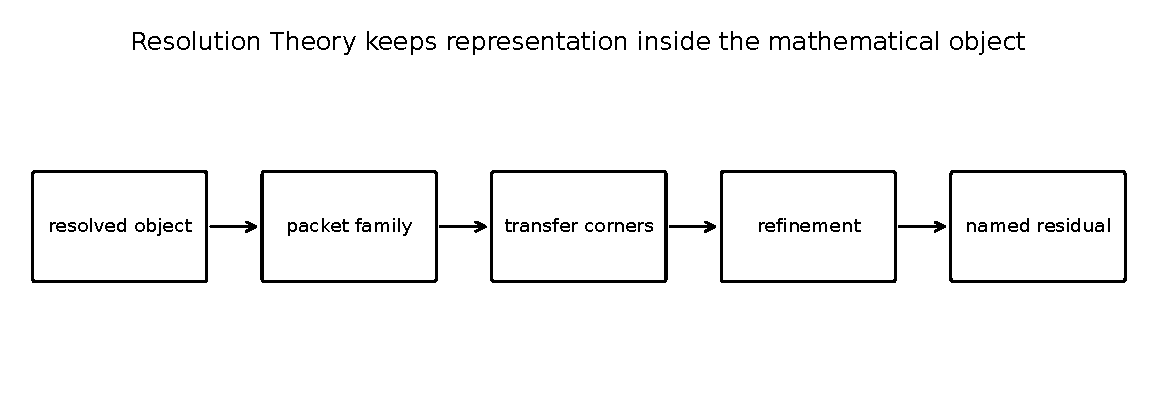
\includegraphics[width=.97\textwidth]{01_architecture.pdf}
\caption{The basic resolved object. A representation is retained as mathematical structure rather than discarded after use.}
\label{fig:architecture}
\end{figure}

\subsection{Main results}

The article proves twelve groups of results.

\begin{enumerate}
\item Finite resolved Hilbert systems admit exact block reconstruction, packet Parseval identities, coherent refinement, selective compression, budget tolerance duality, and common refinement criteria.
\item The space of finite resolutions carries a permutation invariant metric. Mixed block fields and transfer energy distributions vary Lipschitz continuously with the source and target resolutions.
\item Smooth projector families admit canonical unitary transport. A covariant derivative separates physical evolution from chart motion. A spectral gap of the commutant Laplacian converts small commutator leakage into a nearby exact reducing projector.
\item Resolved linking systems satisfy a universal corner extension law and admit faithful projector corner representations. Recognition recovers the abstract system and representation commutes with refinement.
\item Weighted block Schur classes form Banach star algebras. Small weighted perturbations are inverse closed by a Neumann theorem, and block diagonal dominance produces inverse packet path expansions with quantitative off diagonal decay.
\item Countable systems reconstruct bounded transfers strongly, compact and Schatten transfers in their natural norms, and linking algebra elements in finite windows. Strict multiplier limits, packet Karoubi objects, normal states, quadratic forms, and measurable fields complete the declared infinite sectors.
\item Self adjoint unbounded generators are controlled through reducing packets, graph norms, forms, resolvents, bounded transforms, strong resolvent convergence, and commutator leakage bounds.
\item Smooth nonlinear maps admit exact packet jets, operadic composition, weighted analytic inversion, Newton certificates, countable multilinear reconstruction, semilinear Duhamel trees, Hamiltonian structure, and stochastic second order corrections.
\item Finite and countable atomic Resolution Logic organize Boolean predicates and complete lattice certificates over refinement maps, with sound linear and multilinear error transport.
\item Fourier, wavelet, polyphase, quantum, and arithmetic packet systems are concrete realizations. The arithmetic realization separates the deterministic sieve direction from survivor residuals and identifies the residual character band by a finite Gauss transform.
\item Finite Galois theory embeds through subgroup averaging projectors. Normality becomes central compatibility, trace and norm become packet transfers, nonnormal extensions become conjugate atlases, and Mackey double cosets become transition packets.
\item Ramification groups give a nested resolution whose weighted unresolved ranks equal the Artin conductor. Haar averaging extends the construction to profinite groups, while Hilbert 90, Brauer classes, etale Galois categories, and Tannakian fiber functors describe effective descent and its exact obstructions.
\end{enumerate}

\subsection{Status and scope}

Several representation statements are resolved consequences of classical operator algebra once the packet hierarchy has been declared. They are included because preservation of the named hierarchy is the central question. The metric stability, commutant gap, weighted packet inverse, covariant transport, countable atomic logic, arithmetic sieve decomposition, and projector formulation of the semisimple Galois correspondence are proved directly in the resolved language.

No claim is made that every operator family has a useful packetization, that refinement always lowers computational cost, that a local Neumann theorem gives global spectral invariance for every weighted algebra, or that every resolved monoidal category has a Hilbert space fiber functor. These boundaries are stated in \cref{sec:boundaries}.

\section{Finite resolved transfer systems}\label{sec:finite}

\subsection{Axioms and concrete realization}

\begin{definition}[Finite resolved transfer system]\label{def:finite_resolved_system}
A finite resolved transfer system consists of the following data.
\begin{enumerate}[label=\textup{(R\arabic*)}]
\item Every object \(X\) has a finite packet set \(I_X\) and packet spaces \(X_i\).
\item Every transfer space has a finite decomposition
\[
 \Tcal(X,Y)
 \cong
 \bigoplus_{a\in I_Y,\,i\in I_X}
 \Tcal_{ai}(X,Y).
\]
\item Reconstruction is faithful. A transfer is determined by its packet blocks.
\item Composition is matrix composition
\[
 (S\circ T)_{ci}
 =
 \sum_{a\in I_Y}S_{ca}T_{ai}.
\]
\item Identity transfers are diagonal.
\item A dagger interchanges source and target blocks.
\item Tensor products distribute over packets.
\item A refinement replaces a packet by finitely many orthogonal descendants, and coarse transfers are sums of descendant transfers.
\item Transfer spaces are normed and composition is continuous.
\end{enumerate}
\end{definition}

\begin{theorem}[Mixed block representation]\label{thm:mixed_blocks}
Let
\[
 \Hh=\bigoplus_{i\in I}\Hh_i,
 \qquad
 \K=\bigoplus_{a\in A}\K_a
\]
with orthogonal projectors \(P_i\) and \(Q_a\). The map
\[
 \Phi_{\Qcal\leftarrow\Pcal}:
 \B(\Hh,\K)
 \longrightarrow
 \bigoplus_{a,i}\B(\Hh_i,\K_a),
 \qquad
 T\longmapsto(Q_aTP_i)_{a,i}
\]
is a linear bijection. Its inverse is
\[
 \Rcal((T_{ai}))=\sum_{a,i}T_{ai}.
\]
For a third resolved space \(\Lcal=\bigoplus_c\Lcal_c\),
\[
 \Phi_{\mathcal S\leftarrow\Pcal}(ST)_{ci}
 =
 \sum_a
 \Phi_{\mathcal S\leftarrow\Qcal}(S)_{ca}
 \Phi_{\Qcal\leftarrow\Pcal}(T)_{ai}.
\]
Moreover,
\[
 \Phi(T^*)_{ia}
 =
 \Phi(T)_{ai}^*.
\]
\end{theorem}

\begin{proof}
Insert the two resolutions of the identity:
\[
 T
 =
 I_{\K}TI_{\Hh}
 =
 \left(\sum_aQ_a\right)
 T
 \left(\sum_iP_i\right)
 =
 \sum_{a,i}Q_aTP_i.
\]
This proves reconstruction and faithfulness. Conversely, a finite family of maps from \(\Hh_i\) to \(\K_a\) defines one map on the direct sums by the same sum.

For composition, insert the intermediate identity:
\[
 R_cSTP_i
 =
 R_cS\left(\sum_aQ_a\right)TP_i
 =
 \sum_a(R_cSQ_a)(Q_aTP_i).
\]
The adjoint identity follows from
\[
 (Q_aTP_i)^*=P_iT^*Q_a.
\]
\end{proof}

\begin{corollary}[Linking algebra realization]\label{cor:linking_algebra}
For one resolved Hilbert space \(\Hh=\bigoplus_i\Hh_i\), the corner algebra
\[
 \bigoplus_{i,j}\B(\Hh_j,\Hh_i)
\]
with matrix composition and blockwise adjoint is canonically star isomorphic to \(\B(\Hh)\).
\end{corollary}

\begin{proof}
Apply \cref{thm:mixed_blocks} with equal source and target resolutions. The composition and adjoint formulas identify the algebraic operations.
\end{proof}

\begin{figure}[t]
\centering
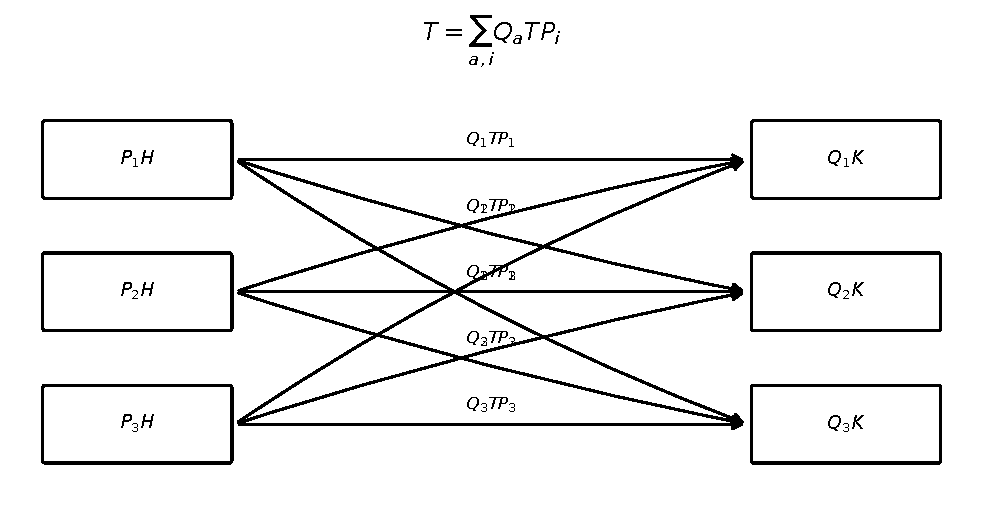
\includegraphics[width=.90\textwidth]{02_block_reconstruction.pdf}
\caption{The transfer field of an operator. Reconstruction is the sum of all mixed corners.}
\label{fig:block_reconstruction}
\end{figure}

\subsection{Orthogonal accounting}

\begin{theorem}[Packet Parseval identity]\label{thm:packet_parseval}
If \(T:\Hh\to\K\) is Hilbert Schmidt, then
\[
 \boxed{
 \norm{T}_{\mathrm{HS}}^2
 =
 \sum_{a,i}\norm{Q_aTP_i}_{\mathrm{HS}}^2.
 }
\]
Distinct packet blocks are orthogonal in the Hilbert Schmidt inner product.
\end{theorem}

\begin{proof}
For two blocks,
\[
 \langle Q_aTP_i,Q_bTP_j\rangle_{\mathrm{HS}}
 =
 \Tr(P_iT^*Q_aQ_bTP_j).
\]
If \(a\ne b\), then \(Q_aQ_b=0\). If \(i\ne j\), cyclicity of the trace brings \(P_jP_i=0\) together. The reconstruction from \cref{thm:mixed_blocks} is therefore an orthogonal sum.
\end{proof}

\begin{definition}[Transfer energy distribution]\label{def:transfer_energy}
For nonzero Hilbert Schmidt \(T\), define
\[
 p_{ai}(T)
 =
 \frac{\norm{Q_aTP_i}_{\mathrm{HS}}^2}
 {\norm{T}_{\mathrm{HS}}^2}.
\]
The transfer entropy is
\[
 H_{\Qcal\leftarrow\Pcal}(T)
 =
 -\sum_{a,i}p_{ai}(T)\log p_{ai}(T),
\]
with the convention \(0\log0=0\).
\end{definition}

\begin{proposition}[Unitary invariance and tensor additivity]\label{prop:entropy_properties}
Packetwise unitaries preserve the transfer energy distribution. If \(S\) and \(T\) are nonzero Hilbert Schmidt maps equipped with product packet resolutions, then
\[
 H(S\otimes T)=H(S)+H(T).
\]
\end{proposition}

\begin{proof}
Packetwise unitaries preserve each Hilbert Schmidt block norm. For tensor products,
\[
 p_{(b,a),(j,i)}(S\otimes T)
 =
 p_{bj}(S)p_{ai}(T).
\]
The entropy of a product probability distribution is the sum of the entropies.
\end{proof}

\subsection{Refinement and coarsening}

Suppose
\[
 P_i=\sum_{\alpha\in C(i)}P_{i\alpha},
 \qquad
 Q_a=\sum_{\beta\in D(a)}Q_{a\beta}
\]
are finite orthogonal refinements.

\begin{theorem}[Exact refinement law]\label{thm:exact_refinement}
For every bounded operator \(T\),
\[
 \boxed{
 Q_aTP_i
 =
 \sum_{\beta\in D(a)}
 \sum_{\alpha\in C(i)}
 Q_{a\beta}TP_{i\alpha}.
 }
\]
If \(S\) and \(T\) are composable, coarsening the fine block product gives the coarse block product.
\end{theorem}

\begin{proof}
Insert the two refinement identities on the left and right of \(T\). For composition, expand both maps at the fine level, multiply, and sum over descendant intermediate packets. The descendant projectors sum to the coarse intermediate projector.
\end{proof}

\begin{theorem}[Resolution double category]\label{thm:double_category}
Finite resolved Hilbert spaces form a thin strict double category with resolved Hilbert spaces as objects, bounded maps as horizontal arrows, refinement maps on one underlying space as vertical arrows, and the block coarsening identity as the unique compatible square.
\end{theorem}

\begin{proof}
Horizontal composition is operator composition. Vertical composition is ancestry of packets. A square states that a coarse block is the sum of its descendants. The interchange law is finite distributivity and is equivalent to \cref{thm:exact_refinement}. This is a strict resolved instance of the double categorical framework \Rcite{R13}.
\end{proof}

\begin{figure}[t]
\centering
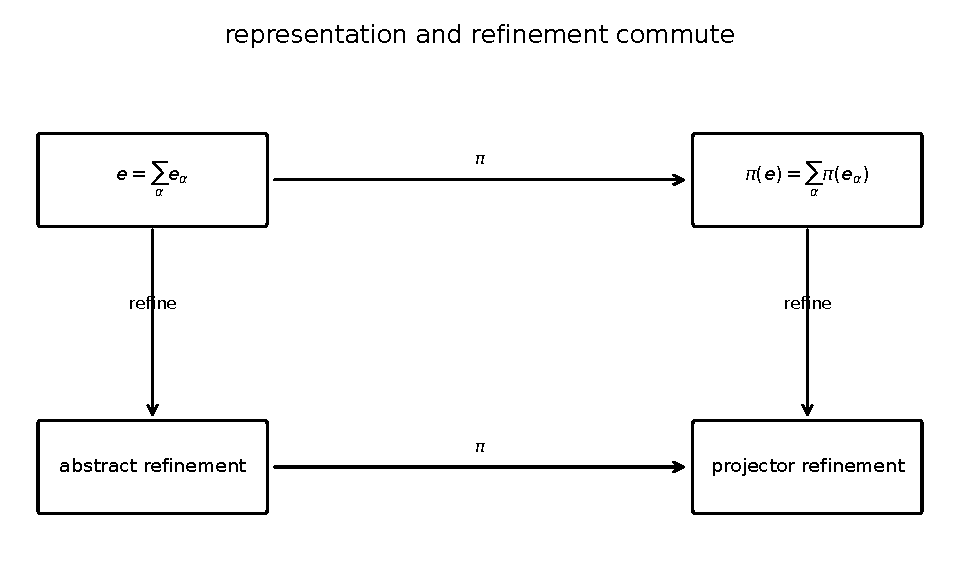
\includegraphics[width=.84\textwidth]{05_refinement_naturality.pdf}
\caption{Refinement is a second mathematical direction. It is not another physical evolution.}
\label{fig:refinement_naturality_preview}
\end{figure}

\subsection{Compression and named residuals}

Let \(E\subseteq A\times I\) be a selected set of packet edges. Define
\[
 C_E(T)=\sum_{(a,i)\in E}Q_aTP_i,
 \qquad
 R_E(T)=T-C_E(T).
\]

\begin{theorem}[Selective compression]\label{thm:selective_compression}
On the Hilbert space of Hilbert Schmidt operators, \(C_E\) is the orthogonal projection onto the span of the selected block subspaces. Moreover,
\[
 \boxed{
 \norm{T-C_E(T)}_{\mathrm{HS}}^2
 =
 \sum_{(a,i)\notin E}
 \norm{Q_aTP_i}_{\mathrm{HS}}^2.
 }
\]
Among all Hilbert Schmidt operators supported on \(E\), \(C_E(T)\) is the unique best approximation to \(T\).
\end{theorem}

\begin{proof}
The block subspaces are orthogonal by \cref{thm:packet_parseval}. Projection onto their selected direct sum keeps exactly those blocks. The Pythagorean identity gives the residual norm and uniqueness.
\end{proof}

\begin{corollary}[Best diagonal approximation]\label{cor:best_diagonal}
For one resolution \(\{P_i\}\), the map
\[
 \Ecal(T)=\sum_iP_iTP_i
\]
is the Hilbert Schmidt orthogonal projection onto the block diagonal algebra.
\end{corollary}

\begin{proof}
Use \cref{thm:selective_compression} with \(E=\{(i,i)\}\).
\end{proof}

\begin{figure}[t]
\centering
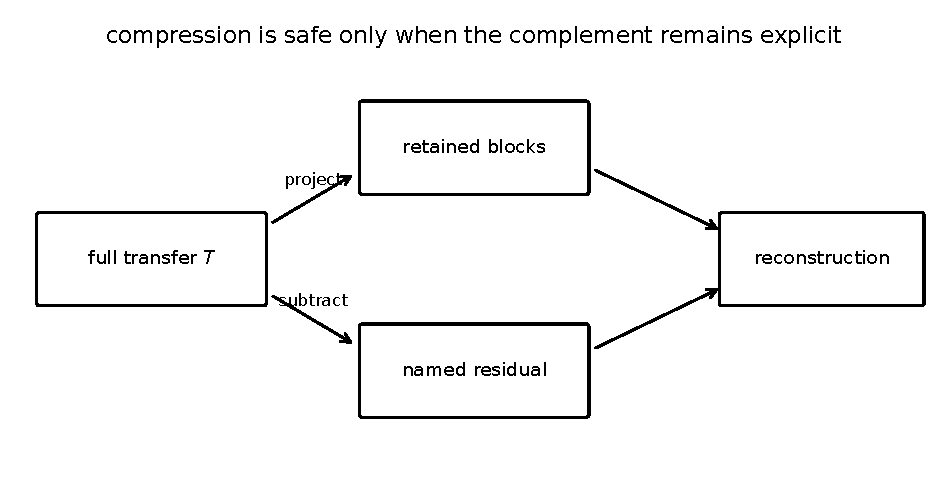
\includegraphics[width=.82\textwidth]{13_compression_residual.pdf}
\caption{Compression is a projection with an explicit complementary residual.}
\label{fig:compression_residual}
\end{figure}

\subsection{Compatibility of resolutions}

\begin{theorem}[Common refinement criterion]\label{thm:common_refinement}
Two finite orthogonal resolutions \(\{P_i\}\) and \(\{Q_a\}\) on one Hilbert space admit a common orthogonal refinement if and only if
\[
 [P_i,Q_a]=0
 \qquad
 \text{for every }i,a.
\]
When they commute, the nonzero products \(P_iQ_a\) form a common refinement.
\end{theorem}

\begin{proof}
If the projectors commute, every product \(P_iQ_a\) is a self adjoint idempotent. Distinct products are orthogonal, their sum is the identity, and the two original families are recovered by summation.

Conversely, if \(\{R_\gamma\}\) refines both families, every \(P_i\) and \(Q_a\) is a sum of members of the same orthogonal family. Such sums commute.
\end{proof}

\begin{remark}[Projector atlases]\label{rem:projector_atlas}
If the resolutions do not commute, the products \(P_iQ_a\) need not be projectors. The correct replacement is an atlas of valid charts connected by mixed corners \(Q_aTP_i\). The representation theorem does not erase this incompatibility.
\end{remark}

\begin{figure}[t]
\centering
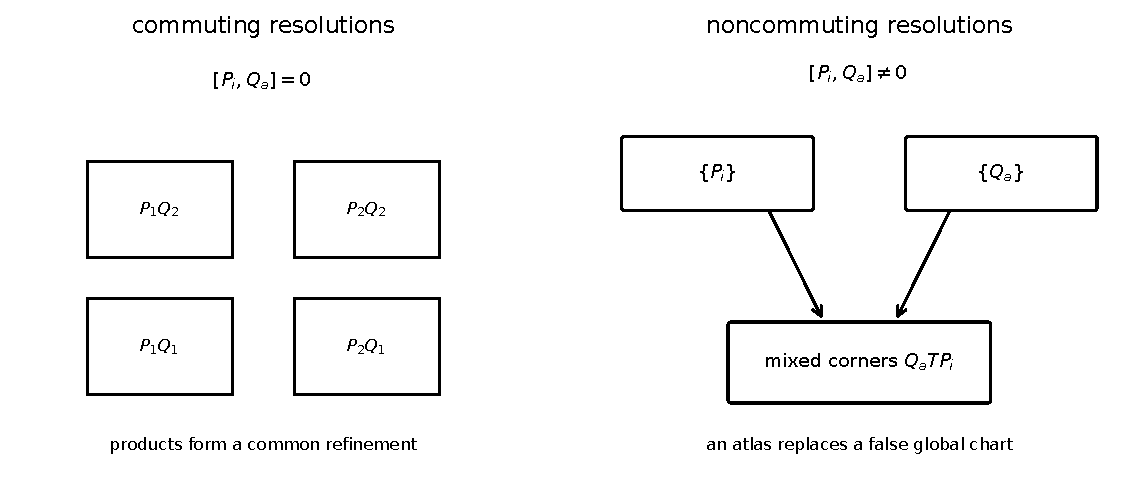
\includegraphics[width=.92\textwidth]{03_common_refinement_atlas.pdf}
\caption{Commuting resolutions merge into one chart. Noncommuting resolutions remain an atlas.}
\label{fig:common_refinement_atlas}
\end{figure}

\begin{theorem}[Common reducing projector criterion]\label{thm:commutant_projector}
Let \(\Fcal=\{A_1,\ldots,A_r\}\) be a finite operator family. It admits a nontrivial exact two packet reducing resolution if and only if its commutant
\[
 \Fcal'
 =
 \{X:[X,A_k]=0\text{ for all }k\}
\]
contains a projection other than \(0\) and \(I\).
\end{theorem}

\begin{proof}
A reducing projector commutes with every member of the family. Conversely, a nontrivial projection in the commutant yields the resolution \(\{P,I-P\}\), and every operator is block diagonal in it.
\end{proof}

For self adjoint \(A_k\), define the commutant Laplacian
\[
 \Lcal_{\Fcal}(X)
 =
 \sum_k[A_k,[A_k,X]].
\]

\begin{theorem}[Commutant Laplacian identity]\label{thm:commutant_laplacian}
On Hilbert Schmidt space,
\[
 \boxed{
 \langle X,\Lcal_{\Fcal}(X)\rangle_{\mathrm{HS}}
 =
 \sum_k\norm{[A_k,X]}_{\mathrm{HS}}^2.
 }
\]
Consequently, \(\Lcal_{\Fcal}\) is positive semidefinite and
\[
 \ker\Lcal_{\Fcal}=\Fcal'.
\]
\end{theorem}

\begin{proof}
For one self adjoint \(A\), direct expansion and cyclicity of trace give
\[
 \langle X,[A,[A,X]]\rangle_{\mathrm{HS}}
 =
 \norm{[A,X]}_{\mathrm{HS}}^2.
\]
Sum over the family. The quadratic form vanishes exactly when all commutators vanish.
\end{proof}

\begin{theorem}[Finite lattice of coordinate resolutions]\label{thm:partition_lattice}
If every resolution coarsens one fixed finite atomic commuting resolution, then the resolution poset is the partition lattice of the atom set. The meet consists of all nonempty block intersections. The join is the equivalence relation generated by the two block relations.
\end{theorem}

\begin{proof}
The intersection partition is the greatest common refinement. The transitive closure of the two block relations is the least common coarsening.
\end{proof}

\begin{theorem}[Finite unitary gluing]\label{thm:unitary_gluing}
Let \(\{U_a\}\) cover a parameter space. Suppose each \(U_a\) carries a local packet model and unitary transition maps \(g_{ab}\) satisfy
\[
 g_{aa}=I,
 \qquad
 g_{ab}=g_{ba}^{-1},
 \qquad
 g_{ab}g_{bc}=g_{ac}
\]
on triple overlaps. Then the local models glue to a Hermitian vector bundle. Compatible local sections glue uniquely.
\end{theorem}

\begin{proof}
Take the disjoint union of the local trivial bundles and impose the transition equivalence relation. The cocycle law gives transitivity. Unitarity preserves the Hermitian structure. Compatible sections define one global equivalence class at every point.
\end{proof}

\section{Geometry and stability of resolution space}\label{sec:geometry}

The finite packet calculus is algebraic, but a resolution may move under perturbation, learning, parameter change, or physical transport. The representation itself therefore has a geometry. This section supplies a metric, a stability theorem for transfer blocks, a covariant transport law, and a gap criterion for approximate reducing packets.

\subsection{Metrics and stable transfer fields}

For orthogonal projections on one finite dimensional Hilbert space, define
\[
 d_{\mathrm{ch}}(P,Q)
 =
 \frac1{\sqrt2}\norm{P-Q}_{\mathrm{HS}}.
\]

\begin{proposition}[Chordal projector metric]\label{prop:chordal_metric}
The function \(d_{\mathrm{ch}}\) is a metric on the set of orthogonal projections on a fixed finite dimensional Hilbert space.
\end{proposition}

\begin{proof}
Nonnegativity, symmetry, and separation follow from the Hilbert Schmidt norm. The triangle inequality is inherited from that norm. The normalization is conventional and agrees with the Euclidean norm of the sines of the principal angles when the ranks agree.
\end{proof}

A finite resolution is unordered. For two resolutions with the same packet count, define
\[
 d_{\mathrm{res}}(\Pcal,\widetilde\Pcal)^2
 =
 \min_{\sigma}
 \sum_i
 d_{\mathrm{ch}}(P_i,\widetilde P_{\sigma(i)})^2,
\]
where the minimum is over packet permutations.

\begin{theorem}[Permutation invariant resolution metric]\label{thm:resolution_metric}
Modulo relabeling, \(d_{\mathrm{res}}\) is a metric on finite resolutions with a fixed packet count.
\end{theorem}

\begin{proof}
Only the triangle inequality needs comment. Choose optimal matchings from \(\Pcal\) to \(\Qcal\) and from \(\Qcal\) to \(\Rcal\). Their composition is an admissible matching from \(\Pcal\) to \(\Rcal\). Minkowski's inequality for the vector of chordal distances gives the triangle inequality. The direct optimum can only be smaller.
\end{proof}

\begin{figure}[t]
\centering
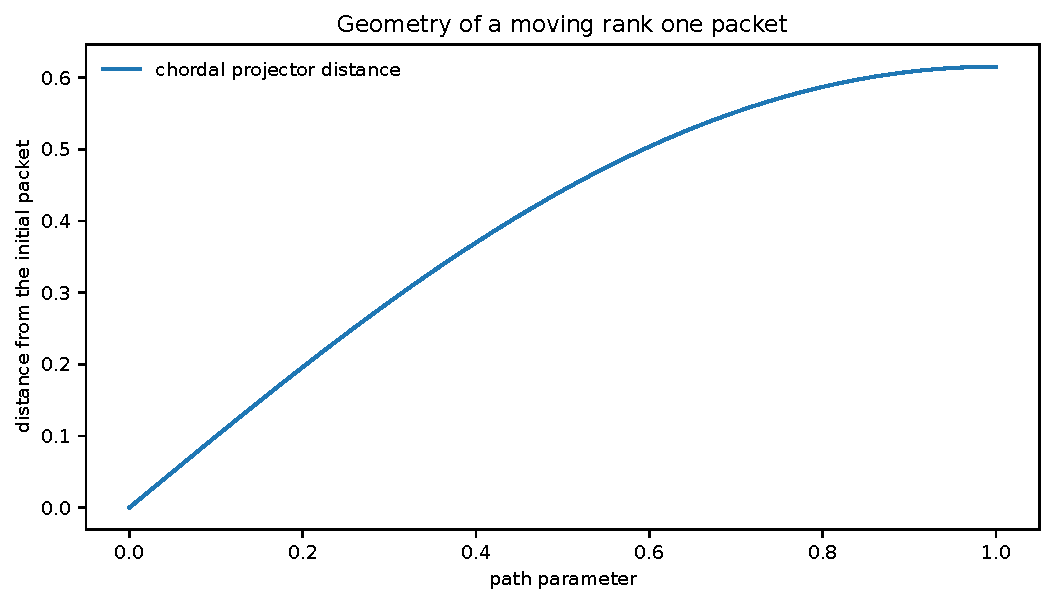
\includegraphics[width=.76\textwidth]{14_resolution_metric.pdf}
\caption{A moving packet is a path in resolution space. The geometry records representational motion independently of the operator being represented.}
\label{fig:resolution_metric}
\end{figure}

For ordered packet families, write
\[
 d_{\mathrm{ord}}(\Pcal,\widetilde\Pcal)^2
 =
 \frac12\sum_i\norm{P_i-\widetilde P_i}_{\mathrm{HS}}^2.
\]

\begin{theorem}[Lipschitz stability of mixed block fields]\label{thm:block_field_stability}
Let \(T:\Hh\to\K\) be Hilbert Schmidt. Let \(\Pcal,\widetilde\Pcal\) resolve the source and let \(\Qcal,\widetilde\Qcal\) resolve the target, with corresponding packet labels. Put
\[
 \Delta_T^2
 =
 \sum_{a,i}
 \norm{Q_aTP_i-\widetilde Q_aT\widetilde P_i}_{\mathrm{HS}}^2.
\]
Then
\[
 \boxed{
 \Delta_T
 \leq
 2\norm{T}_{\mathrm{HS}}
 \left(
 d_{\mathrm{ord}}(\Pcal,\widetilde\Pcal)^2
 +
 d_{\mathrm{ord}}(\Qcal,\widetilde\Qcal)^2
 \right)^{1/2}.
 }
\]
The same conclusion holds for unordered families after choosing optimal packet matchings.
\end{theorem}

\begin{proof}
Split each block difference as
\[
 (Q_a-\widetilde Q_a)TP_i
 +
 \widetilde Q_aT(P_i-\widetilde P_i).
\]
Using \(\norm{x+y}^2\leq2\norm{x}^2+2\norm{y}^2\), packet Parseval on the unaffected side, and \(\norm{AXB}_{\mathrm{HS}}\leq\norm A\norm{B}\norm X_{\mathrm{HS}}\), we obtain
\[
 \Delta_T^2
 \leq
 2\norm T_{\mathrm{HS}}^2
 \left(
 \sum_a\norm{Q_a-\widetilde Q_a}_{\mathrm{HS}}^2
 +
 \sum_i\norm{P_i-\widetilde P_i}_{\mathrm{HS}}^2
 \right).
\]
The definition of \(d_{\mathrm{ord}}\) gives the claim.
\end{proof}

\begin{corollary}[Stability of transfer energy distributions]\label{cor:energy_distribution_stability}
Assume \(T\ne0\). Let \(p_{ai}\) and \(\widetilde p_{ai}\) be the transfer energy distributions of \(T\) in the two pairs of resolutions. Then
\[
 \boxed{
 \TV(p,\widetilde p)
 \leq
 \frac{\Delta_T}{\norm T_{\mathrm{HS}}}
 \leq
 2
 \left(
 d_{\mathrm{ord}}(\Pcal,\widetilde\Pcal)^2
 +
 d_{\mathrm{ord}}(\Qcal,\widetilde\Qcal)^2
 \right)^{1/2}.
 }
\]
\end{corollary}

\begin{proof}
For block vectors \(u_{ai}=Q_aTP_i\) and \(v_{ai}=\widetilde Q_aT\widetilde P_i\),
\[
 \sum_{a,i}
 \left|
 \norm{u_{ai}}^2-\norm{v_{ai}}^2
 \right|
 \leq
 \left(\sum_{a,i}\norm{u_{ai}-v_{ai}}^2\right)^{1/2}
 \left(\sum_{a,i}(\norm{u_{ai}}+\norm{v_{ai}})^2\right)^{1/2}.
\]
Packet Parseval makes the second factor at most \(2\norm T_{\mathrm{HS}}\). Divide by \(2\norm T_{\mathrm{HS}}^2\).
\end{proof}

\begin{figure}[t]
\centering
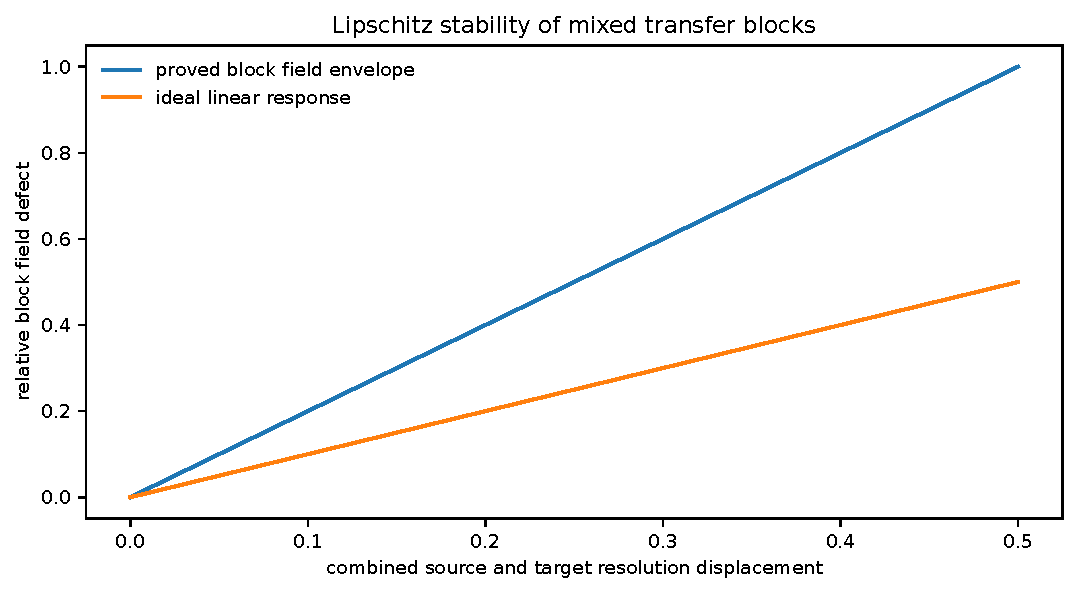
\includegraphics[width=.77\textwidth]{15_block_stability.pdf}
\caption{Resolution displacement controls the defect of the full mixed block field and therefore controls its energy distribution.}
\label{fig:block_stability}
\end{figure}

\subsection{Covariant motion of packet families}

Let \((P_i(t))_{i=1}^m\) be a continuously differentiable complete orthogonal projector family. Define
\[
 K_{\Pcal}(t)
 =
 \sum_i\dot P_i(t)P_i(t).
\]

\begin{theorem}[Canonical unitary transport of a moving resolution]\label{thm:kato_transport}
The generator \(K_{\Pcal}(t)\) is skew adjoint. If
\[
 \dot U_{\Pcal}(t)
 =
 K_{\Pcal}(t)U_{\Pcal}(t),
 \qquad
 U_{\Pcal}(0)=I,
\]
then \(U_{\Pcal}(t)\) is unitary and
\[
 \boxed{
 P_i(t)
 =
 U_{\Pcal}(t)P_i(0)U_{\Pcal}(t)^*
 }
\]
for every packet. This is the canonical parallel transport of the resolution path.
\end{theorem}

\begin{proof}
Differentiating \(P_i^2=P_i\) and summing gives
\[
 K_{\Pcal}+K_{\Pcal}^*
 =
 \sum_i(\dot P_iP_i+P_i\dot P_i)
 =
 \sum_i\dot P_i
 =0.
\]
Hence the propagator is unitary. Orthogonality and completeness imply
\[
 [K_{\Pcal},P_i]=\dot P_i.
\]
Differentiate \(U_{\Pcal}^*P_iU_{\Pcal}\). The derivative is zero, so the quantity equals \(P_i(0)\).
\end{proof}

\begin{proposition}[Covariant derivative of a moving transfer]\label{prop:covariant_transfer_derivative}
Let source and target resolutions move with generators \(K_{\Pcal}\) and \(K_{\Qcal}\). For a differentiable transfer \(T(t)\), define
\[
 \boxed{
 \nabla T
 =
 \dot T-K_{\Qcal}T+TK_{\Pcal}.
 }
\]
If
\[
 \widehat T(t)
 =
 U_{\Qcal}(t)^*T(t)U_{\Pcal}(t),
\]
then
\[
 \boxed{
 \frac d{dt}\widehat T
 =
 U_{\Qcal}^*(\nabla T)U_{\Pcal}.
 }
\]
Thus \(\nabla T\) measures physical transfer variation after chart motion has been removed.
\end{proposition}

\begin{proof}
Differentiate the transported transfer and use \(\dot U=KU\) and \((U^*)'=-U^*K\).
\end{proof}

\begin{figure}[t]
\centering
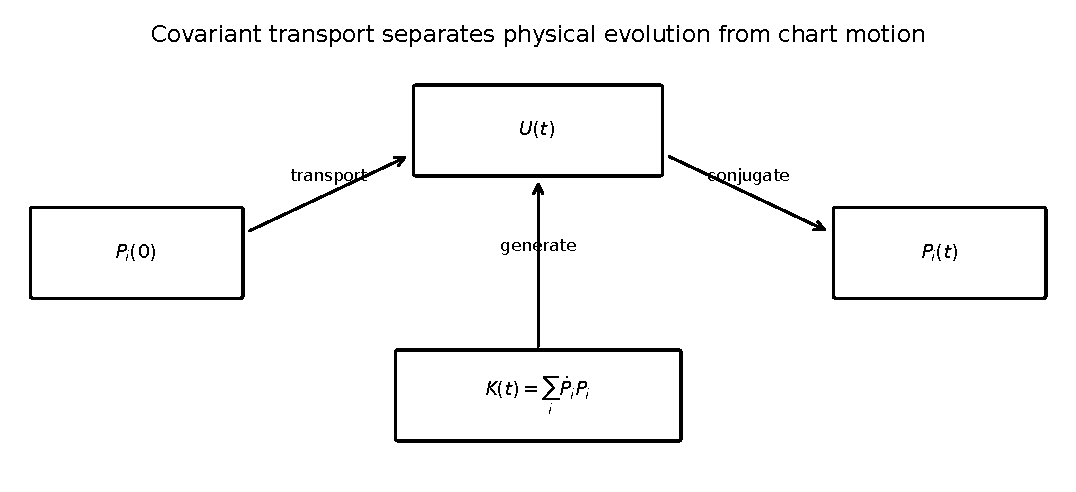
\includegraphics[width=.88\textwidth]{16_kato_transport.pdf}
\caption{Canonical unitary transport freezes a moving packet family and leaves a covariant derivative for the physical transfer.}
\label{fig:kato_transport}
\end{figure}

\subsection{Commutant gaps and exact nearby packets}

Let \(A_1,\ldots,A_r\) be self adjoint matrices. On the Hilbert Schmidt operator space, define
\[
 \Lcal_{\Acal}(X)
 =
 \sum_{k=1}^r[A_k,[A_k,X]].
\]
Let \(\Ecal_{\Acal}\) be the Hilbert Schmidt orthogonal projection onto the common commutant. When its orthogonal complement is nonzero, let \(\gamma_{\Acal}\) be the smallest positive eigenvalue of \(\Lcal_{\Acal}\) there. If the complement is zero, every matrix already lies in the commutant and the estimates below are vacuous.

\begin{theorem}[Commutant gap stability]\label{thm:commutant_gap_stability}
For every matrix \(X\),
\[
 \boxed{
 \norm{X-\Ecal_{\Acal}X}_{\mathrm{HS}}^2
 \leq
 \frac1{\gamma_{\Acal}}
 \sum_{k=1}^r\norm{[A_k,X]}_{\mathrm{HS}}^2.
 }
\]
Let \(P\) be an orthogonal projection and put
\[
 \varepsilon(P)
 =
 \sum_k\norm{[A_k,P]}_{\mathrm{HS}}^2.
\]
If
\[
 \varepsilon(P)<\frac{\gamma_{\Acal}}4,
\]
then there is an orthogonal projection \(Q\) in the exact common commutant with
\[
 \boxed{
 \norm{P-Q}
 \leq
 2\sqrt{\frac{\varepsilon(P)}{\gamma_{\Acal}}}.
 }
\]
The rank of \(Q\) equals the rank of \(P\).
\end{theorem}

\begin{proof}
The commutant Laplacian identity gives
\[
 \langle X,\Lcal_{\Acal}X\rangle_{\mathrm{HS}}
 =
 \sum_k\norm{[A_k,X]}_{\mathrm{HS}}^2.
\]
The spectral gap on the orthogonal complement of the kernel gives the first estimate. Put \(Y=\Ecal_{\Acal}P\). Then \(Y\) is self adjoint, belongs to the commutant, and
\[
 \norm{P-Y}
 \leq
 \norm{P-Y}_{\mathrm{HS}}
 <\frac12.
\]
Let \(Q\) be the spectral projection of \(Y\) for \([1/2,\infty)\). Functional calculus keeps \(Q\) in the commutant. The standard spectral projection perturbation estimate gives
\[
 \norm{P-Q}\leq2\norm{P-Y}.
\]
The same gap estimate preserves the rank. The perturbation step is a standard consequence of spectral projection stability \Rcite{R10}.
\end{proof}

\begin{figure}[t]
\centering
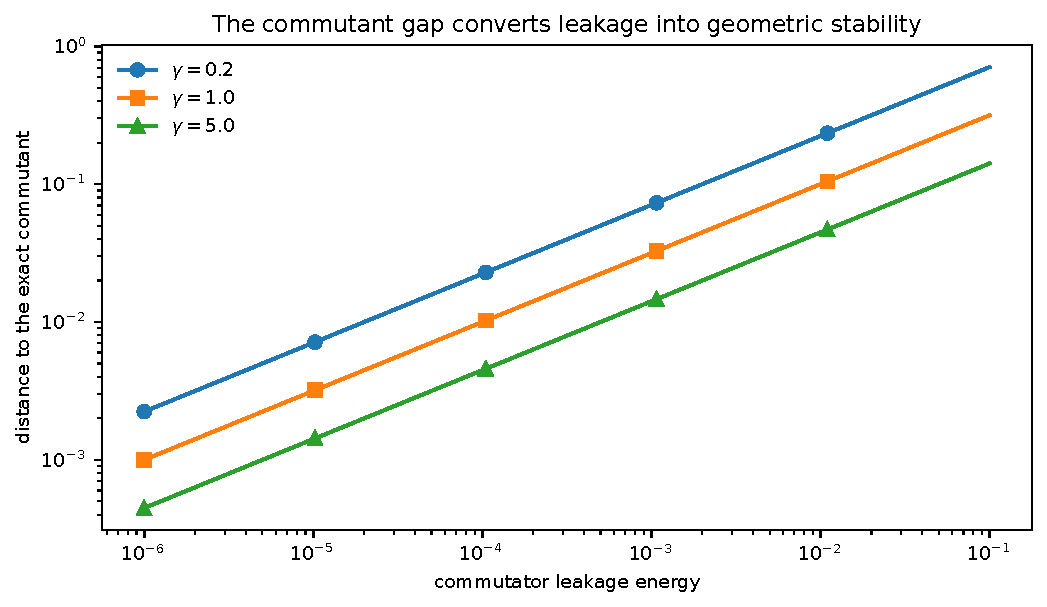
\includegraphics[width=.76\textwidth]{17_commutant_gap.pdf}
\caption{A positive commutant gap turns approximate invariance into quantitative proximity to an exact reducing packet.}
\label{fig:commutant_gap}
\end{figure}

\subsection{Approximate descent and compression profiles}

\begin{proposition}[Path accumulation under approximate gluing]\label{prop:path_accumulation}
Let unitary chart transitions have elementary cocycle defect at most \(\delta\) in operator norm. If two homotopic paths between the same charts differ by at most \(N\) elementary triangle moves, then their transported vectors differ by at most
\[
 \boxed{N\delta\norm v.}
\]
\end{proposition}

\begin{proof}
One triangle move replaces one two edge transport by the direct transition and changes a vector by at most \(\delta\norm v\). All remaining transitions are unitary. A telescoping estimate over the moves gives the result.
\end{proof}

Let the block energies of a Hilbert Schmidt transfer be ordered as
\[
 e_1\geq e_2\geq\cdots\geq e_M\geq0.
\]
Define
\[
 E(k)=\left(\sum_{j>k}e_j\right)^{1/2},
 \qquad
 C(\varepsilon)=\min\{k:E(k)\leq\varepsilon\}.
\]

\begin{theorem}[Budget tolerance duality]\label{thm:budget_tolerance}
For every \(k\) and \(\varepsilon\geq0\),
\[
 \boxed{
 C(\varepsilon)\leq k
 \quad\Longleftrightarrow\quad
 E(k)\leq\varepsilon.
 }
\]
Thus the optimal residual curve and the minimum complexity curve are monotone generalized inverses.
\end{theorem}

\begin{proof}
If \(C(\varepsilon)\leq k\), some budget no larger than \(k\) achieves residual at most \(\varepsilon\). Optimality and monotonicity of \(E\) give \(E(k)\leq\varepsilon\). The converse is immediate from the defining minimum.
\end{proof}

\section{Universal representation of resolved \texorpdfstring{\(C^*\)}{C star} systems}\label{sec:universal}

The finite Hilbert space calculus suggests an abstract object in which the packet hierarchy is declared before any concrete Hilbert space is chosen. The relevant ambient structure is a linking algebra. Classical \(C^*\) category theory supplies the surrounding representation framework \Rcite{R2}, \Rcite{R3}, \Rcite{R4}.

\begin{definition}[Resolved linking system]\label{def:resolved_linking_system}
A resolved linking system is a tuple
\[
 \Acal
 =
 \left(
 A,
 \{p_x\}_{x\in X},
 \{e_{x,i}\}_{i\in I_x},
 \mathfrak F
 \right)
\]
with the following properties.
\begin{enumerate}[label=\textup{(L\arabic*)}]
\item \(A\) is a unital complex \(C^*\) algebra.
\item The object projections are mutually orthogonal and complete:
\[
 p_xp_y=\delta_{xy}p_x,
 \qquad
 \sum_{x\in X}p_x=1_A.
\]
\item For each object \(x\), the packet projections are mutually orthogonal and resolve \(p_x\):
\[
 e_{x,i}e_{x,j}=\delta_{ij}e_{x,i},
 \qquad
 \sum_{i\in I_x}e_{x,i}=p_x.
\]
\item Every declared refinement in \(\mathfrak F\) replaces one packet by a finite orthogonal family.
\end{enumerate}
The object transfer space is \(p_yAp_x\), and the packet transfer space is \(e_{y,a}Ae_{x,i}\).
\end{definition}

\begin{proposition}[Corner category]\label{prop:corner_category}
A resolved linking system determines a finite \(C^*\) category whose objects are the projections \(p_x\) and whose morphism spaces are \(p_yAp_x\). Composition is multiplication in \(A\), and the dagger is the \(C^*\) adjoint.
\end{proposition}

\begin{proof}
If \(a\in p_yAp_x\) and \(b\in p_zAp_y\), then
\[
 ba=p_zbp_y\,p_yap_x=p_z(ba)p_x\in p_zAp_x.
\]
Associativity, identities, the norm, and the \(C^*\) identity are inherited from \(A\). The adjoint reverses source and target.
\end{proof}

\begin{theorem}[Universal extension of compatible corner maps]\label{thm:universal_corner_extension}
Let \(\Acal\) be a resolved linking system with finite object set. Let \(K\) be a Hilbert space with mutually orthogonal projections \(Q_x\) satisfying
\[
 \sum_xQ_x=I_K.
\]
Suppose that for every pair \(x,y\) there is a linear map
\[
 F_{yx}:p_yAp_x\longrightarrow Q_y\B(K)Q_x
\]
such that
\[
 F_{zy}(b)F_{yx}(a)=F_{zx}(ba),
\]
\[
 F_{xy}(a^*)=F_{yx}(a)^*,
\]
and
\[
 F_{xx}(p_x)=Q_x.
\]
Then there is a unique unital star homomorphism
\[
 \widetilde F:A\longrightarrow\B(K)
\]
whose restriction to every corner is \(F_{yx}\).
\end{theorem}

\begin{proof}
Every \(a\in A\) has the finite corner expansion
\[
 a=\sum_{x,y}p_yap_x.
\]
Define
\[
 \widetilde F(a)=\sum_{x,y}F_{yx}(p_yap_x).
\]
The proposed restriction is forced, so uniqueness is immediate. For multiplication,
\[
 p_zabp_x
 =
 \sum_y(p_zap_y)(p_ybp_x).
\]
Compatibility of the corner maps gives
\[
 \widetilde F(a)\widetilde F(b)
 =
 \widetilde F(ab).
\]
The adjoint law is checked corner by corner, and
\[
 \widetilde F(1_A)
 =
 \sum_xF_{xx}(p_x)
 =
 \sum_xQ_x
 =
 I_K.
\]
\end{proof}

\begin{figure}[t]
\centering
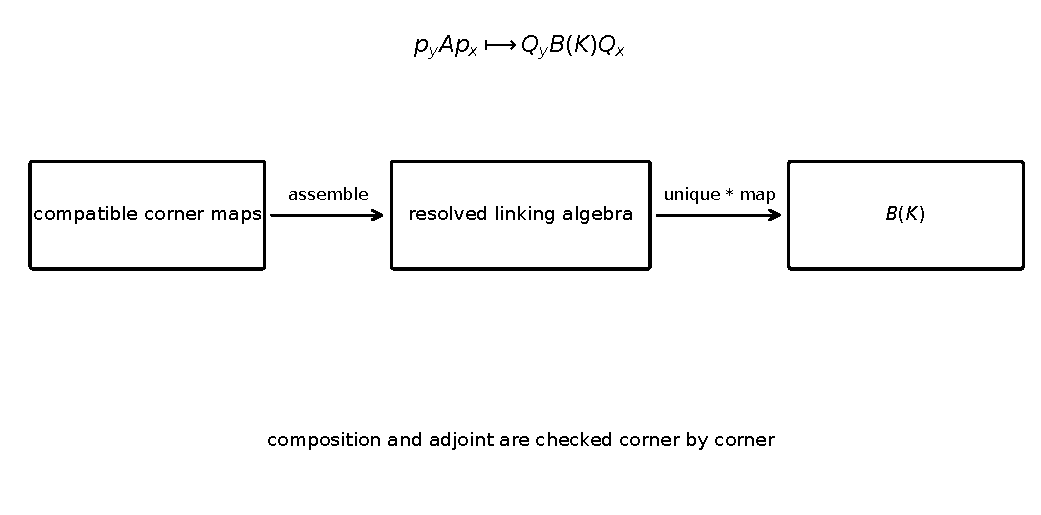
\includegraphics[width=.90\textwidth]{04_linking_universal_property.pdf}
\caption{The linking algebra is universal for compatible corner assignments.}
\label{fig:linking_universal}
\end{figure}

\begin{lemma}[Faithful trace in finite dimension]\label{lem:faithful_trace}
Every finite dimensional \(C^*\) algebra has a faithful tracial state.
\end{lemma}

\begin{proof}
Write
\[
 A\cong\bigoplus_{r=1}^{m}M_{n_r}(\CC).
\]
Choose positive numbers \(c_r\) with sum one and define
\[
 \tau(a_1,\ldots,a_m)
 =
 \sum_{r=1}^{m}c_r\frac{\Tr(a_r)}{n_r}.
\]
This is tracial and positive. If \(a\ne0\), then some block of \(a^*a\) is nonzero positive, so \(\tau(a^*a)>0\).
\end{proof}

\begin{theorem}[Faithful left regular representation]\label{thm:left_regular}
Let \(A\) be finite dimensional and let \(\tau\) be a faithful tracial state. Equip \(A\) with
\[
 \langle a,b\rangle_\tau=\tau(a^*b).
\]
Left multiplication
\[
 \lambda(x)a=xa
\]
defines a faithful unital star representation
\[
 \lambda:A\longrightarrow\B(L^2(A,\tau)).
\]
\end{theorem}

\begin{proof}
Associativity gives multiplicativity and \(\lambda(1)=I\). The trace property gives
\[
 \langle\lambda(x)a,b\rangle_\tau
 =
 \tau(a^*x^*b)
 =
 \langle a,\lambda(x^*)b\rangle_\tau.
\]
If \(\lambda(x)=0\), then \(x=\lambda(x)1=0\).
\end{proof}

\begin{theorem}[Universal projector corner representation]\label{thm:universal_projector_representation}
Every unital resolved linking system admits a Hilbert space \(H\) and a faithful unital star representation
\[
 \pi:A\longrightarrow\B(H)
\]
such that
\[
 P_x=\pi(p_x)
\]
form a complete orthogonal family, the packet elements
\[
 B_{x,i}=\pi(e_{x,i})
\]
form orthogonal subprojectors resolving \(P_x\), and
\[
 \pi(p_yAp_x)=P_y\pi(A)P_x,
\]
\[
 \pi(e_{y,a}Ae_{x,i})
 =
 B_{y,a}\pi(A)B_{x,i}.
\]
Every declared refinement is preserved exactly.
\end{theorem}

\begin{proof}
The Gelfand Naimark theorem gives a faithful unital star representation of \(A\) \Rcite{R1}. Star homomorphisms carry projections to projections, preserve products, and preserve finite sums. The object and packet relations from \cref{def:resolved_linking_system} therefore become orthogonal projector relations. Faithfulness gives both corner equalities. If
\[
 e=\sum_\alpha e_\alpha
\]
is a declared refinement, then
\[
 \pi(e)=\sum_\alpha\pi(e_\alpha)
\]
with orthogonal summands.
\end{proof}

\begin{corollary}[Resolved \(C^*\) categories]\label{cor:resolved_categories}
Every finite resolved \(C^*\) category whose standard linking algebra is formed from its hom spaces has a faithful concrete realization by Hilbert spaces and projector corners.
\end{corollary}

\begin{proof}
Apply \cref{thm:universal_projector_representation} to the linking algebra. Object identities become object projectors and hom spaces become the corresponding corners.
\end{proof}

\begin{theorem}[Recognition theorem]\label{thm:recognition}
Consider the following constructions.
\begin{enumerate}
\item Represent a resolved linking system faithfully and retain its concrete object and packet projectors.
\item Start from a concrete projector corner system and forget the ambient coordinates while retaining the \(C^*\) algebra, its named projections, corners, and refinement relations.
\end{enumerate}
Every abstract resolved linking system is isomorphic to the system recovered from any faithful concrete realization. Conversely, every concrete projector corner system defines a resolved linking system.
\end{theorem}

\begin{proof}
A concrete system plainly satisfies the axioms. For the other direction, a faithful representation identifies \(A\) with the concrete \(C^*\) algebra \(\pi(A)\). It sends every named projection and every refinement equation to its concrete counterpart. Forgetting coordinates therefore recovers an isomorphic resolved system.
\end{proof}

\begin{proposition}[Refinement naturality]\label{prop:refinement_naturality}
Let
\[
 e=\sum_{\alpha=1}^{r}e_\alpha
\]
be a finite orthogonal refinement in a resolved linking system. Under every unital star representation,
\[
 \pi(e)=\sum_{\alpha=1}^{r}\pi(e_\alpha),
 \qquad
 \pi(e_\alpha)\pi(e_\beta)
 =
 \delta_{\alpha\beta}\pi(e_\alpha).
\]
\end{proposition}

\begin{proof}
A star homomorphism preserves sums, products, adjoints, and zero.
\end{proof}

\begin{figure}[t]
\centering
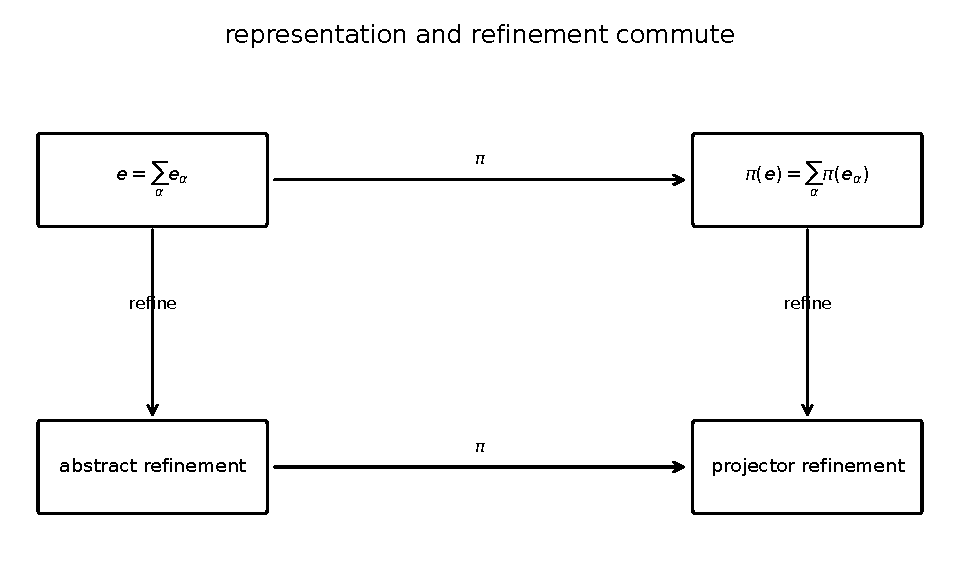
\includegraphics[width=.83\textwidth]{05_refinement_naturality.pdf}
\caption{The abstract and concrete refinement diagrams commute.}
\label{fig:refinement_naturality}
\end{figure}

\begin{theorem}[Minimal faithful dimension in finite dimension]\label{thm:minimal_dimension}
Let
\[
 A\cong\bigoplus_{r=1}^{m}M_{n_r}(\CC).
\]
The smallest Hilbert space dimension of a faithful star representation is
\[
 \boxed{
 \sum_{r=1}^{m}n_r.
 }
\]
The left regular representation acts on a space of dimension
\[
 \sum_{r=1}^{m}n_r^2.
\]
\end{theorem}

\begin{proof}
A faithful representation must contain a nonzero copy of the defining irreducible representation of every simple matrix block, which gives the lower bound. Their direct sum is faithful and attains it. The dimension of the algebra as a Hilbert space is the sum of the squared block sizes.
\end{proof}

\begin{theorem}[Universal GNS realization]\label{thm:universal_gns}
Let \(A\) be a unital \(C^*\) algebra with a finite resolved projection family. The direct sum of the GNS representations over all states of \(A\) is faithful and satisfies the conclusions of \cref{thm:universal_projector_representation}.
\end{theorem}

\begin{proof}
States separate the positive cone. If \(a\ne0\), then \(a^*a\ne0\), so there is a state \(\omega\) with \(\omega(a^*a)>0\). In the GNS representation,
\[
 \norm{\pi_\omega(a)[1]}^2
 =
 \omega(a^*a)>0.
\]
The direct sum over all states is therefore faithful. Projection and refinement preservation follow from the star representation laws.
\end{proof}

\begin{proposition}[Monoidal enhancement boundary]\label{prop:monoidal_boundary}
Let \(\Ccal\) be a resolved monoidal \(C^*\) category. A concrete realization preserving the tensor product through coherent unitary isomorphisms is exactly a faithful unitary strong monoidal star functor
\[
 F:\Ccal\longrightarrow\mathrm{Hilb}.
\]
Ordinary corner representability does not by itself supply such a functor.
\end{proposition}

\begin{proof}
A tensor preserving concrete realization assigns Hilbert spaces to objects, bounded maps to morphisms, and coherent unitaries
\[
 F(X)\otimes F(Y)\cong F(X\otimes Y)
\]
compatible with associativity, units, dagger, and composition. This is precisely a unitary strong monoidal star functor. The converse is immediate from the definition.
\end{proof}

\section{Weighted transfer algebras and inverse packet paths}\label{sec:weighted_inverse}

A resolution is most useful when transfer blocks decay with packet distance or interaction complexity. Weighted block algebras record that decay. The local inverse mechanism is the packet analogue of classical Wiener inversion \Rcite{R18}. The finite theory below extends without change to countable packet families whenever the defining row and column sums are finite.

\begin{definition}[Admissible packet weight]\label{def:admissible_weight}
Let \(I\) be a packet set. An admissible weight is a symmetric function
\[
 w:I\times I\longrightarrow[1,\infty)
\]
satisfying
\[
 w(i,i)=1,
 \qquad
 w(k,i)\leq w(k,j)w(j,i).
\]
For a block transfer \(T=(T_{ai})\), define
\[
 \norm T_{w,c}
 =
 \sup_i\sum_a w(a,i)\norm{T_{ai}},
\]
\[
 \norm T_{w,r}
 =
 \sup_a\sum_i w(a,i)\norm{T_{ai}},
\]
and
\[
 \norm T_{\mathfrak S_w}
 =
 \max\{\norm T_{w,c},\norm T_{w,r}\}.
\]
\end{definition}

\begin{theorem}[Weighted block Schur algebra]\label{thm:weighted_schur_algebra}
The block families with finite \(\mathfrak S_w\) norm form a Banach star algebra. They act boundedly on the Hilbert direct sum, with
\[
 \boxed{
 \norm T\leq\norm T_{\mathfrak S_w}.
 }
\]
Moreover,
\[
 \boxed{
 \norm{ST}_{\mathfrak S_w}
 \leq
 \norm S_{\mathfrak S_w}\norm T_{\mathfrak S_w},
 \qquad
 \norm{T^*}_{\mathfrak S_w}=\norm T_{\mathfrak S_w}.
 }
\]
\end{theorem}

\begin{proof}
The scalar matrix \((\norm{T_{ai}})\) has uniformly bounded row and column sums, so the Schur test gives boundedness on the Hilbert direct sum. For composition,
\[
 \sum_cw(c,i)\norm{(ST)_{ci}}
 \leq
 \sum_{c,a}w(c,a)\norm{S_{ca}}w(a,i)\norm{T_{ai}}.
\]
Taking the column supremum gives the product bound. The row estimate is identical. Symmetry of \(w\) gives the adjoint identity. Completeness follows by blockwise convergence and Fatou's inequality for the row and column sums.
\end{proof}

\begin{theorem}[Local resolved Wiener theorem]\label{thm:resolved_neumann_inverse}
If \(A\in\mathfrak S_w\) and
\[
 \norm{I-A}_{\mathfrak S_w}<1,
\]
then \(A\) is invertible in the same weighted transfer algebra and
\[
 \boxed{
 A^{-1}
 =
 \sum_{n=0}^{\infty}(I-A)^n,
 \qquad
 \norm{A^{-1}}_{\mathfrak S_w}
 \leq
 \frac1{1-\norm{I-A}_{\mathfrak S_w}}.
 }
\]
\end{theorem}

\begin{proof}
This is the Neumann series in the Banach algebra from \cref{thm:weighted_schur_algebra}.
\end{proof}

Let \(T=D+R\), where \(D\) is block diagonal and every diagonal block is invertible. Let \(D^{-1}\) denote the block diagonal inverse.

\begin{theorem}[Block diagonal inverse path expansion]\label{thm:block_inverse_paths}
If
\[
 \rho=\norm{D^{-1}R}_{\mathfrak S_w}<1,
\]
then
\[
 \boxed{
 T^{-1}
 =
 \sum_{n=0}^{\infty}
 (-D^{-1}R)^nD^{-1}.
 }
\]
The block from packet \(i\) to packet \(a\) is the absolutely convergent sum over packet paths
\[
 \boxed{
 (T^{-1})_{ai}
 =
 \sum_{n\geq0}(-1)^n
 \sum_{i=i_0,\ldots,i_n=a}
 D_a^{-1}R_{a i_{n-1}}D_{i_{n-1}}^{-1}
 \cdots
 R_{i_1i}D_i^{-1}.
 }
\]
The weighted norm satisfies
\[
 \norm{T^{-1}}_{\mathfrak S_w}
 \leq
 \frac{\norm{D^{-1}}_{\mathfrak S_w}}{1-\rho}.
\]
\end{theorem}

\begin{proof}
Factor
\[
 T=D(I+D^{-1}R)
\]
and apply \cref{thm:resolved_neumann_inverse}. Matrix multiplication expands the \(n\)th power as the sum over all packet paths of length \(n\).
\end{proof}

\begin{corollary}[Off diagonal inverse decay]\label{cor:inverse_decay}
Suppose the packet set carries a metric \(d\) and
\[
 w(a,i)=e^{\alpha d(a,i)}.
\]
Under the hypotheses of \cref{thm:block_inverse_paths},
\[
 \boxed{
 \norm{(T^{-1})_{ai}}
 \leq
 e^{-\alpha d(a,i)}
 \frac{\norm{D^{-1}}_{\mathfrak S_w}}{1-\rho}.
 }
\]
\end{corollary}

\begin{proof}
Every block is bounded by its weighted norm divided by \(w(a,i)\).
\end{proof}

\begin{figure}[t]
\centering
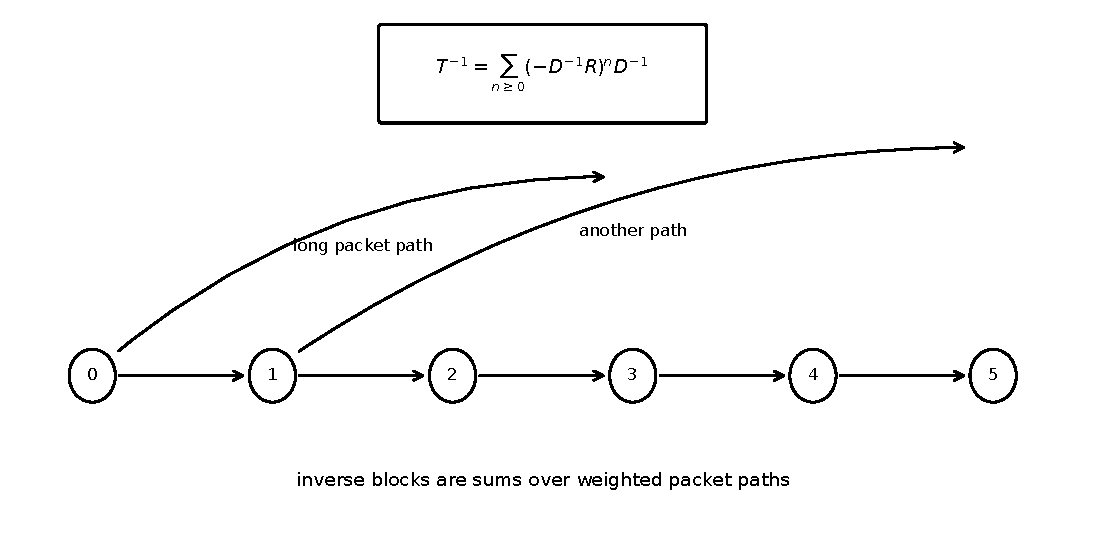
\includegraphics[width=.90\textwidth]{18_weighted_inverse_paths.pdf}
\caption{The inverse of a block dominant transfer is a convergent sum over packet paths. Admissible weights convert path length into off diagonal decay.}
\label{fig:weighted_inverse_paths}
\end{figure}

\begin{proposition}[Two packet Schur complement]\label{prop:schur_complement}
Let
\[
 T=
 \begin{pmatrix}
 A&B\\
 C&D
 \end{pmatrix}
\]
relative to a two packet resolution. If \(D\) and
\[
 S=A-BD^{-1}C
\]
are invertible, then
\[
 \boxed{
 T^{-1}
 =
 \begin{pmatrix}
 S^{-1}&-S^{-1}BD^{-1}\\
 -D^{-1}CS^{-1}&D^{-1}+D^{-1}CS^{-1}BD^{-1}
 \end{pmatrix}.
 }
\]
The correction \(BD^{-1}C\) is the exact transfer through the eliminated packet.
\end{proposition}

\begin{proof}
Multiply the displayed matrix by \(T\) on both sides and use the definition of \(S\).
\end{proof}

\begin{remark}[Global inverse closure boundary]\label{rem:global_weighted_boundary}
The local Neumann theorem proves inverse closure near an invertible diagonal or near the identity. It does not prove that every invertible element of an arbitrary weighted transfer algebra has a weighted inverse. That stronger spectral invariance problem remains in \cref{sec:boundaries}.
\end{remark}

\section{Countable, unbounded, and normal completion}\label{sec:countable}

Finite resolutions sum in norm because every sum is finite. Countable resolutions require a declared topology. Inductive limit constructions provide a complementary route to infinite operator algebras \Rcite{R11}. In Hilbert space, orthogonal packet sums naturally converge strongly. Norm convergence returns for compact and Schatten class operators. Unbounded generators require domains, graph norms, forms, or bounded surrogates. The categorical background for countable direct sums and \(W^*\) categories is developed in \Rcite{R2}, \Rcite{R5}, while Hilbert \(C^*\) module and unbounded operator techniques are treated in \Rcite{R6}, \Rcite{R7}, \Rcite{R10}, and \Rcite{R20}.

\subsection{Countable orthogonal resolutions}

\begin{definition}[Countable Hilbert resolution]\label{def:countable_resolution}
A countable Hilbert resolution of \(\Hh\) is a family of mutually orthogonal projections \((P_n)_{n\ge1}\) such that
\[
 \sum_{n\ge1}P_n=I
\]
in the strong operator topology. For a finite set \(F\subset\NN\), put
\[
 P_F=\sum_{n\in F}P_n.
\]
\end{definition}

\begin{lemma}[Strong convergence of packet sums]\label{lem:strong_packet_sum}
For a countable Hilbert resolution,
\[
 P_Fx\longrightarrow x
\]
for every \(x\in\Hh\), and
\[
 \norm{x}^2
 =
 \sum_{n\ge1}\norm{P_nx}^2.
\]
\end{lemma}

\begin{proof}
The packet ranges are orthogonal. Their closed linear span is all of \(\Hh\) by strong completeness. The usual orthogonal expansion theorem gives both claims.
\end{proof}

\begin{theorem}[Strong packet reconstruction]\label{thm:strong_reconstruction}
Let \((Q_i)\) resolve \(\K\) and \((P_j)\) resolve \(\Hh\). For every bounded \(T:\Hh\to\K\),
\[
 \boxed{
 T
 =
 \operatorname*{s\!\!\lim}_{F,G}
 Q_FTP_G.
 }
\]
The same holds for \(T^*\), so the convergence is strong star.
\end{theorem}

\begin{proof}
For finite \(F,G\),
\[
 T-Q_FTP_G
 =
 (I-Q_F)T+Q_FT(I-P_G).
\]
Applied to a fixed vector \(x\), the first term tends to zero because \(Q_F\to I\) strongly on \(\K\), and the second tends to zero because \(P_Gx\to x\). Apply the same argument to \(T^*\).
\end{proof}

\begin{theorem}[Compact and Schatten truncation]\label{thm:compact_truncation}
If \(T:\Hh\to\K\) is compact, then
\[
 \norm{T-Q_GTP_F}\longrightarrow0.
\]
If \(T\) belongs to the Schatten ideal \(S_p\), \(1\le p<\infty\), then
\[
 \norm{T-Q_GTP_F}_{S_p}\longrightarrow0.
\]
For \(p=2\),
\[
 \boxed{
 \norm{T}_{\mathrm{HS}}^2
 =
 \sum_{i,j\ge1}\norm{Q_iTP_j}_{\mathrm{HS}}^2.
 }
\]
\end{theorem}

\begin{proof}
Strong convergence of bounded projections is uniform on compact subsets. Apply this to the compact image of the unit ball under \(T\) and to \(T^*\). This proves operator norm convergence. Finite rank operators are dense in every \(S_p\), and the truncation maps are contractions on \(S_p\). The Hilbert Schmidt identity follows from orthogonality of the corners \Rcite{R9}.
\end{proof}

\begin{figure}[t]
\centering
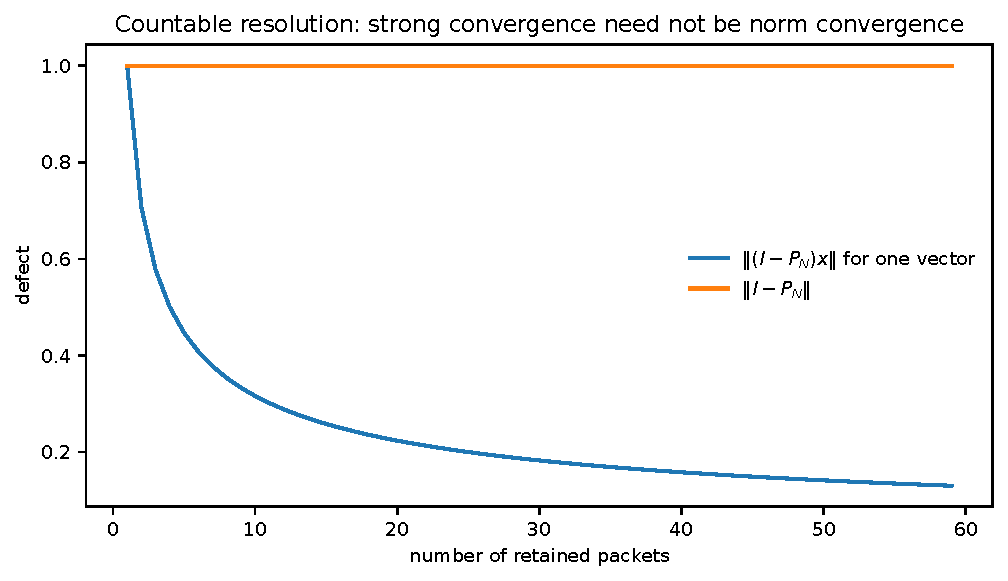
\includegraphics[width=.75\textwidth]{06_strong_vs_norm.pdf}
\caption{Countable packet sums converge strongly even when the operator norm defect remains one.}
\label{fig:strong_vs_norm}
\end{figure}

\begin{theorem}[Countable packet path composition]\label{thm:countable_path}
Let \(T:\Hh\to\K\) and \(S:\K\to\Lcal\) be bounded. For countable resolutions \((P_k)\), \((Q_j)\), and \((R_i)\),
\[
 R_iSTP_kx
 =
 \sum_{j\ge1}R_iSQ_jTP_kx
\]
for every \(x\in P_k\Hh\), with convergence in \(R_i\Lcal\).
\end{theorem}

\begin{proof}
The partial sums \(\sum_{j\in F}Q_jTP_kx\) converge to \(TP_kx\). The bounded map \(R_iS\) preserves norm convergence.
\end{proof}

\subsection{Countable resolved categories}

\begin{definition}[Countably resolved \(C^*\) category]\label{def:countably_resolved_category}
A countably resolved \(C^*\) category is a small \(C^*\) category with countable object set, together with a countable orthogonal family of packet projections in every endomorphism algebra whose supremum is the object identity, and a declared family of compatible refinements.
\end{definition}

\begin{theorem}[Countable linking representation]\label{thm:countable_linking}
Let \(\Ccal\) be a countable small \(C^*\) category and let \(F\) be a faithful nondegenerate star functor to Hilbert spaces. Form the norm closure \(L(\Ccal)\) of finite support operator matrices on the Hilbert direct sum of the object spaces. Then
\begin{enumerate}
\item \(L(\Ccal)\) is sigma unital.
\item Every object projection belongs to the multiplier algebra \(M(L(\Ccal))\).
\item
\[
 P_yL(\Ccal)P_x
 =
 F(\Ccal(x,y)).
\]
\item Finite sums of object projections form an approximate identity.
\item Countable packet projections sum strongly to the object projection.
\end{enumerate}
\end{theorem}

\begin{proof}
Finite support matrices form a star algebra. Their norm closure is a \(C^*\) algebra. Enumerate the objects and let \(E_N\) be the sum of the first \(N\) object projections. Multiplication by \(E_N\) eventually fixes every finite support matrix, so \((E_N)\) is an approximate identity.

Every object projection multiplies finite support matrices into finite support matrices on both sides, hence defines a multiplier. Faithfulness of a \(C^*\) functor is isometric on each hom space, so the represented hom space is closed and equals the corresponding corner. Strong orthogonal summation gives the packet conclusion.
\end{proof}

\begin{theorem}[Nondegenerate factorization]\label{thm:nondegenerate_factorization}
Nondegenerate star representations of \(L(\Ccal)\) are equivalent, up to unitary equivalence, to nondegenerate star functors from \(\Ccal\) to Hilbert spaces. The multiplier extensions of the object projections recover the object Hilbert spaces.
\end{theorem}

\begin{proof}
Given a nondegenerate representation, extend it strictly to the multiplier algebra and take the ranges of the object projections as object spaces. Corners act as the categorical morphisms. Conversely, a nondegenerate functor acts on the Hilbert direct sum of its object spaces, and finite operator matrices extend to the linking algebra. The two constructions are inverse up to the canonical unitary identification.
\end{proof}

\begin{theorem}[Normal preservation of countable packet joins]\label{thm:normal_joins}
Let \(F\) be a faithful normal star functor between resolved \(W^*\) categories. For every increasing sequence of packet projections,
\[
 F\left(\bigvee_np_n\right)
 =
 \bigvee_nF(p_n).
\]
The analogous statement holds for decreasing meets.
\end{theorem}

\begin{proof}
Normality is ultraweak continuity on bounded increasing nets of positive operators. The join of an increasing sequence of projections is its strong and ultraweak limit. Meets follow from complements \Rcite{R2}, \Rcite{R8}.
\end{proof}

\subsection{Unbounded generators}

\begin{definition}[Reducing packet for an unbounded operator]\label{def:unbounded_reduction}
Let \(D\) be a closed densely defined operator. A projection \(P\) reduces \(D\) if
\[
 P\operatorname{Dom}(D)\subseteq\operatorname{Dom}(D)
\]
and
\[
 DPx=PDx
 \qquad
 (x\in\operatorname{Dom}(D)),
\]
with the same property for \(I-P\).
\end{definition}

\begin{theorem}[Unbounded direct sum decomposition]\label{thm:unbounded_direct_sum}
Let \(D\) be self adjoint and let \((P_n)\) be a countable resolution reducing \(D\). Put
\[
 \Hh_n=P_n\Hh,
 \qquad
 D_n=D|_{\operatorname{Dom}(D)\cap\Hh_n}.
\]
Then every \(D_n\) is self adjoint and
\[
 \boxed{
 D=\bigoplus_{n\ge1}D_n.
 }
\]
For every bounded Borel function \(f\),
\[
 f(D)
 =
 \operatorname*{s\!\!\sum}_{n\ge1}
 P_nf(D)P_n.
\]
\end{theorem}

\begin{proof}
Reduction implies commutation with the resolvent and hence with the spectral measure. Every packet range is therefore a reducing spectral subspace. The spectral theorem gives the direct sum and functional calculus statements \Rcite{R10}, \Rcite{R20}.
\end{proof}

\begin{theorem}[Graph norm reconstruction]\label{thm:graph_norm}
Under the hypotheses of \cref{thm:unbounded_direct_sum}, if
\[
 P^{(N)}=\sum_{n=1}^{N}P_n,
\]
then for every \(x\in\operatorname{Dom}(D)\),
\[
 \norm{x-P^{(N)}x}_D\longrightarrow0,
\]
where
\[
 \norm{x}_D^2=\norm{x}^2+\norm{Dx}^2.
\]
Moreover,
\[
 \norm{x}_D^2
 =
 \sum_{n\ge1}
 \left(
 \norm{P_nx}^2+\norm{DP_nx}^2
 \right).
\]
\end{theorem}

\begin{proof}
The vectors \(P_nx\) are orthogonal. Since the projectors commute with \(D\) on its domain, the vectors \(DP_nx=P_nDx\) are also orthogonal. Apply Parseval to \(x\) and to \(Dx\).
\end{proof}

Define the resolvent and bounded transform
\[
 R_z(D)=(D-zI)^{-1},
 \qquad
 F_D=D(1+D^2)^{-1/2}.
\]

\begin{theorem}[Bounded surrogate packetization]\label{thm:bounded_surrogate}
If a projection \(P\) reduces a self adjoint \(D\), then \(P\) commutes with every resolvent, with \(F_D\), and with every bounded Borel function of \(D\). Conversely, commutation with one nonreal resolvent implies reduction of \(D\).
\end{theorem}

\begin{proof}
Reduction gives commutation with the spectral measure and hence with functional calculus. Conversely, if \(P\) commutes with \(R_z(D)\), then it preserves the range of the resolvent, which is \(\operatorname{Dom}(D)\), and commutes there with
\[
 D=zI+R_z(D)^{-1}.
\]
\end{proof}

\begin{theorem}[Resolvent commutator identity]\label{thm:resolvent_commutator}
Suppose \(P\) preserves \(\operatorname{Dom}(D)\) and \([D,P]\) extends to a bounded operator. For \(z\notin\RR\),
\[
 \boxed{
 [P,R_z(D)]
 =
 R_z(D)[D,P]R_z(D).
 }
\]
Consequently,
\[
 \boxed{
 \norm{[P,R_z(D)]}
 \le
 \frac{\norm{[D,P]}}{\abs{\operatorname{Im}z}^2}.
 }
\]
\end{theorem}

\begin{proof}
Apply the inverse commutator identity to \(D-zI\). The spectral theorem gives
\[
 \norm{R_z(D)}\le\abs{\operatorname{Im}z}^{-1}.
\]
\end{proof}

\begin{figure}[t]
\centering
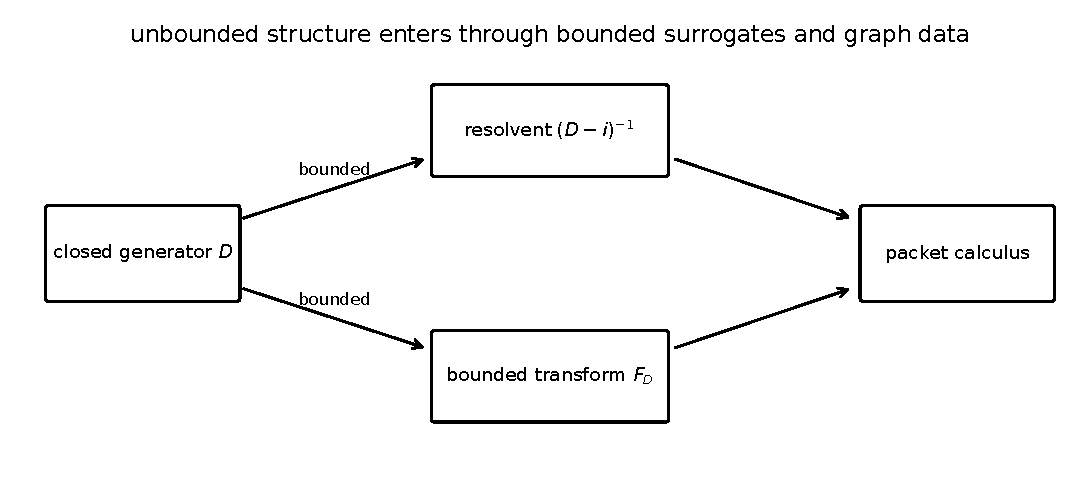
\includegraphics[width=.94\textwidth]{07_unbounded_completion.pdf}
\caption{Unbounded generators enter the bounded packet calculus through resolvents, bounded transforms, spectral projections, and graph data.}
\label{fig:unbounded_completion}
\end{figure}

\subsection{Measurable packet fields}

\begin{theorem}[Decomposable packet reconstruction]\label{thm:decomposable_reconstruction}
Let
\[
 T=\int_X^{\oplus}T(x)\,d\mu(x)
\]
be a bounded decomposable operator. Let
\[
 P_n=\int_X^{\oplus}P_n(x)\,d\mu(x)
\]
be measurable orthogonal projection fields with strong sum equal to the identity almost everywhere. Then
\[
 \boxed{
 T
 =
 \operatorname*{s\!\!\sum}_{m,n}P_mTP_n,
 }
\]
and every block is decomposable:
\[
 P_mTP_n
 =
 \int_X^{\oplus}P_m(x)T(x)P_n(x)\,d\mu(x).
\]
Moreover,
\[
 \norm{T}
 =
 \operatorname*{ess\,sup}_{x\in X}\norm{T(x)}.
\]
\end{theorem}

\begin{proof}
The statements hold fiberwise. Measurability and essential boundedness make the block fields decomposable. Fiberwise strong reconstruction and dominated convergence give the global strong sum. The norm identity is the standard decomposable operator formula \Rcite{R8}.
\end{proof}

\begin{theorem}[Countable and unbounded completion]\label{thm:countable_completion}
Let \(\Ccal\) be a countable resolved \(C^*\) category with countable orthogonal packet families. After faithful nondegenerate representation, closure under countable Hilbert direct sums, splitting of packet idempotents, and normal completion, the following hold.
\begin{enumerate}
\item The bounded part is a countably additive resolved \(C^*\) category.
\item Packet objects form its resolved Karoubi envelope.
\item The countable linking algebra represents finite support transfers and their norm limits.
\item Object and packet projections act as multipliers and sum strongly.
\item The normal completion is a resolved \(W^*\) category in which countable packet joins are preserved.
\item Reduced self adjoint generators define affiliated packet objects through graph domains, resolvents, and bounded transforms.
\item Certified finite sections converge in the topology appropriate to the represented object.
\end{enumerate}
\end{theorem}

\begin{proof}
Countable direct sums supply the additive completion. Splitting projections gives the Karoubi envelope. \Cref{thm:countable_linking,thm:nondegenerate_factorization} give the linking representation and multiplier structure. \Cref{thm:normal_joins} gives normal completion. \Cref{thm:unbounded_direct_sum,thm:graph_norm,thm:bounded_surrogate} give the unbounded part. The convergence statements follow from \cref{thm:strong_reconstruction,thm:compact_truncation,thm:decomposable_reconstruction}.
\end{proof}

\subsection{Normal states, strict windows, and packet objects}

\begin{theorem}[Trace class packet truncation]\label{thm:trace_state_truncation}
Let \(\rho\geq0\) be trace class with \(\Tr\rho=1\), and let \((P_n)\) be a countable resolution. Put
\[
 P^{(N)}=\sum_{n=1}^{N}P_n,
 \qquad
 m_N=\Tr(P^{(N)}\rho).
\]
Then
\[
 \boxed{
 \norm{\rho-P^{(N)}\rho P^{(N)}}_1\longrightarrow0.
 }
\]
If \(m_N>0\), the normalized finite state
\[
 \rho_N=\frac{P^{(N)}\rho P^{(N)}}{m_N}
\]
also converges to \(\rho\) in trace norm.
\end{theorem}

\begin{proof}
Finite rank operators are dense in the trace class, and multiplication by a projection is contractive in trace norm. Hence the unnormalized truncations converge. Since \(m_N\to1\),
\[
 \norm{\rho_N-\rho}_1
 \leq
 \frac{\norm{P^{(N)}\rho P^{(N)}-\rho}_1}{m_N}
 +
 \left|\frac1{m_N}-1\right|\norm\rho_1,
\]
and both terms tend to zero.
\end{proof}

\begin{theorem}[Strict finite window reconstruction]\label{thm:strict_windows}
Let \(L(\Ccal)\) be a countable linking algebra and let \(E_N\) be the sum of the first \(N\) object projections in its multiplier algebra. Then
\[
 \boxed{
 \norm{E_Na-a}+\norm{aE_N-a}\longrightarrow0
 }
\]
for every \(a\in L(\Ccal)\). Thus \(E_N\to1\) strictly, while norm convergence of \(E_N\) to the multiplier unit generally fails.
\end{theorem}

\begin{proof}
The claim is exact for finite support matrices once the window contains their support. Such matrices are norm dense, and left and right multiplication by \(E_N\) are contractions. Approximation proves strict convergence. Proper projections remain one unit away from the identity in operator norm.
\end{proof}

\begin{definition}[Resolved Karoubi object]\label{def:karoubi_object}
A resolved Karoubi object is a pair \((X,e)\) with
\[
 e=e^*=e^2\in\Ccal(X,X).
\]
A morphism \(a:(X,e)\to(Y,f)\) satisfies \(a=fae\).
\end{definition}

\begin{theorem}[Countable packet splitting]\label{thm:karoubi_packet_splitting}
Let a resolved \(C^*\) category be represented faithfully on Hilbert spaces and completed under countable Hilbert direct sums. If
\[
 e=\operatorname*{s\!\!\sum}_{n\geq1}e_n
\]
is a strong sum of mutually orthogonal packet projections on the represented object \(X\), then the represented Karoubi object \((X,e)\) is unitarily isomorphic to the Hilbert direct sum
\[
 \boxed{
 (X,e)\cong\bigoplus_{n\geq1}(X,e_n).
 }
\]
\end{theorem}

\begin{proof}
The ranges \(e_nX\) are mutually orthogonal, and their closed linear span is \(eX\) because the projector sum is strong. The map
\[
 eX\longrightarrow\bigoplus_ne_nX,
 \qquad
 x\longmapsto(e_nx)_n
\]
is unitary by Parseval. Its adjoint synthesizes a square summable packet family by orthogonal summation. These maps are the inclusion and projection morphisms of the countable direct sum.
\end{proof}

\begin{figure}[t]
\centering
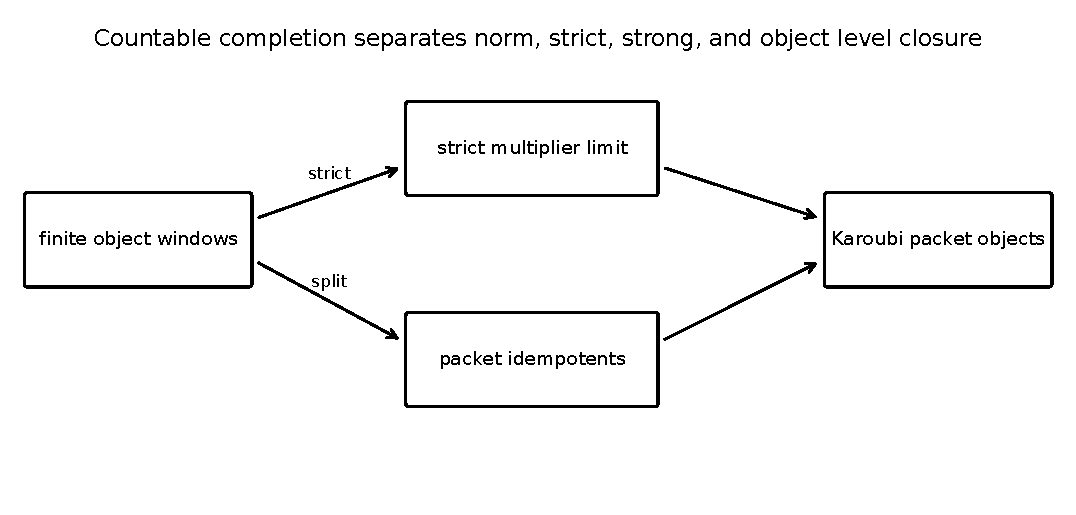
\includegraphics[width=.89\textwidth]{19_strict_karoubi.pdf}
\caption{Countable completion has distinct norm, strict, strong, and object splitting layers. Each topology solves a different reconstruction problem.}
\label{fig:strict_karoubi}
\end{figure}

\begin{theorem}[Expanded categorical completion]\label{thm:expanded_categorical_completion}
Let \(\Ccal\) be a countable resolved \(C^*\) category with countable orthogonal packet families. Assume a faithful nondegenerate representation and close the represented system under countable Hilbert direct sums and split packet idempotents. Then
\begin{enumerate}
\item the bounded part is countably additive
\item the packet objects form the resolved Karoubi envelope
\item the countable linking algebra is recovered by norm limits of finite support windows
\item object windows converge strictly in the multiplier algebra
\item normal completion gives a resolved \(W^*\) category preserving countable packet joins
\item trace class states are recovered in trace norm by normalized packet windows.
\end{enumerate}
\end{theorem}

\begin{proof}
Countable direct sums give the additive completion. \Cref{thm:karoubi_packet_splitting} gives the Karoubi envelope. \Cref{thm:countable_linking,thm:strict_windows} give the linking and multiplier statements. \Cref{thm:normal_joins} gives normal completion, and \cref{thm:trace_state_truncation} gives the state statement.
\end{proof}

\subsection{Quadratic forms, resolvent limits, and dynamical leakage}

\begin{theorem}[Form packet reconstruction]\label{thm:form_packet_reconstruction}
Let \(q\) be a densely defined closed nonnegative quadratic form. Suppose a countable resolution preserves \(\Dom(q)\) and is orthogonal for the form inner product
\[
 \langle x,y\rangle_q
 =
 \langle x,y\rangle+q(x,y).
\]
Then
\[
 \boxed{
 \norm{x}_q^2
 =
 \sum_n\norm{P_nx}_q^2,
 }
\]
and the finite packet sums converge in form norm.
\end{theorem}

\begin{proof}
The form domain is a Hilbert space under the form inner product. The declared packets are a complete orthogonal resolution in that Hilbert space, so Parseval applies there.
\end{proof}

\begin{theorem}[Reducing windows converge in strong resolvent sense]\label{thm:strong_resolvent_windows}
Let \(D\) be self adjoint and let \(P_N\uparrow I\) strongly with every \(P_N\) reducing \(D\). Put
\[
 D_N
 =
 D|_{P_N\Hh}\oplus0|_{(I-P_N)\Hh}.
\]
Then \(D_N\to D\) in the strong resolvent topology. Moreover,
\[
 \boxed{
 \norm{e^{-itD}x-e^{-itD}P_Nx}
 =
 \norm{(I-P_N)x}
 }
\]
for every \(t\in\RR\).
\end{theorem}

\begin{proof}
For \(z\notin\RR\),
\[
 (D_N-z)^{-1}x
 =
 P_N(D-z)^{-1}P_Nx-z^{-1}(I-P_N)x.
\]
The first term converges strongly to the resolvent of \(D\), and the second tends to zero. Reduction makes the omitted packet subspace invariant under the unitary group, which gives the norm identity.
\end{proof}

\begin{proposition}[Dynamical leakage from an approximate packet]\label{prop:dynamical_leakage}
Let \(D\) be bounded and self adjoint, and let \(P\) be a projection. Then
\[
 \boxed{
 \norm{(I-P)e^{-itD}P}
 \leq
 |t|\norm{[D,P]}.
 }
\]
The same formula holds for an unbounded self adjoint generator whenever the commutator extends boundedly on the domain.
\end{proposition}

\begin{proof}
Duhamel's formula gives
\[
 (I-P)e^{-itD}P
 =
 -i\int_0^t
 (I-P)e^{-i(t-s)D}[D,P]e^{-isD}P\,ds.
\]
Unitary invariance of the norm gives the estimate.
\end{proof}

\subsection{Measurable chart covariance}

\begin{proposition}[Measurable unitary covariance]\label{prop:measurable_covariance}
In the setting of \cref{thm:decomposable_reconstruction}, let \(U(x)\) be a measurable essentially bounded unitary field. Define
\[
 \widetilde P_n(x)=U(x)P_n(x)U(x)^*,
 \qquad
 \widetilde T(x)=U(x)T(x)U(x)^*.
\]
Then every packet corner transforms covariantly:
\[
 \boxed{
 \widetilde P_m\widetilde T\widetilde P_n
 =
 U(P_mTP_n)U^*.
 }
\]
Thus two measurable charts represent one resolved field whenever they are related by measurable unitary conjugation.
\end{proposition}

\begin{proof}
The identity holds fiberwise almost everywhere and therefore holds for the decomposable direct integral operators.
\end{proof}

\section{Nonlinear resolution by packet jets}\label{sec:nonlinear}

A linear transfer has one input packet. A nonlinear map creates interactions among several input packets. The correct combinatorial object is therefore a typed hypergraph, and the correct composition law is rooted tree substitution. The operadic background is standard \Rcite{R14}. Resolution Theory adds a declared packet hierarchy, weighted block norms, exact refinement, and named residuals.

\subsection{Resolved multilinear maps}

Let \(X\) and \(Y\) be Banach spaces with finite bounded resolutions
\[
 I_X=\sum_{j\in J}P_j,
 \qquad
 I_Y=\sum_{i\in I}Q_i.
\]
Choose positive packet weights \(a_j\) and \(b_i\), and define
\[
 \norm{x}_a
 =
 \max_j\frac{\norm{P_jx}}{a_j},
 \qquad
 \norm{y}_b
 =
 \max_i\frac{\norm{Q_iy}}{b_i}.
\]

\begin{definition}[Resolved multilinear map]\label{def:resolved_multilinear}
For a bounded \(m\) linear map \(A:X^m\to Y\), define
\[
 A_{i\mid j_1,\ldots,j_m}
 =
 Q_iA(P_{j_1}\cdot,\ldots,P_{j_m}\cdot).
\]
The typed tuple
\[
 (j_1,\ldots,j_m)\longrightarrow i
\]
is its packet hyperedge.
\end{definition}

\begin{theorem}[Exact multilinear reconstruction]\label{thm:multilinear_reconstruction}
Every bounded \(m\) linear map satisfies
\[
 \boxed{
 A(x_1,\ldots,x_m)
 =
 \sum_{i,j_1,\ldots,j_m}
 A_{i\mid j_1,\ldots,j_m}
 (P_{j_1}x_1,\ldots,P_{j_m}x_m).
 }
\]
For finite resolutions the sum is finite and exact.
\end{theorem}

\begin{proof}
Insert the source identities in every input slot and the target identity after applying \(A\). Multilinearity expands the result.
\end{proof}

\begin{theorem}[Weighted packet bound]\label{thm:weighted_packet_bound}
Define
\[
 \norm{A}^{(m)}_{a\to b}
 =
 \max_i\frac1{b_i}
 \sum_{j_1,\ldots,j_m}
 \norm{A_{i\mid j_1,\ldots,j_m}}
 \prod_{r=1}^{m}a_{j_r}.
\]
Then
\[
 \boxed{
 \norm{A(x_1,\ldots,x_m)}_b
 \le
 \norm{A}^{(m)}_{a\to b}
 \prod_{r=1}^{m}\norm{x_r}_a.
 }
\]
\end{theorem}

\begin{proof}
Apply the triangle inequality to the exact reconstruction. Use
\[
 \norm{P_jx_r}\le a_j\norm{x_r}_a
\]
and divide by the target weight.
\end{proof}

\begin{figure}[t]
\centering
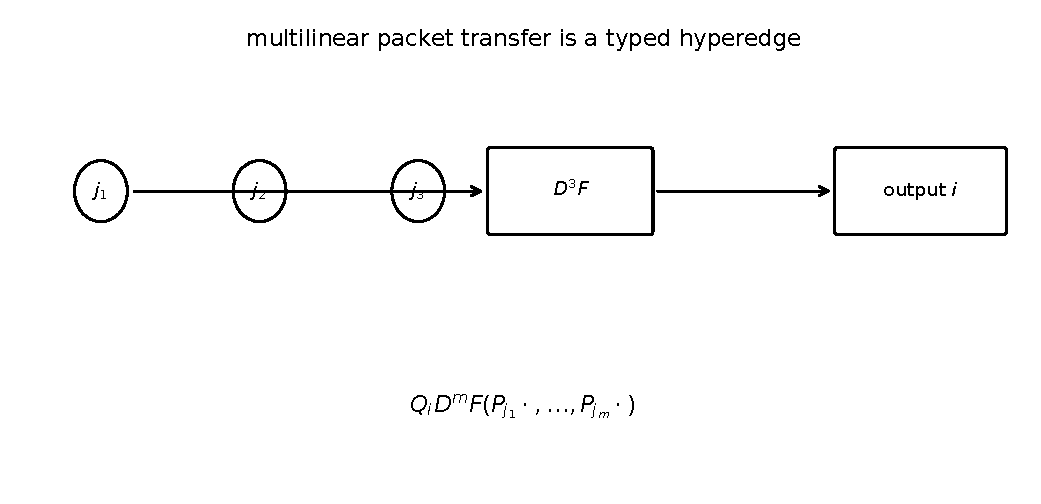
\includegraphics[width=.88\textwidth]{08_nonlinear_hypergraph.pdf}
\caption{A derivative block with several input packets is a typed nonlinear hyperedge.}
\label{fig:nonlinear_hypergraph}
\end{figure}

\subsection{Jets, composition, and refinement}

For a smooth map \(F:X\to Y\), define the packet resolved derivative block
\[
 F^{[m]}_{i\mid j_1,\ldots,j_m}(x)
 =
 Q_iD^mF(x)
 [P_{j_1}\cdot,\ldots,P_{j_m}\cdot].
\]

\begin{theorem}[Packet resolved Faà di Bruno formula]\label{thm:faa_di_bruno}
Let \(X\xrightarrow{F}Y\xrightarrow{G}Z\) be smooth. Let \(\Pi_n\) be the set of partitions of \(\{1,\ldots,n\}\). Then
\[
\begin{aligned}
 D^n(G\circ F)(x)[h_1,\ldots,h_n]
 & =
 \sum_{\pi\in\Pi_n}
 D^{\abs{\pi}}G(F(x))\\
 &\quad\left[
 D^{\abs{A_1}}F(x)[h_r]_{r\in A_1},
 \ldots,
 D^{\abs{A_{\abs{\pi}}}}F(x)
 [h_r]_{r\in A_{\abs{\pi}}}
 \right].
\end{aligned}
\]
After inserting source, intermediate, and target projectors, every summand becomes a rooted tree of packet hyperedges summed over intermediate packet labels.
\end{theorem}

\begin{proof}
The Banach space Faà di Bruno formula gives the partition sum. Insert complete packet resolutions before and after every derivative. Multilinearity expands every identity. The blocks of the partition describe the inner vertices, and the outer derivative joins their outputs.
\end{proof}

\begin{proposition}[Colored symmetric operad]\label{prop:colored_operad}
Take packet spaces as colors and continuous multilinear packet maps as operations. Permutations of inputs give the symmetric actions, identity maps give the units, and rooted tree substitution gives composition. These data satisfy the colored symmetric operad axioms.
\end{proposition}

\begin{proof}
Associativity is associativity of substitution of multilinear maps. Identity maps are units. Permutation compatibility is inherited from the symmetric group action on input slots. Packet labels only type the allowed sources and targets \Rcite{R14}.
\end{proof}

\begin{figure}[t]
\centering
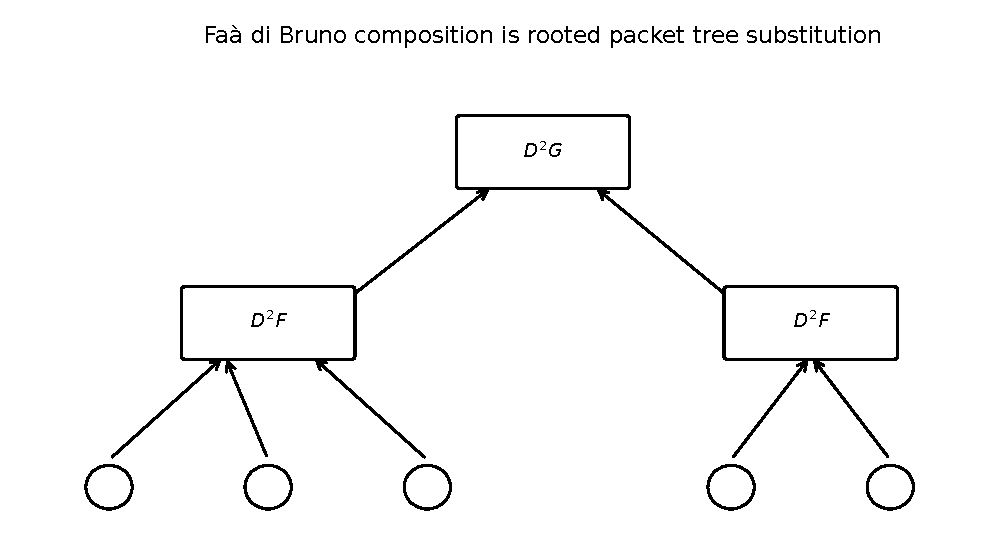
\includegraphics[width=.84\textwidth]{09_operad_composition.pdf}
\caption{Nonlinear composition is rooted packet tree substitution.}
\label{fig:operad_composition}
\end{figure}

\begin{theorem}[Nonlinear refinement coherence]\label{thm:nonlinear_refinement}
Refining the packet jets of \(F\) and \(G\), composing at the refined level, and coarsening gives the same jet as composing first and resolving at the coarse level.
\end{theorem}

\begin{proof}
Both procedures insert complete resolutions of the identity into the same Faà di Bruno formula. The refined calculation retains descendant labels until the final coarsening. The coarse calculation performs those sums immediately. Finite distributivity makes the results equal.
\end{proof}

\begin{proposition}[No free refinement]\label{prop:no_free_refinement}
If every refined hyperedge is active and every contribution must be evaluated, refinement does not reduce the exact arithmetic count. Computational gain requires vanished blocks, low rank, repeated coefficients, selective outputs, transform structure, or reuse.
\end{proposition}

\begin{proof}
Every scalar coefficient of the coarse tensor belongs to exactly one refined block. Summing the sizes of all refined blocks therefore reproduces the original coefficient count.
\end{proof}

\subsection{Analytic packet maps and inversion}

Let
\[
 F(x)=\sum_{m\ge0}A_m[x,\ldots,x]
\]
be analytic on a packet ball, where \(A_m\) is symmetric and \(m\) linear. Define the scalar majorant
\[
 \mathfrak m_F(t)
 =
 \sum_{m\ge0}\norm{A_m}^{(m)}t^m.
\]

\begin{theorem}[Analytic composition bound]\label{thm:analytic_composition}
If \(F(0)=0\) and \(\mathfrak m_F(t)\) lies in the convergence interval of \(\mathfrak m_G\), then
\[
 \boxed{
 \mathfrak m_{G\circ F}(t)
 \le
 \mathfrak m_G(\mathfrak m_F(t)).
 }
\]
\end{theorem}

\begin{proof}
Apply \cref{thm:weighted_packet_bound} to every rooted tree in \cref{thm:faa_di_bruno}. After taking norms, all coefficients are nonnegative. Grouping by total degree gives the scalar majorant composition, with cancellation removed.
\end{proof}

\begin{theorem}[Near identity nonlinear inverse]\label{thm:near_identity_inverse}
Let
\[
 F=I+N,
 \qquad
 N(0)=0.
\]
Assume that on the packet ball \(B_R\),
\[
 \kappa
 =
 \sup_{x\in B_R}\norm{DN(x)}<1.
\]
For every \(y\) with
\[
 \norm{y}\le(1-\kappa)R,
\]
there is a unique \(x\in B_R\) such that \(F(x)=y\). The inverse \(H=F^{-1}\) is analytic on the resulting neighborhood, and
\[
 DH(y)
 =
 [I+DN(H(y))]^{-1}
 =
 \sum_{q=0}^{\infty}[-DN(H(y))]^q.
\]
\end{theorem}

\begin{proof}
For fixed \(y\), define \(\Psi_y(x)=y-N(x)\). The derivative bound makes \(\Psi_y\) a contraction with constant \(\kappa\). Also,
\[
 \norm{\Psi_y(x)}
 \le
 (1-\kappa)R+\kappa R
 =R.
\]
Banach's fixed point theorem gives a unique solution. The analytic inverse function theorem gives analyticity. Differentiating \(F(H(y))=y\) gives the inverse derivative formula, and the Neumann series converges by the norm bound.
\end{proof}

\begin{remark}[Global inversion boundary]\label{rem:global_inverse_boundary}
The preceding theorem is local. Global injectivity requires additional hypotheses such as properness, coercivity, strong monotonicity, or a uniform derivative lower bound.
\end{remark}

\subsection{Certified pruning}

Suppose an analytic packet map is split as
\[
 F=F_E+R_E,
\]
where \(F_E\) retains a selected hyperedge set and \(R_E\) contains the omitted blocks.

\begin{theorem}[Certified nonlinear pruning]\label{thm:nonlinear_pruning}
If
\[
 R_E(x)=\sum_{m\ge1}R_E^{[m]}[x,\ldots,x],
\]
then on every packet ball where the series converges,
\[
 \boxed{
 \norm{F(x)-F_E(x)}_b
 \le
 \sum_{m\ge1}
 \norm{R_E^{[m]}}^{(m)}_{a\to b}
 \norm{x}_a^m.
 }
\]
For a quadratic Hilbert space tensor with orthogonal coordinate blocks, the squared Hilbert Schmidt norm of the omitted tensor is the sum of the squared omitted block norms.
\end{theorem}

\begin{proof}
The first inequality is the triangle inequality followed by \cref{thm:weighted_packet_bound}. The quadratic Hilbert Schmidt statement is \cref{thm:packet_parseval} applied to the corresponding multilinear coefficient operator.
\end{proof}

\subsection{Countable nonlinear packets and Newton certificates}

\begin{theorem}[Countable multilinear reconstruction]\label{thm:countable_multilinear}
Let \(A:X^m\to Y\) be bounded multilinear on Banach spaces with countable bounded resolutions \((P_j)\) and \((Q_i)\). Choose positive input weights \((a_j)\), and put
\[
 \norm{x}_{a,\infty}
 =
 \sup_j\frac{\norm{P_jx}}{a_j}.
\]
Assume
\[
 C_A
 =
 \sum_{i,j_1,\ldots,j_m}
 \norm{A_{i\mid j_1,\ldots,j_m}}
 \prod_{r=1}^ma_{j_r}
 <\infty.
\]
Then the complete packet expansion converges absolutely in \(Y\), equals \(A(x_1,\ldots,x_m)\), and satisfies
\[
 \boxed{
 \norm{A(x_1,\ldots,x_m)}
 \leq
 C_A\prod_{r=1}^m\norm{x_r}_{a,\infty}.
 }
\]
Every finite truncation has error bounded by the corresponding omitted coefficient tail times the same product of input norms.
\end{theorem}

\begin{proof}
Each block contribution is bounded by
\[
 \norm{A_{i\mid j_1,\ldots,j_m}}
 \prod_{r=1}^ma_{j_r}\norm{x_r}_{a,\infty}.
\]
The assumed total summability therefore gives absolute convergence in \(Y\) and the norm estimate. Rectangular finite packet sums converge independently to \(A(x_1,\ldots,x_m)\) by strong packet reconstruction in each input, bounded multilinearity, and target reconstruction. Uniqueness of limits identifies the absolute sum with \(A\). Removing selected indices gives the tail estimate.
\end{proof}

\begin{theorem}[Resolved Newton Kantorovich certificate]\label{thm:resolved_newton}
Let \(F:X\to X\) be continuously differentiable on a neighborhood of the closed ball \(\overline B(x_0,r_*)\). Suppose \(A_0=DF(x_0)\) and \(A_0^{-1}\) belong to a weighted transfer algebra, and assume
\[
 \norm{DF(x)-DF(y)}_{\mathfrak S_w}
 \leq
 L\norm{x-y}
\]
on that neighborhood. Put
\[
 \beta=\norm{A_0^{-1}F(x_0)},
 \qquad
 \gamma=\norm{A_0^{-1}}_{\mathfrak S_w}L,
 \qquad
 h=\beta\gamma<\frac12,
\]
and, when \(\gamma>0\), define
\[
 \boxed{
 r_*
 =
 \frac{1-\sqrt{1-2h}}{\gamma}.
 }
\]
For \(\gamma=0\), put \(r_*=\beta\). Then \(F\) has a zero \(x_*\) in \(\overline B(x_0,r_*)\), Newton iteration is well defined and converges to a zero in that ball, and every derivative inverse encountered by the iteration belongs to the same weighted transfer algebra. Its packet blocks admit the inverse path expansion of \cref{thm:block_inverse_paths} whenever the declared diagonal dominance is maintained.
\end{theorem}

\begin{proof}
The scalar majorant
\[
 f(t)=\beta-t+\frac\gamma2t^2
\]
has its smaller zero at \(r_*\), and the standard Newton Kantorovich theorem gives existence and convergence in the declared ball \Rcite{R15}. For \(x\) in that ball,
\[
 \norm{A_0^{-1}(DF(x)-A_0)}_{\mathfrak S_w}
 \leq
 \gamma r_*
 =
 1-\sqrt{1-2h}
 <1.
\]
Thus
\[
 DF(x)
 =
 A_0\left[I+A_0^{-1}(DF(x)-A_0)\right]
\]
has inverse in the same weighted algebra by \cref{thm:resolved_neumann_inverse}. The packet path statement follows from \cref{thm:block_inverse_paths} whenever its diagonal dominance hypothesis holds. The case \(\gamma=0\) is affine and immediate.
\end{proof}

\subsection{Semilinear, Hamiltonian, and stochastic dynamics}

\begin{theorem}[Duhamel pruning certificate]\label{thm:duhamel_pruning}
Let
\[
 \dot u=Lu+N(u),
 \qquad
 \dot u_E=Lu_E+N_E(u_E),
\]
with equal initial data. Assume
\[
 \norm{e^{tL}}\leq Me^{\omega t},
\]
that \(N\) is Lipschitz with constant \(L_N\) on a common invariant ball, and that
\[
 \sup_{\norm u\leq R}\norm{N(u)-N_E(u)}\leq\varepsilon.
\]
Then
\[
 \boxed{
 \norm{u(t)-u_E(t)}
 \leq
 M\varepsilon
 \int_0^t
 e^{(\omega+ML_N)(t-s)}\,ds.
 }
\]
Thus pruning nonlinear packet hyperedges gives a certified flow error.
\end{theorem}

\begin{proof}
Subtract the two variation of constants formulas. The semigroup bound and the Lipschitz estimate give a Volterra inequality. Gronwall's theorem yields the displayed bound.
\end{proof}

\begin{proposition}[Hamiltonian packet compatibility]\label{prop:hamiltonian_packets}
Let \(X\) be a finite dimensional real Hilbert space, let \(J^*=-J\) be an invertible symplectic structure commuting with a finite packet resolution, and let \(F,G:X\to\RR\) be smooth. The Poisson bracket
\[
 \{F,G\}
 =
 \langle\nabla F,J\nabla G\rangle
\]
has an exact packet hypergraph obtained by contracting the packet jets of \(F\), \(J\), and \(G\). If a pruned vector field is generated by a pruned Hamiltonian, it remains Hamiltonian.
\end{proposition}

\begin{proof}
Insert the packet resolution into both gradient slots and use commutation of \(J\) with the projectors. A Hamiltonian vector field has the form \(J\nabla H\), so replacing \(H\) by a packet truncated scalar Hamiltonian preserves that form.
\end{proof}

\begin{theorem}[Packet form of the Itô generator]\label{thm:ito_packet_generator}
Let \(X\), \(W\), and \(Y\) be finite dimensional Hilbert spaces. Consider
\[
 dX_t=b(X_t)\,dt+\sigma(X_t)\,dW_t,
\]
where \(\sigma(x):W\to X\), and let \(\varphi:X\to Y\) be twice continuously differentiable. Let \((P_j)\) resolve \(X\) and let \((Q_i)\) resolve \(Y\). Then the Itô generator satisfies
\[
 \boxed{
 Q_i\Lcal\varphi
 =
 \sum_jQ_iD\varphi[P_jb]
 +
 \frac12
 \sum_{j,k}
 Q_i\operatorname{Tr}_{W}
 D^2\varphi[P_j\sigma, P_k\sigma].
 }
\]
The drift is a first order packet transfer and quadratic variation is a second order packet hyperedge.
\end{theorem}

\begin{proof}
Insert the state resolution into the drift vector and into both state valued input slots of the Hessian term in the finite dimensional Itô formula. Linearity, bilinearity, and the finite trace over the noise space give the exact expansion.
\end{proof}

\begin{figure}[t]
\centering
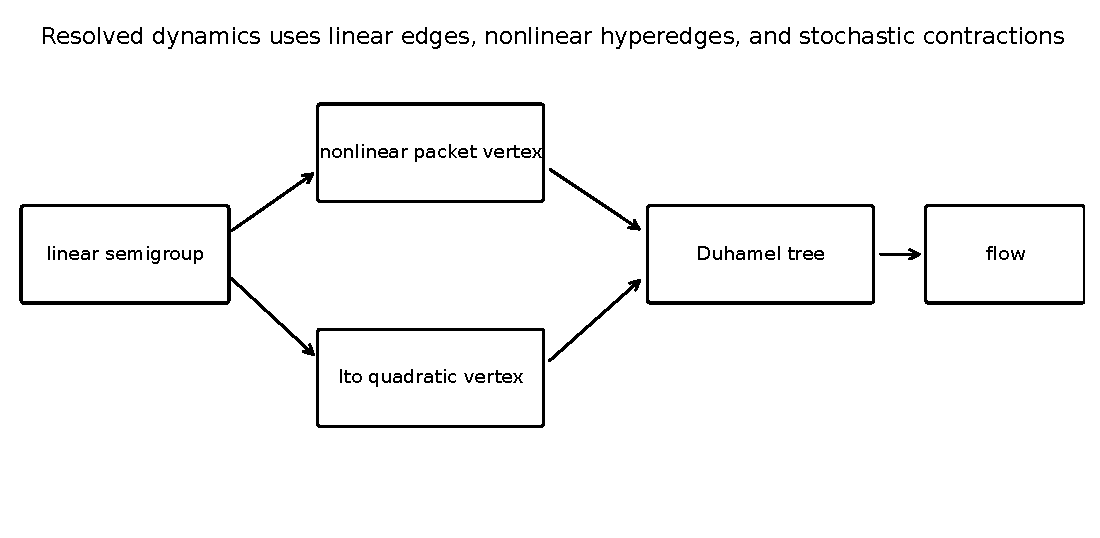
\includegraphics[width=.90\textwidth]{20_dynamics_stochastic.pdf}
\caption{Resolved dynamics combines semigroup edges, nonlinear vertices, and second order stochastic contractions inside one interaction tree.}
\label{fig:dynamics_stochastic}
\end{figure}

\section{Finite Resolution Logic}\label{sec:logic}

A calculation may be exact in one resolution and undecided in another. Resolution Logic records a Boolean predicate together with the resolution in which it is visible and, separately, a quantitative certificate for approximation error. The categorical language is indexed over the finite refinement poset.

Let \(r\preceq s\) mean that \(s\) refines \(r\). Let \(B_r\) be the Boolean algebra of predicates visible at resolution \(r\). Refinement gives a pullback
\[
 \rho_{sr}:B_r\longrightarrow B_s.
\]

\begin{definition}[Existential and universal refinement maps]\label{def:logic_adjoints}
For \(b\in B_s\), define \(\exists_{sr}b\) as the least coarse predicate whose pullback contains \(b\), and define \(\forall_{sr}b\) as the greatest coarse predicate whose pullback is contained in \(b\), whenever these extrema exist.
\end{definition}

\begin{theorem}[Refinement Galois connections]\label{thm:logic_galois}
For finite Boolean fibers,
\[
 \boxed{
 \exists_{sr}b\le a
 \iff
 b\le\rho_{sr}(a),
 }
\]
and
\[
 \boxed{
 \rho_{sr}(a)\le b
 \iff
 a\le\forall_{sr}b.
 }
\]
\end{theorem}

\begin{proof}
The existential map is defined as the least coarse upper approximation, so the first equivalence is its universal property. The universal map is the greatest coarse lower approximation, giving the second. Finite Boolean algebras guarantee existence by finite joins and meets.
\end{proof}

\begin{theorem}[Atomic completeness at finite resolution]\label{thm:logic_completeness}
If \(B_r\) is the power set Boolean algebra of the finite atomic packet set at resolution \(r\), every predicate is a unique join of visible atoms. Consequently, finite Boolean reasoning at a fixed resolution is complete.
\end{theorem}

\begin{proof}
Every subset is the union of its singleton atoms. Uniqueness is extensional equality of subsets.
\end{proof}

\begin{theorem}[Finite Beck Chevalley identity]\label{thm:beck_chevalley}
Consider a pullback square of finite packet maps
\[
 \begin{array}{ccc}
 r'&\longrightarrow&s'\\
 \downarrow&&\downarrow\\
 r&\longrightarrow&s.
 \end{array}
\]
For the induced power set Boolean fibers, pullback commutes with existential quantification around the square.
\end{theorem}

\begin{proof}
Both composites send a subset to the set of points whose image lies in it. Since the square is a pullback, the two conditions define the same subset.
\end{proof}

\begin{definition}[Certified approximation]\label{def:certified_approximation}
Write
\[
 \widehat x\Vdash_r x[\varepsilon]
\]
when \(\widehat x\) is represented at resolution \(r\) and
\[
 \norm{x-\widehat x}\le\varepsilon.
\]
\end{definition}

\begin{theorem}[Linear and multilinear transport]\label{thm:error_transport}
If \(\widehat x\Vdash_r x[\varepsilon]\) and \(A\) is bounded, then
\[
 A\widehat x\Vdash_s Ax[\norm{A}\varepsilon]
\]
for every declared source and target resolution of \(A\).

If \(B:X\times Y\to Z\) is bounded bilinear and
\[
 \widehat x\Vdash_r x[\varepsilon],
 \qquad
 \widehat y\Vdash_t y[\eta],
\]
then
\[
 B(\widehat x,\widehat y)
 \Vdash_u
 B(x,y)
 \left[
 \norm{B}
 \left(
 \norm{\widehat x}\eta
 +
 \norm{\widehat y}\varepsilon
 +
 \varepsilon\eta
 \right)
 \right].
\]
\end{theorem}

\begin{proof}
The linear rule is the operator norm bound. For the bilinear rule, write \(x=\widehat x+e\) and \(y=\widehat y+f\). Expand
\[
 B(x,y)-B(\widehat x,\widehat y)
 =
 B(e,\widehat y)
 +B(\widehat x,f)
 +B(e,f)
\]
and apply the bilinear norm bound.
\end{proof}

\begin{theorem}[Finite indexed semantics]\label{thm:indexed_semantics}
A finite resolution poset together with its Boolean predicate fibers, quantitative certificate fibers, pullback maps, adjoints, and sound transport rules forms a finite indexed semantics. Refinement acts functorially, and every declared inference preserves truth and its quantitative bound.
\end{theorem}

\begin{proof}
Functoriality of refinement follows from composition of packet maps. The Boolean rules are sound by \cref{thm:logic_galois,thm:logic_completeness,thm:beck_chevalley}. Quantitative transport is sound by \cref{thm:error_transport} and its multilinear iteration. The two fibers are kept distinct, so a valid Boolean implication does not erase its numerical certificate.
\end{proof}

\begin{figure}[t]
\centering
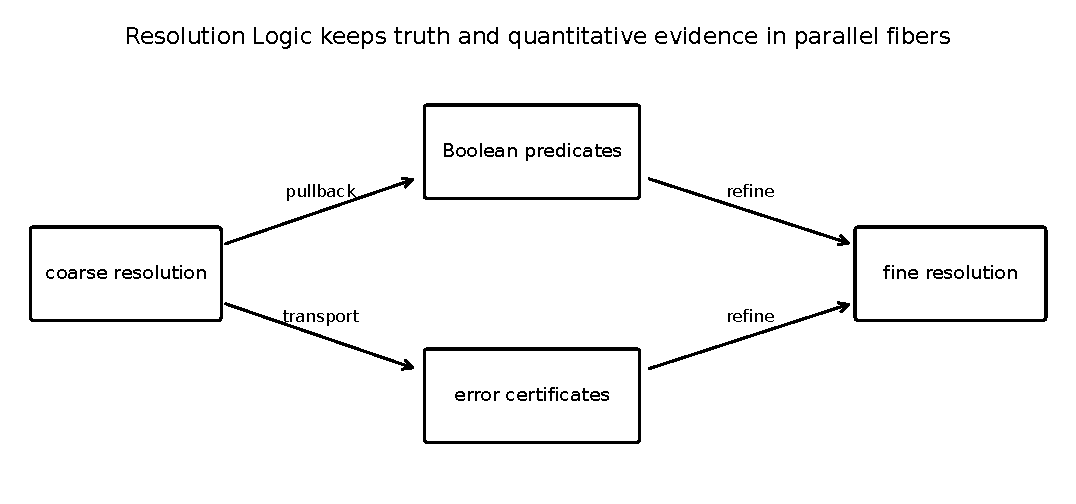
\includegraphics[width=.92\textwidth]{10_resolution_logic.pdf}
\caption{Resolution Logic carries predicates and quantitative certificates in parallel indexed fibers.}
\label{fig:resolution_logic}
\end{figure}

\subsection{Countable atomic Resolution Logic}

Let \(r:J\to I\) be a map from a countable fine packet set to a countable coarse packet set. Boolean predicates are subsets. Quantitative certificates take values in the complete lattice \([0,\infty]\).

\begin{theorem}[Countable atomic Boolean doctrine]\label{thm:countable_boolean_doctrine}
The inverse image map
\[
 r^*:\Pcal(I)\to\Pcal(J)
\]
has adjoints
\[
 \exists_r(B)
 =
 \{i:r^{-1}(i)\cap B\ne\varnothing\},
\]
\[
 \forall_r(B)
 =
 \{i:r^{-1}(i)\subseteq B\}.
\]
They satisfy the Galois connections
\[
 \exists_rB\subseteq A
 \Longleftrightarrow
 B\subseteq r^*A,
\]
\[
 r^*A\subseteq B
 \Longleftrightarrow
 A\subseteq\forall_rB.
\]
Arbitrary joins and meets exist, and the Beck Chevalley identity holds for pullback squares of countable packet sets.
\end{theorem}

\begin{proof}
All statements are set theoretic fiber calculations. Inverse image preserves arbitrary unions and intersections. The two adjunctions follow directly from the definitions. In a pullback square, both routes quantify over the same set theoretic fiber.
\end{proof}

\begin{theorem}[Complete quantitative fiber adjoints]\label{thm:quantitative_fiber_adjoints}
For a certificate \(c:J\to[0,\infty]\), define
\[
 (\exists_rc)(i)
 =
 \sup_{j:r(j)=i}c(j),
\]
\[
 (\forall_rc)(i)
 =
 \inf_{j:r(j)=i}c(j),
\]
with \(\sup\varnothing=0\) and \(\inf\varnothing=\infty\). Then \(\exists_r\dashv r^*\dashv\forall_r\) in the pointwise order. These operations preserve arbitrary joins or meets in the direction forced by the adjunctions.
\end{theorem}

\begin{proof}
For example,
\[
 \exists_rc\leq d
\]
means that every value of \(c\) in the fiber over \(i\) is bounded by \(d(i)\), which is equivalent to \(c\leq r^*d\). The right adjunction is dual.
\end{proof}

\begin{theorem}[Countable packet error transport]\label{thm:countable_error_transport}
Let \(T=(T_{ai})\) be a countable block transfer. Suppose input packets satisfy
\[
 \norm{x_i-\widehat x_i}\leq\varepsilon_i.
\]
Then the output packet error is bounded by
\[
 \boxed{
 \delta_a
 \leq
 \sum_i\norm{T_{ai}}\varepsilon_i.
 }
\]
If the scalar block norm matrix \(B_{ai}=\norm{T_{ai}}\) acts boundedly from \(\ell^2(I)\) to \(\ell^2(A)\), then
\[
 \boxed{
 \norm\delta_{\ell^2}
 \leq
 \norm B_{\ell^2\to\ell^2}
 \norm\varepsilon_{\ell^2}.
 }
\]
\end{theorem}

\begin{proof}
Apply the triangle inequality in every output packet and then the scalar operator bound.
\end{proof}

\begin{figure}[t]
\centering
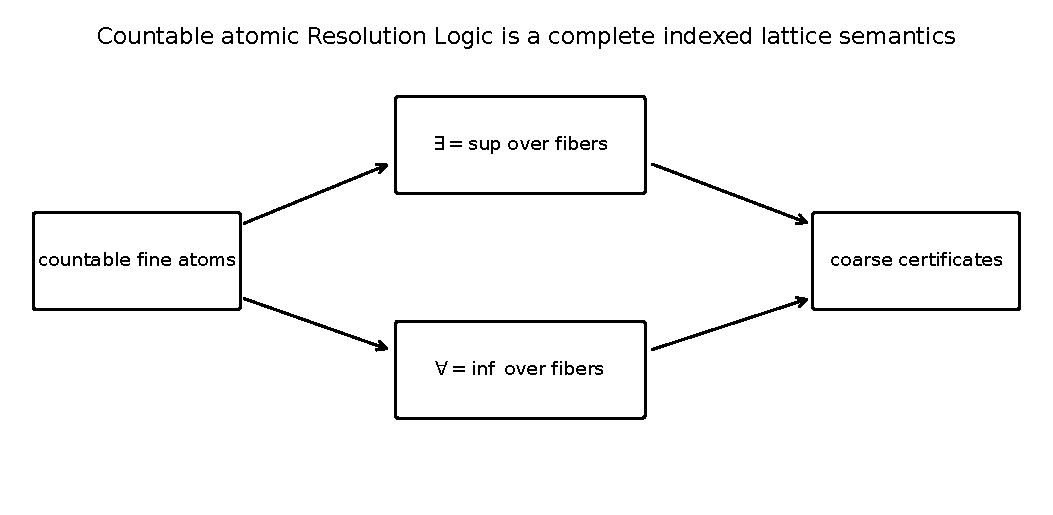
\includegraphics[width=.87\textwidth]{21_countable_logic.pdf}
\caption{Countable atomic predicates and complete lattice certificates admit exact refinement adjoints.}
\label{fig:countable_logic}
\end{figure}

\section{Concrete realizations and changes of resolution}\label{sec:realizations}

The preceding theory is abstract enough to preserve a chosen packet hierarchy, but concrete enough to recover familiar decompositions exactly. This section records several realizations. The point is not that Fourier analysis, wavelets, quantum measurements, or arithmetic residue classes become identical. The point is that each carries the same resolved data of packets, corners, refinement, reconstruction, and residual.

\subsection{Finite Fourier resolution}

Let \(G\) be a finite abelian group and let \(\widehat G\) be its character group. On \(\ell^2(G)\), define
\[
 P_\chi f
 =
 \widehat f(\chi)\chi,
 \qquad
 \widehat f(\chi)
 =
 \frac1{|G|}\sum_{g\in G}f(g)\overline{\chi(g)}.
\]

\begin{theorem}[Fourier realization]\label{thm:fourier_realization}
The family \((P_\chi)_{\chi\in\widehat G}\) is a complete orthogonal resolution. Fourier reconstruction and Parseval are the packet reconstruction and packet energy identities
\[
 \boxed{
 f=\sum_{\chi\in\widehat G}P_\chi f,
 }
\]
and
\[
 \boxed{
 \norm{f}_2^2
 =
 \sum_{\chi\in\widehat G}\norm{P_\chi f}_2^2.
 }
\]
Every convolution operator is diagonal in this resolution.
\end{theorem}

\begin{proof}
Character orthogonality gives
\[
 P_\chi P_\eta
 =
 \delta_{\chi\eta}P_\chi
\]
and completeness of the character basis gives the reconstruction. Orthogonality gives Parseval. If \(C_hf=h*f\), then
\[
 P_\chi C_hf
 =
 \widehat h(\chi)P_\chi f,
\]
so each packet is invariant and the transfer field is diagonal.
\end{proof}

\begin{remark}\label{rem:fourier_chart}
The group coordinate packets and the character packets are two resolutions of the same group algebra. The Fourier transform is a change of resolution. Resolution Theory does not declare one chart intrinsically superior. It records which transfer becomes sparse or diagonal in each chart.
\end{remark}

\subsection{Wavelet and polyphase resolution}

Let
\[
 V_0\subset V_1\subset\cdots\subset V_J
\]
be a finite multiresolution chain with
\[
 V_{j+1}=V_j\oplus W_j.
\]
Let \(P_j\) and \(D_j\) be the orthogonal projectors onto \(V_j\) and \(W_j\). Classical wavelet analysis supplies such systems under its usual hypotheses \Rcite{R16}. Polyphase and perfect reconstruction filter banks organize the same refinements through channel decompositions \Rcite{R17}.

\begin{theorem}[Multiresolution realization]\label{thm:wavelet_realization}
A finite orthogonal multiresolution analysis is a resolved Hilbert system in which
\[
 P_{j+1}=P_j+D_j
\]
is the refinement equation. For every \(f\in V_J\),
\[
 \boxed{
 f=P_0f+\sum_{j=0}^{J-1}D_jf
 }
\]
and
\[
 \boxed{
 \norm f^2
 =
 \norm{P_0f}^2
 +
 \sum_{j=0}^{J-1}\norm{D_jf}^2.
 }
\]
Every perfect reconstruction filter bank is a finite transfer system whose analysis and synthesis maps compose to the identity.
\end{theorem}

\begin{proof}
The refinement equation gives a telescoping orthogonal sum. Reconstruction and energy follow from repeated use of the Pythagorean theorem. A perfect reconstruction filter bank is precisely a pair of resolved transfers \(A\) and \(S\) with \(SA=I\). Its channel operators are the packet corners of \(A\) and \(S\).
\end{proof}

\begin{figure}[t]
\centering
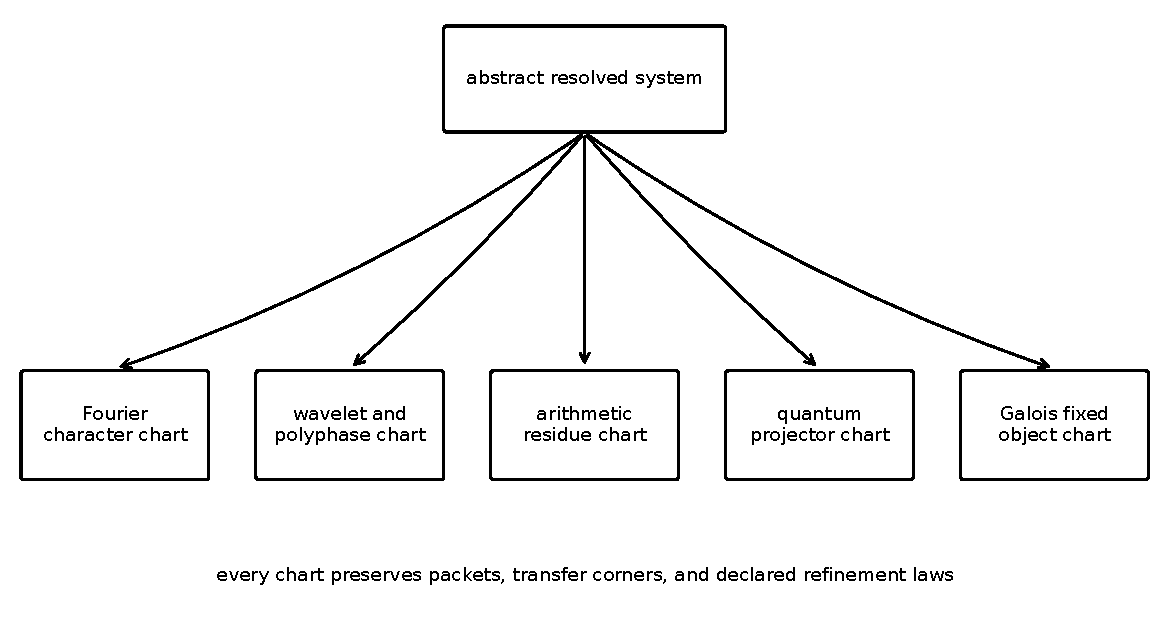
\includegraphics[width=.91\textwidth]{11_realization_atlas.pdf}
\caption{Fourier, wavelet, quantum, and arithmetic systems are concrete resolved charts with different native packet geometries.}
\label{fig:realization_atlas}
\end{figure}

\subsection{Quantum projector charts}

A finite projective measurement on a Hilbert space is a complete orthogonal projector family. A quantum channel is a linear transfer on operators and can be resolved by input and output measurement projectors. Standard quantum information supplies the ambient operator theory \Rcite{R19}.

\begin{proposition}[Quantum measurement realization]\label{prop:quantum_realization}
Let \((P_i)_i\) and \((Q_a)_a\) be projective measurements. Every operator \(T\) has the exact transition decomposition
\[
 \boxed{
 T=\sum_{a,i}Q_aTP_i.
 }
\]
Two projective measurements admit one common orthogonal refinement exactly when every \(P_i\) commutes with every \(Q_a\). Otherwise their exact relation is the projector atlas of mixed corners \(Q_aTP_i\).
\end{proposition}

\begin{proof}
The decomposition is \cref{thm:mixed_blocks}. The refinement assertion is \cref{thm:common_refinement}.
\end{proof}

\subsection{Arithmetic residue resolution}

Let \(a:\NN\to\CC\) be an arithmetic sequence. For a positive integer \(q\), define
\[
 a_{q,r}(m)=a(qm+r),
 \qquad
 0\le r<q.
\]
If
\[
 A(z)=\sum_{n\ge0}a(n)z^n,
\]
put
\[
 A_{q,r}(u)=\sum_{m\ge0}a(qm+r)u^m.
\]

\begin{theorem}[Arithmetic polyphase realization]\label{thm:arithmetic_polyphase}
The arithmetic sequence has the exact packet reconstruction
\[
 \boxed{
 A(z)
 =
 \sum_{r=0}^{q-1}z^rA_{q,r}(z^q).
 }
\]
If \(Q=mq\), then the refinement law is
\[
 \boxed{
 A_{q,r}(u)
 =
 \sum_{b=0}^{m-1}
 u^bA_{Q,r+qb}(u^m).
 }
\]
Thus residue classes form a resolved system and divisibility of moduli is its refinement order.
\end{theorem}

\begin{proof}
Write every integer uniquely as \(qn+r\). For the refinement, write the packet index uniquely as \(mn+b\).
\end{proof}

\begin{corollary}[Prime packet realization]\label{cor:prime_packet_realization}
Taking \(a(n)=\Lambda(n)\) or \(a(n)=\mathbf 1_{\mathbb P}(n)\) gives an arithmetic realization of Resolution Theory. Refining a squarefree modulus by a new prime separates deterministic divisibility packets from the residual distribution among surviving packets. On the surviving unit packets, additive child modes and multiplicative character modes are connected by the finite Gauss change of resolution in \cref{thm:gauss_resolution_change}.
\end{corollary}

\begin{proof}
The first statement is \cref{thm:arithmetic_polyphase}. The deterministic forbidden packets are the residues divisible by the newly introduced prime. Fourier and character coordinates are bases of the corresponding finite function space.
\end{proof}

\subsection{Sieve packets and the additive to multiplicative chart change}

Let
\[
 M_{q,a}(x)
 =
 \frac qx
 \sum_{\substack{n\leq x\\n\equiv a\bmod q}}
 \Lambda(n).
\]
Let \(p\nmid q\) be prime and let \((a,q)=1\). The child packet values are
\[
 F_b=M_{pq,a+qb}(x),
 \qquad
 0\leq b<p.
\]
Exactly one child
\[
 b_0\equiv-aq^{-1}\pmod p
\]
is divisible by \(p\).

\begin{theorem}[Arithmetic sieve line decomposition]\label{thm:arithmetic_sieve_line}
Let
\[
 M=\frac1p\sum_bF_b,
 \qquad
 K=F_{b_0},
 \qquad
 C=\frac{pM-K}{p-1}.
\]
Then the centered child vector has the orthogonal decomposition
\[
 \boxed{
 (F_b-M)_b
 =
 (K-M)s_{b_0}+E,
 }
\]
where
\[
 s_{b_0}
 =
 e_{b_0}
 -
 \frac1{p-1}\sum_{b\ne b_0}e_b,
\]
and
\[
 E_{b_0}=0,
 \qquad
 \sum_{b\ne b_0}E_b=0.
\]
Consequently,
\[
 \boxed{
 \frac1p\sum_b\abs{F_b-M}^2
 =
 \frac{\abs{K-M}^2}{p-1}
 +
 \frac1p\sum_{b\ne b_0}\abs{F_b-C}^2.
 }
\]
The first term is the deterministic sieve direction and the second is the survivor residual.
\end{theorem}

\begin{proof}
The vector \(s_{b_0}\) lies in the zero sum detail space. The survivor residual is supported away from \(b_0\) and has zero survivor sum, so it is orthogonal to \(s_{b_0}\). Direct projection gives the coefficient \(K-M\), and Pythagoras gives the energy identity.
\end{proof}

Let \(E_a(c)\) be the survivor residual in Chinese remainder coordinates \(c\in\FF_p^\times\), extended by \(E_a(0)=0\). Define the additive modes
\[
 A_a(k)
 =
 \frac1p\sum_{c\in\FF_p}E_a(c)e^{-2\pi ikc/p}
\]
and the multiplicative modes
\[
 B_a(\eta)
 =
 \frac1{p-1}
 \sum_{c\in\FF_p^\times}
 E_a(c)\overline{\eta(c)}.
\]

\begin{theorem}[Finite Gauss change of resolution]\label{thm:gauss_resolution_change}
For every nonzero additive frequency \(k\),
\[
 \boxed{
 A_a(k)
 =
 \frac1p
 \sum_{\eta\ne\eta_0}
 \tau(\eta)\overline{\eta(-k)}B_a(\eta),
 }
\]
where
\[
 \tau(\eta)
 =
 \sum_{c\in\FF_p^\times}\eta(c)e^{2\pi ic/p}.
\]
Moreover,
\[
 \boxed{
 \sum_{k=1}^{p-1}\abs{A_a(k)}^2
 =
 \frac{p-1}{p}
 \sum_{\eta\ne\eta_0}\abs{B_a(\eta)}^2.
 }
\]
Thus additive child wavelets and nonprincipal local Dirichlet characters are two exact charts of the same survivor residual.
\end{theorem}

\begin{proof}
Multiplicative Fourier inversion gives
\[
 E_a(c)=\sum_{\eta\ne\eta_0}B_a(\eta)\eta(c).
\]
Insert this into the additive transform and identify the inner sum as the Gauss sum. Additive and multiplicative Parseval give the energy identity.
\end{proof}

\begin{figure}[t]
\centering
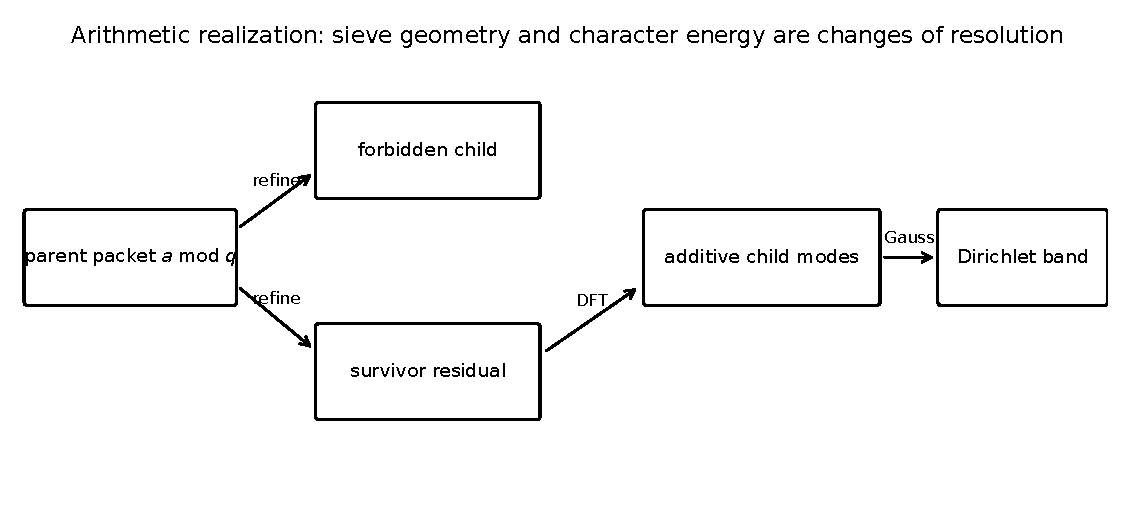
\includegraphics[width=.95\textwidth]{22_prime_packet_gauss.pdf}
\caption{The arithmetic realization separates deterministic divisibility from survivor imbalance, then changes from additive packet modes to multiplicative character modes.}
\label{fig:prime_packet_gauss}
\end{figure}

\begin{remark}\label{rem:arithmetic_scope}
The arithmetic realization does not itself prove a new prime number theorem. It identifies the native packet system in which sieve support, character energy, conductor refinement, and Mellin scale can be studied inside the general resolved calculus.
\end{remark}

\subsection{A realization dictionary}

\begin{theorem}[Resolved realization dictionary]\label{thm:realization_dictionary}
The systems in \cref{thm:fourier_realization,thm:wavelet_realization,prop:quantum_realization,thm:arithmetic_polyphase} are concrete realizations of the same finite resolved axioms. In each case:
\begin{enumerate}
\item a packet is the range of a named idempotent or coordinate selector
\item a transfer block is a mixed corner between source and target packets
\item refinement is an orthogonal or coordinate decomposition of one packet into descendants
\item reconstruction is the sum of all packet components
\item a change of chart is an invertible transfer between two resolved coordinate systems
\item compression retains selected blocks and names the omitted residual.
\end{enumerate}
\end{theorem}

\begin{proof}
For Fourier and quantum systems the packets are orthogonal projectors. For wavelets they are scale and detail projectors. For arithmetic residue packets they are coordinate idempotents in the finite residue function algebra. The remaining items follow from the reconstruction and refinement formulas already proved.
\end{proof}


\section{Galois symmetry as a resolved realization}\label{sec:galois_realization}

Galois theory organizes intermediate objects through symmetries and fixed points. Resolution Theory enlarges that pattern from fields and invertible group actions to projector systems, conditional expectations, noncommuting charts, residuals, nonlinear transfers, and approximate invariance. The finite semisimple Galois correspondence embeds directly into the resolved projector calculus.

\subsection{Fixed point projectors and the subgroup lattice}

\begin{definition}[Semisimple Galois resolution datum]\label{def:galois_resolution_datum}
A semisimple Galois resolution datum is a finite group \(G\), a finite dimensional Hilbert space \(V\), and a unitary representation
\[
 U:G\longrightarrow\mathcal U(V).
\]
For a subgroup \(H\leq G\), define the fixed point averaging operator
\[
 \boxed{
 P_H
 =
 \frac1{|H|}\sum_{h\in H}U_h.
 }
\]
\end{definition}

\begin{theorem}[Reynolds fixed point projector]\label{thm:reynolds_projector}
For every subgroup \(H\leq G\), the operator \(P_H\) is the orthogonal projector onto
\[
 V^H
 =
 \{v\in V:U_hv=v\text{ for every }h\in H\}.
\]
If \(H\leq J\), then
\[
 \boxed{
 P_HP_J=P_JP_H=P_J.
 }
\]
Thus subgroup inclusion reverses the projector order.
\end{theorem}

\begin{proof}
Self adjointness follows from invariance of \(H\) under inversion. For idempotence,
\[
 P_H^2
 =
 \frac1{|H|^2}\sum_{h,k\in H}U_{hk}
 =
 \frac1{|H|}\sum_{g\in H}U_g
 =P_H.
\]
Every \(H\) fixed vector is unchanged by \(P_H\). Conversely, if \(P_Hv=v\), then for \(a\in H\),
\[
 U_aP_Hv
 =
 \frac1{|H|}\sum_{h\in H}U_{ah}v
 =P_Hv=v.
\]
Hence the range is \(V^H\). If \(H\leq J\), then \(V^J\subseteq V^H\). Orthogonal projections onto nested subspaces commute and multiply to the smaller range projector.
\end{proof}

\begin{theorem}[Resolution form of the fundamental Galois correspondence]\label{thm:resolution_galois_correspondence}
Let \(L/K\) be a finite Galois extension, let \(G=\Gal(L/K)\), and fix an embedding \(\iota:K\hookrightarrow\CC\). After extending scalars along \(\iota\) and averaging the inner product over \(G\), the assignment
\[
 \boxed{
 H\longmapsto P_H
 }
\]
is an injective order reversing map from the subgroup lattice of \(G\) to the projection lattice of the Galois module. Its range satisfies
\[
 \boxed{
 \ran P_H
 =
 L^H\otimes_K\CC.
 }
\]
For an intermediate field \(E\),
\[
 \boxed{
 H\leq\Gal(L/E)
 \quad\Longleftrightarrow\quad
 E\subseteq L^H.
 }
\]
The two closure operations are identities, so the subgroup and fixed field lattices are in an order reversing isomorphism.
\end{theorem}

\begin{proof}
Averaging makes the Galois action unitary. The chosen embedding extends to the finite separable algebra after passage to an algebraic closure, and invariants commute with scalar extension because the averaging idempotent exists in characteristic zero. Hence \(P_H\) has the stated range by \cref{thm:reynolds_projector}. The displayed equivalence follows directly from the definitions. The finite Galois correspondence gives
\[
 \Gal(L/L^H)=H,
 \qquad
 L^{\Gal(L/E)}=E
\]
\Rcite{R28}. Therefore distinct subgroups have distinct fixed ranges and the assignment is injective.
\end{proof}

\begin{figure}[t]
\centering
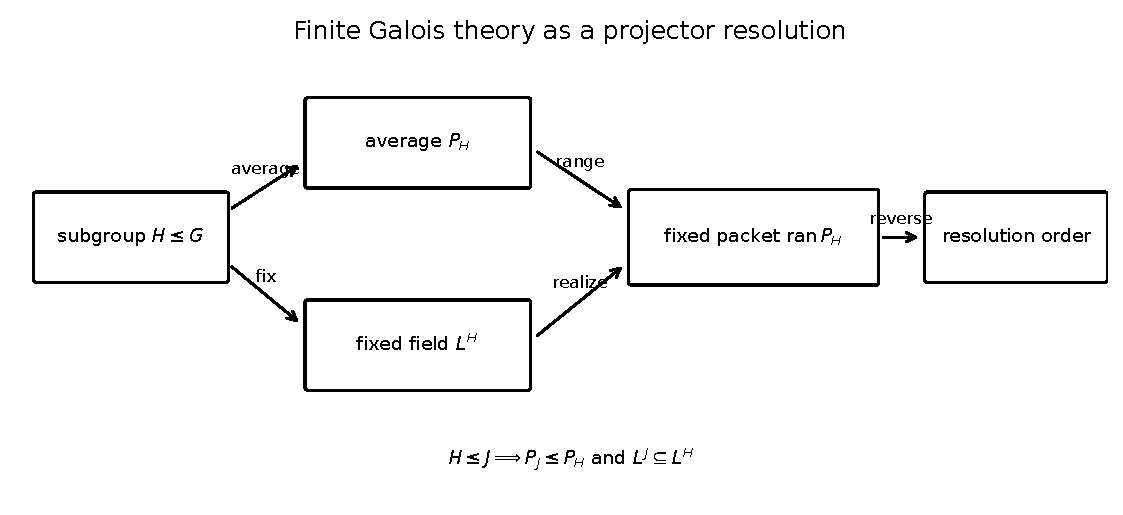
\includegraphics[width=.95\textwidth]{23_galois_resolution_dictionary.pdf}
\caption{Finite Galois theory embeds into Resolution Theory by sending a subgroup to its fixed point projector and fixed object. The order is reversed.}
\label{fig:galois_dictionary}
\end{figure}

\begin{theorem}[Lattice operations and compatible fixed resolutions]\label{thm:galois_lattice_operations}
In the faithful field or regular realization of \cref{thm:resolution_galois_correspondence}, let \(H,J\leq G\). Then
\[
 \boxed{
 L^{\langle H,J\rangle}
 =
 L^H\cap L^J,
 }
\]
\[
 \boxed{
 L^{H\cap J}
 =
 L^HL^J.
 }
\]
The orthogonal projector onto \(V^H\cap V^J\) is \(P_{\langle H,J\rangle}\). Moreover, the following are equivalent:
\begin{enumerate}
\item \(HJ=JH\)
\item \(HJ\) is a subgroup
\item \(P_H\) and \(P_J\) commute.
\end{enumerate}
When these conditions hold,
\[
 \boxed{
 P_HP_J=P_JP_H=P_{HJ}.
 }
\]
\end{theorem}

\begin{proof}
The fixed field identities are the meet and join formulas in the finite Galois correspondence. A vector is fixed by both \(H\) and \(J\) exactly when it is fixed by the subgroup they generate. If \(HJ=JH\), then each element of \(HJ\) has \(|H\cap J|\) representations as a product \(hj\), so
\[
 P_HP_J
 =
 \frac1{|H||J|}\sum_{h,j}U_{hj}
 =
 \frac1{|HJ|}\sum_{g\in HJ}U_g
 =P_{HJ}.
\]
The same formula holds in the reverse order. Conversely, in the regular representation the support of \(P_HP_J\) is \(HJ\) and the support of \(P_JP_H\) is \(JH\). Equality therefore forces \(HJ=JH\). Faithful Galois realization reduces to that case through a normal basis.
\end{proof}

\begin{corollary}[Common refinement and the Galois atlas boundary]\label{cor:galois_common_refinement}
Permutable subgroups give commuting fixed resolutions and therefore admit the exact common refinement supplied by \cref{thm:common_refinement}. Nonpermutable subgroups still have the exact common fixed packet \(P_{\langle H,J\rangle}\), but the products \(P_HP_J\) and \(P_JP_H\) are not projectors in general. They must be retained as mixed atlas corners.
\end{corollary}

\begin{proof}
Apply \cref{thm:galois_lattice_operations,thm:common_refinement}. The noncommuting conclusion is the defining boundary of a projector atlas.
\end{proof}

\begin{theorem}[Normality, centrality, and quotient compression]\label{thm:normality_centrality}
In the faithful field or regular realization, let \(H\leq G\). The following are equivalent:
\begin{enumerate}
\item \(H\triangleleft G\)
\item the group algebra average
\[
 e_H=\frac1{|H|}\sum_{h\in H}h
\]
is central in \(\CC[G]\)
\item \(P_HU_g=U_gP_H\) for every \(g\in G\)
\item the fixed range \(V^H\) is \(G\) invariant
\item the fixed field \(L^H\) is Galois over \(K\).
\end{enumerate}
When these conditions hold, the compressed action on \(V^H\) factors canonically through \(G/H\), and
\[
 \boxed{
 \Gal(L^H/K)\cong G/H.
 }
\]
\end{theorem}

\begin{proof}
Conjugation sends \(e_H\) to \(e_{gHg^{-1}}\). Hence centrality is equivalent to normality. The represented operator satisfies
\[
 U_gP_HU_g^{-1}=P_{gHg^{-1}},
\]
so commutation and invariance are equivalent to the same condition. The field statement and quotient identification are the normal subgroup part of the fundamental Galois correspondence.
\end{proof}

\begin{figure}[t]
\centering
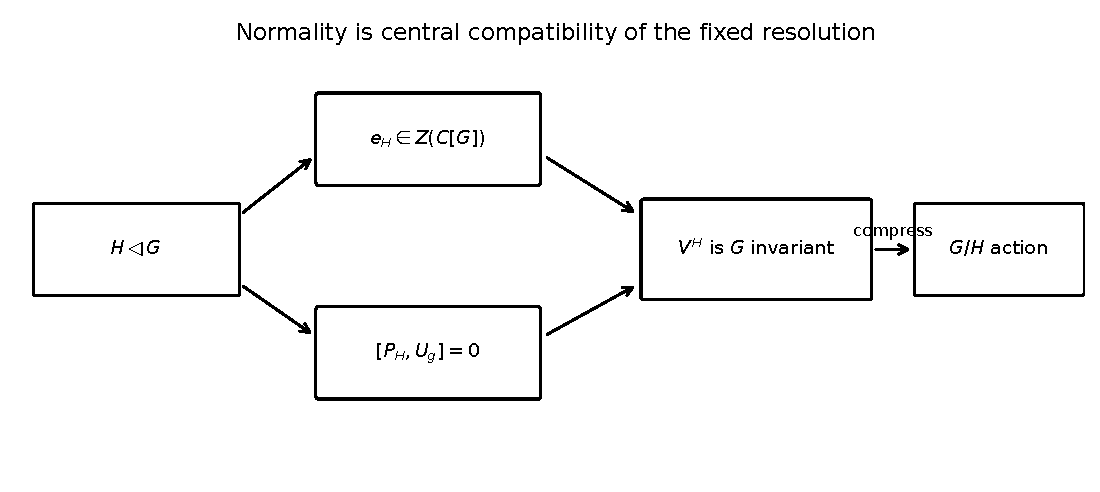
\includegraphics[width=.92\textwidth]{24_normality_quotient.pdf}
\caption{Normality is central compatibility of the fixed projector. The compressed action then descends to the quotient group.}
\label{fig:normality_quotient}
\end{figure}

\subsection{Noncommutative fixed point resolutions}

\begin{theorem}[Finite group conditional expectation]\label{thm:fixed_point_expectation}
Let a finite group \(G\) act on a unital \(C^*\) algebra \(A\) by star automorphisms \(\alpha_g\). For \(H\leq G\), define
\[
 \boxed{
 E_H(a)
 =
 \frac1{|H|}\sum_{h\in H}\alpha_h(a).
 }
\]
Then \(E_H\) is a faithful unital completely positive conditional expectation onto
\[
 A^H=\{a:\alpha_h(a)=a\text{ for every }h\in H\}.
\]
If \(H\leq J\), then
\[
 E_HE_J=E_JE_H=E_J.
\]
If \(H\triangleleft G\), then \(E_H\) commutes with the full action and \(G/H\) acts on \(A^H\).
\end{theorem}

\begin{proof}
An average of star automorphisms is unital and completely positive. The group averaging calculation gives idempotence and shows that the range is \(A^H\). If \(a\geq0\) and \(E_H(a)=0\), then the sum of positive elements \(\alpha_h(a)\) is zero, so every term is zero and hence \(a=0\). This proves faithfulness. The subgroup and normality statements follow from the same averaging and conjugation identities used in \cref{thm:reynolds_projector,thm:normality_centrality}.
\end{proof}

\begin{corollary}[GNS projector implementation]\label{cor:expectation_gns_projector}
Let \(\varphi\) be a \(G\) invariant state on \(A\), and let \((\pi_\varphi,\Hh_\varphi,\Omega_\varphi)\) be its GNS representation. Then \(E_H\) is implemented on \(\Hh_\varphi\) by the orthogonal projector onto the \(H\) fixed subspace. Thus fixed point algebras are noncommutative Galois resolutions inside the universal projector corner theory.
\end{corollary}

\begin{proof}
The invariant state makes the automorphisms unitary in the GNS representation. The average of those unitaries is the projector of \cref{thm:reynolds_projector}, and it sends \(\pi_\varphi(a)\Omega_\varphi\) to \(\pi_\varphi(E_Ha)\Omega_\varphi\).
\end{proof}

\subsection{Trace, norm, and Fourier Galois charts}

\begin{proposition}[Trace and norm as packet transfers]\label{prop:galois_trace_norm}
Let \(L/K\) be finite Galois with group \(G\), and let \(H\leq G\). Then
\[
 \boxed{
 \Tr_{L/L^H}(x)
 =
 \sum_{h\in H}h(x)
 =
 |H|P_Hx.
 }
\]
The norm is the nonlinear packet transfer
\[
 \boxed{
 N_{L/L^H}(x)
 =
 \prod_{h\in H}h(x).
 }
\]
For a subgroup chain \(H\leq J\leq G\), trace and norm satisfy the exact coarsening laws
\[
 \Tr_{L/L^J}
 =
 \Tr_{L^H/L^J}\circ\Tr_{L/L^H},
\]
\[
 N_{L/L^J}
 =
 N_{L^H/L^J}\circ N_{L/L^H}.
\]
\end{proposition}

\begin{proof}
The trace and norm are the sum and product over the embeddings of \(L\) fixing \(L^H\), which are exactly the elements of \(H\). Transitivity follows by partitioning embeddings according to the field tower. The trace is linear packet aggregation. The norm is a homogeneous nonlinear transfer of degree \(|H|\).
\end{proof}

\begin{theorem}[Abelian Fourier Galois chart]\label{thm:abelian_fourier_galois}
Let \(G\) be finite abelian and let the coefficient field contain all character values. For \(\chi\in\widehat G\), define
\[
 e_\chi
 =
 \frac1{|G|}\sum_{g\in G}\overline{\chi(g)}U_g.
\]
Then the \(e_\chi\) are mutually orthogonal character projectors with sum \(I\). For \(H\leq G\), let
\[
 H^\perp
 =
 \{\chi\in\widehat G:\chi|_H=1\}.
\]
Then
\[
 \boxed{
 P_H
 =
 \sum_{\chi\in H^\perp}e_\chi.
 }
\]
For \(x\) in a Galois module, the classical Lagrange resolvent
\[
 \mathcal R_\chi(x)
 =
 \sum_{g\in G}\overline{\chi(g)}g(x)
\]
satisfies
\[
 \boxed{
 \mathcal R_\chi(x)=|G|e_\chi x.
 }
\]
Thus Galois resolvents are Fourier packet coordinates.
\end{theorem}

\begin{proof}
Character orthogonality gives the projector relations. Summing \(e_\chi\) over \(H^\perp\) produces
\[
 \frac1{|G|}\sum_{g\in G}
 \left(\sum_{\chi\in H^\perp}\overline{\chi(g)}\right)U_g.
\]
The inner sum is \(|G/H|\) when \(g\in H\) and zero otherwise. The result is \(P_H\). The resolvent identity is immediate from the definition.
\end{proof}

\begin{theorem}[Normal basis as a change of Galois resolution]\label{thm:normal_basis_resolution}
Let \(L/K\) be finite Galois with group \(G\). The normal basis theorem identifies the Galois module \(L\) with the regular module \(K[G]\) \Rcite{R28}. Under this identification:
\begin{enumerate}
\item group coordinate packets are the orbit basis \(\{g\alpha:g\in G\}\)
\item subgroup fixed projectors are group averages
\item in the abelian case, character packets are the Fourier transform of the group coordinate packets
\item trace, norm, and Lagrange resolvents become resolved transfers between these charts.
\end{enumerate}
\end{theorem}

\begin{proof}
Choose a normal element \(\alpha\) whose orbit is a \(K\) basis. The map \(K[G]\to L\) sending \(\sum c_gg\) to \(\sum c_gg(\alpha)\) is a \(K[G]\) module isomorphism. The remaining statements follow from \cref{thm:reynolds_projector,prop:galois_trace_norm,thm:abelian_fourier_galois}.
\end{proof}

\begin{figure}[t]
\centering
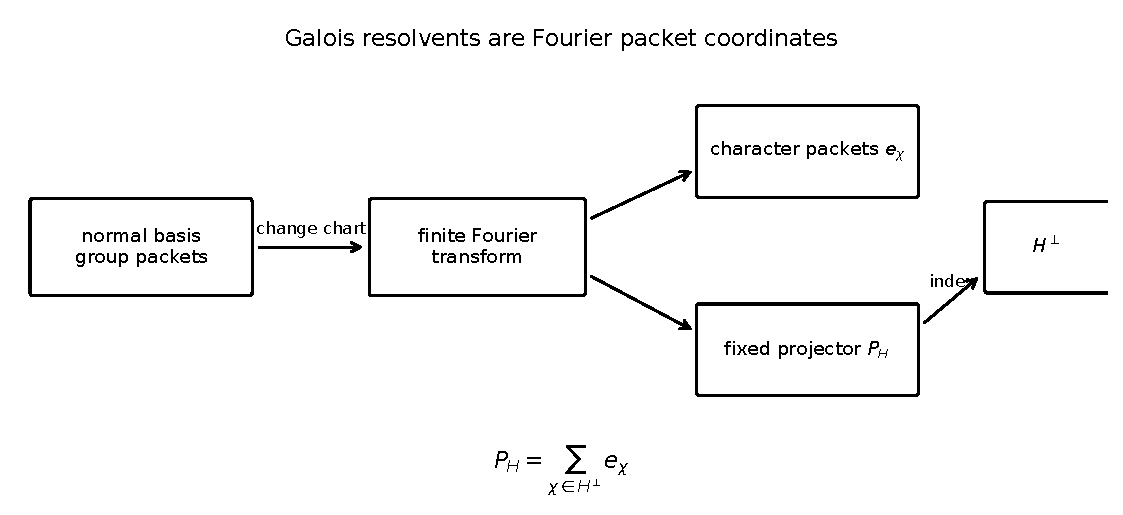
\includegraphics[width=.94\textwidth]{25_fourier_galois_chart.pdf}
\caption{A normal basis gives group coordinate packets. Character projectors give the Fourier Galois chart, and subgroup projectors are annihilator sums.}
\label{fig:fourier_galois_chart}
\end{figure}

\subsection{Galois closures as projector atlases}

\begin{theorem}[Conjugate field atlas]\label{thm:galois_closure_atlas}
Let \(M/K\) be finite separable, let \(L/K\) be a finite Galois closure with group \(G\), and put
\[
 H=\Gal(L/M).
\]
For \(g\in G\),
\[
 \boxed{
 g(M)=L^{gHg^{-1}},
 \qquad
 U_gP_HU_g^{-1}=P_{gHg^{-1}}.
 }
\]
The conjugate intermediate fields therefore form a projector atlas. The following are equivalent:
\begin{enumerate}
\item \(M/K\) is Galois
\item \(H\triangleleft G\)
\item every conjugate projector equals \(P_H\)
\item the atlas consists of one global fixed chart.
\end{enumerate}
\end{theorem}

\begin{proof}
The first identity is the conjugation rule for fixed fields. The second is the represented averaging identity. The equivalences are \cref{thm:normality_centrality}.
\end{proof}

\begin{theorem}[Core and normal closure projectors]\label{thm:core_normal_closure}
With the preceding notation, define
\[
 \Core_G(H)=\bigcap_{g\in G}gHg^{-1},
\]
\[
 \Ncl_G(H)=\left\langle gHg^{-1}:g\in G\right\rangle.
\]
Then
\[
 \boxed{
 L^{\Core_G(H)}
 =
 \prod_{g\in G}g(M),
 }
\]
is the smallest Galois extension of \(K\) inside \(L\) containing \(M\), while
\[
 \boxed{
 L^{\Ncl_G(H)}
 =
 \bigcap_{g\in G}g(M)
 }
\]
is the largest Galois subfield of \(M\) over \(K\). The associated projectors are the canonical global envelopes of the conjugate atlas.
\end{theorem}

\begin{proof}
Composita correspond to intersections of subgroups, while intersections of fields correspond to generated subgroups. The core is the largest normal subgroup contained in \(H\). Its fixed field is therefore the smallest Galois extension containing \(M\). The normal closure of \(H\) is the smallest normal subgroup containing \(H\). Its fixed field is the largest Galois field contained in \(M\).
\end{proof}

\begin{figure}[t]
\centering
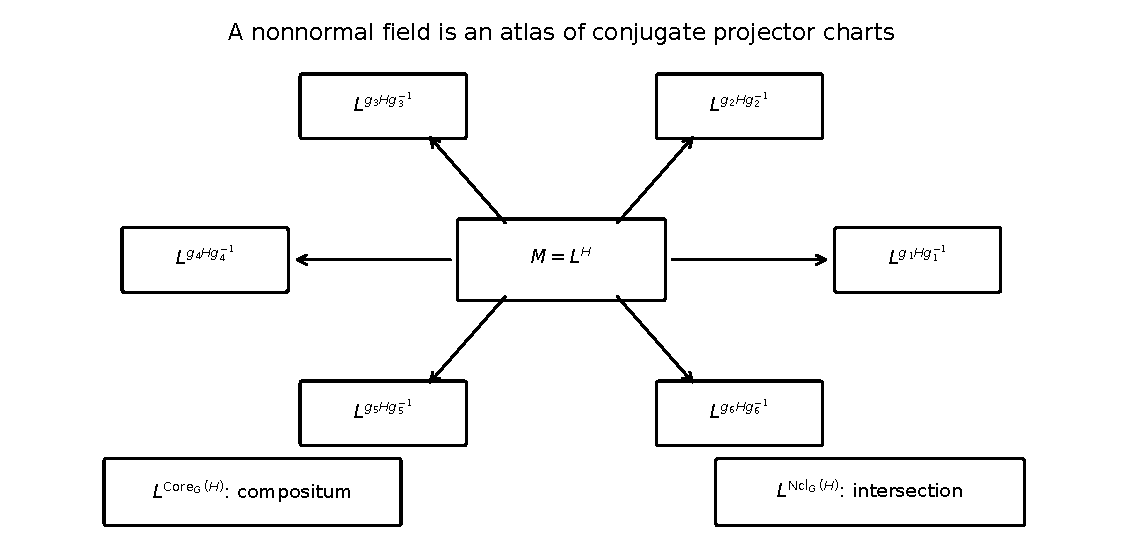
\includegraphics[width=.93\textwidth]{26_galois_closure_atlas.pdf}
\caption{A nonnormal intermediate field appears as an atlas of conjugate fixed projectors. The subgroup core and normal closure give the two canonical global envelopes.}
\label{fig:galois_closure_atlas}
\end{figure}

\subsection{Induction, restriction, and double coset transfer}

\begin{theorem}[Mackey packet decomposition]\label{thm:mackey_packet_decomposition}
Let \(H,K\leq G\), and let \(W\) be a finite dimensional representation of \(H\). Choose representatives \(x\) for \(K\backslash G/H\). Then
\[
 \boxed{
 \Res_K^G\Ind_H^GW
 \cong
 \bigoplus_{x\in K\backslash G/H}
 \Ind_{K\cap xHx^{-1}}^K
 \left({}^x\Res_{H\cap x^{-1}Kx}^HW\right).
 }
\]
Each double coset is one exact transfer packet between the \(H\) and \(K\) symmetry charts.
\end{theorem}

\begin{proof}
Decompose \(G\) as the disjoint union of double cosets \(KxH\). The induced module consists of functions on \(G\) with the usual \(H\) covariance. Functions supported on distinct double cosets form invariant direct summands under \(K\). Identifying one summand with functions on \(K\) having covariance under \(K\cap xHx^{-1}\) gives the displayed induced module. This is the finite Mackey decomposition \Rcite{R22}.
\end{proof}

\begin{corollary}[Double cosets as atlas transition packets]\label{cor:double_coset_atlas}
Restriction and induction do not require one common subgroup chart. The double coset decomposition supplies the exact mixed corners between two subgroup resolutions, in the same sense that noncommuting projector atlases are connected by mixed transfer blocks.
\end{corollary}

\begin{proof}
The summands in \cref{thm:mackey_packet_decomposition} are indexed by the transition orbits of the left \(K\) and right \(H\) actions. They are therefore the canonical packet transitions between the two symmetry charts.
\end{proof}

\section{Ramification as a resolution filtration}\label{sec:ramification_resolution}

Let \(L/K\) be a finite Galois extension of local fields with group \(G\). Let
\[
 G_{-1}=G,
 \qquad
 G_0=I,
 \qquad
 G_1\supseteq G_2\supseteq\cdots
\]
be the lower ramification filtration. Let \(V\) be a finite dimensional unitary complex representation of \(G\).

\begin{definition}[Ramification resolution]\label{def:ramification_resolution}
For \(i\geq0\), define
\[
 P_i
 =
 \frac1{|G_i|}\sum_{g\in G_i}U_g.
\]
Choose \(m\) with \(G_{m+1}=1\), and put
\[
 D_i=P_{i+1}-P_i,
 \qquad
 0\leq i\leq m.
\]
\end{definition}

\begin{theorem}[Orthogonal ramification details]\label{thm:ramification_details}
The projectors are nested:
\[
 P_0\leq P_1\leq\cdots\leq P_{m+1}=I.
\]
The detail projectors \(D_i\) are mutually orthogonal and
\[
 \boxed{
 V
 =
 V^{I}
 \mathbin\oplus
 \bigoplus_{i=0}^{m}D_iV.
 }
\]
Every \(P_i\) commutes with the decomposition group action, so each detail packet carries the quotient action permitted by the corresponding normal ramification subgroup.
\end{theorem}

\begin{proof}
The ramification groups are nested and normal. Apply \cref{thm:reynolds_projector,thm:normality_centrality}. Differences of nested orthogonal projections are orthogonal projections, and the telescoping sum gives the decomposition.
\end{proof}

\begin{theorem}[Artin conductor as weighted unresolved resolution]\label{thm:artin_conductor_resolution}
Let \(a(V)\) be the Artin conductor exponent and \(\operatorname{Sw}(V)\) the Swan conductor. Then
\[
 \boxed{
 a(V)
 =
 \sum_{i\geq0}
 \frac{|G_i|}{|G_0|}
 \Tr(I-P_i),
 }
\]
\[
 \boxed{
 \operatorname{Sw}(V)
 =
 \sum_{i\geq1}
 \frac{|G_i|}{|G_0|}
 \Tr(I-P_i).
 }
\]
If \(d_j=\operatorname{rank}D_j\), then
\[
 \boxed{
 a(V)
 =
 \sum_{j=0}^{m}
 d_j
 \sum_{i=0}^{j}
 \frac{|G_i|}{|G_0|}.
 }
\]
Thus the conductor is the weighted total rank of ramification details that remain unresolved at each scale.
\end{theorem}

\begin{proof}
The classical conductor formula is
\[
 a(V)
 =
 \sum_{i\geq0}
 \frac{|G_i|}{|G_0|}
 \operatorname{codim}V^{G_i}
\]
\Rcite{R23}. Since \(P_i\) is the projector onto \(V^{G_i}\), the codimension is \(\Tr(I-P_i)\). The Swan formula omits the tame term \(i=0\). Finally,
\[
 \operatorname{codim}V^{G_i}
 =
 \sum_{j\geq i}d_j,
\]
and reversing the finite sums gives the detail formula.
\end{proof}

\begin{proposition}[Upper numbering as a scale change]\label{prop:herbrand_scale_change}
The upper ramification filtration \(G^u\) gives the same nested fixed projectors as the lower filtration, with the scale parameter changed by the Herbrand function. The resolved packet geometry is unchanged. Only the coordinate assigned to each ramification scale is altered.
\end{proposition}

\begin{proof}
By definition, upper numbering is the reindexing \(G^u=G_{\psi(u)}\), with the usual piecewise constant convention \Rcite{R23}. Therefore the subgroup family and every fixed projector are unchanged.
\end{proof}

\begin{corollary}[Unramified packet and Frobenius quotient]\label{cor:unramified_frobenius_packet}
The inertia fixed packet \(V^I=P_0V\) carries the quotient action of \(G/I\). For an unramified representation this packet is all of \(V\), and geometric Frobenius acts as the complete compressed local symmetry.
\end{corollary}

\begin{proof}
The inertia subgroup is normal. Apply \cref{thm:normality_centrality}. Unramified means that inertia acts trivially.
\end{proof}

\begin{figure}[t]
\centering
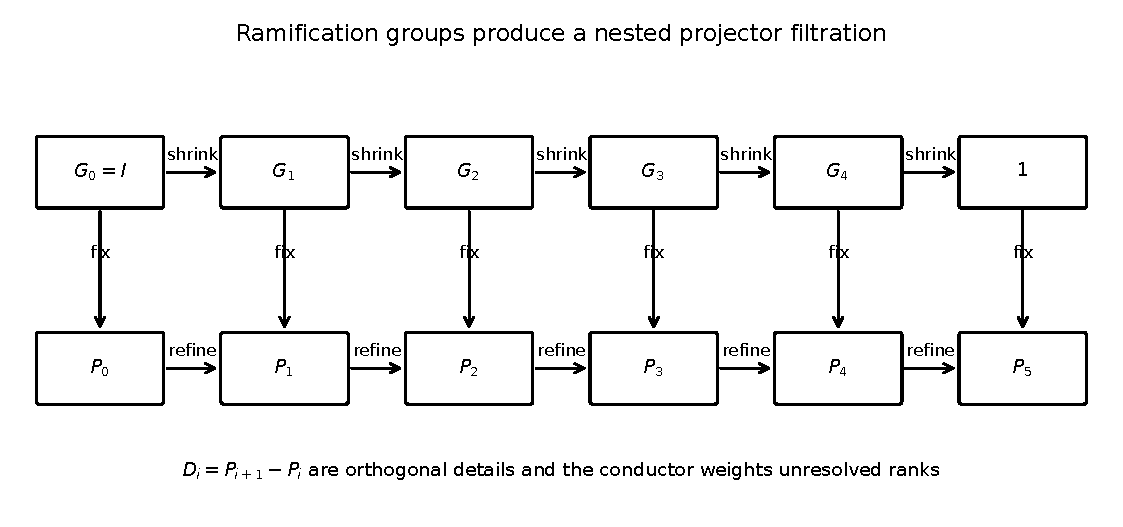
\includegraphics[width=.94\textwidth]{27_ramification_resolution.pdf}
\caption{The ramification groups give a nested projector filtration. Orthogonal detail packets carry the successive unresolved wild and tame structure.}
\label{fig:ramification_resolution}
\end{figure}

\section{Profinite, cohomological, and Tannakian descent}\label{sec:profinite_descent}

\subsection{Haar projectors and profinite limits}

\begin{theorem}[Haar fixed point projector]\label{thm:haar_projector}
Let \(G\) be a compact group and let \(U:G\to\mathcal U(\Hh)\) be a strongly continuous unitary representation. For every closed subgroup \(H\leq G\), define
\[
 \boxed{
 P_H
 =
 \int_HU_h\,d\mu_H(h),
 }
\]
where \(\mu_H\) is normalized Haar measure. Then \(P_H\) is the orthogonal projector onto \(\Hh^H\). If \(H\leq J\), then
\[
 P_HP_J=P_JP_H=P_J.
\]
If \(H\triangleleft G\), the fixed range carries the quotient action of \(G/H\).
\end{theorem}

\begin{proof}
Haar invariance gives self adjointness and idempotence exactly as finite averaging does. The range calculation follows from left invariance of Haar measure. The nesting and quotient conclusions are the same as in \cref{thm:reynolds_projector,thm:normality_centrality}.
\end{proof}

\begin{theorem}[Shrinking subgroup reconstruction]\label{thm:shrinking_subgroup_reconstruction}
Let \(G\) be profinite and let
\[
 H_1\supseteq H_2\supseteq\cdots
\]
be a neighborhood basis of the identity consisting of open normal subgroups. For every strongly continuous unitary representation,
\[
 \boxed{
 P_{H_n}\longrightarrow I
 }
\]
strongly. More generally, if \(N\triangleleft G\) is closed and \(H_n/N\) is a neighborhood basis of the identity in \(G/N\), then \(P_{H_n}\to P_N\) strongly.
\end{theorem}

\begin{proof}
For \(v\in\Hh\), strong continuity gives
\[
 \sup_{h\in H_n}\norm{U_hv-v}\longrightarrow0.
\]
Therefore
\[
 \norm{P_{H_n}v-v}
 \leq
 \int_{H_n}\norm{U_hv-v}\,d\mu_{H_n}(h)
 \longrightarrow0.
\]
The normal subgroup case follows by applying the identity result to the quotient representation on the \(N\) fixed subspace.
\end{proof}

\begin{corollary}[Finite quotient factorization]\label{cor:finite_quotient_factorization}
Every continuous finite dimensional complex representation of a profinite group has finite image and therefore factors through a finite quotient. The associated projector resolution is already visible at one finite Galois level.
\end{corollary}

\begin{proof}
The image is compact and totally disconnected. A compact subgroup of \(\GL_n(\CC)\) is a Lie group after conjugation into a unitary group. A totally disconnected compact Lie group is finite.
\end{proof}

\begin{corollary}[Absolute Galois resolution net]\label{cor:absolute_galois_resolution}
Let \(G_K\) be an absolute Galois group. Open normal subgroups, finite Galois extensions, and quotient symmetry packets form one directed profinite resolution system. In every continuous unitary realization, shrinking finite level projectors reconstruct the full representation strongly.
\end{corollary}

\begin{proof}
Open normal subgroups of \(G_K\) correspond to finite Galois extensions \Rcite{R29,R30}. Apply \cref{thm:shrinking_subgroup_reconstruction}.
\end{proof}

\begin{figure}[t]
\centering
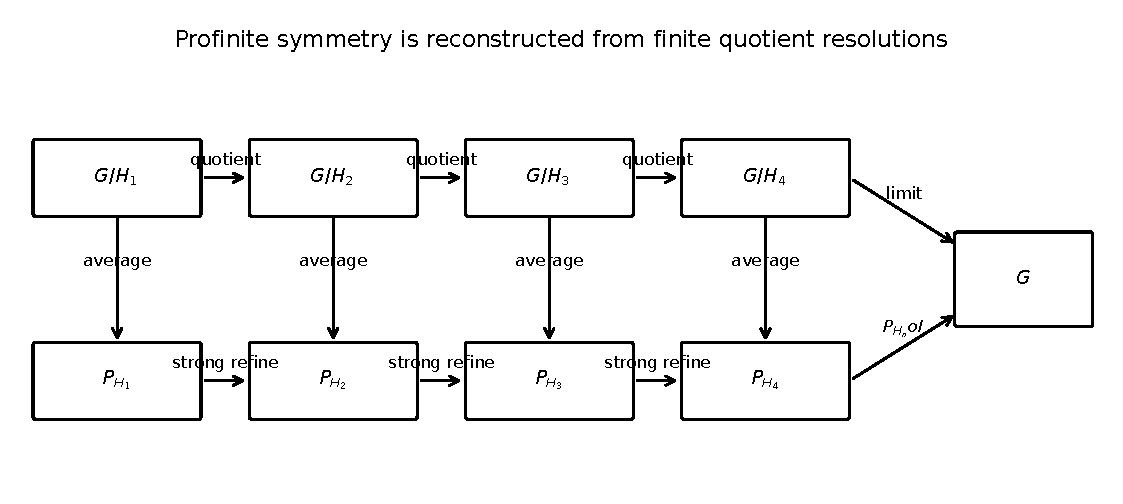
\includegraphics[width=.93\textwidth]{28_profinite_resolution.pdf}
\caption{Finite Galois quotients form an inverse system of symmetry charts, while the corresponding fixed projectors form a directed strong resolution.}
\label{fig:profinite_resolution}
\end{figure}

\subsection{Hilbert 90 as effective atlas descent}

\begin{definition}[Semilinear Galois cocycle]\label{def:semilinear_galois_cocycle}
Let \(L/K\) be finite Galois with group \(G\). A semilinear packet cocycle of rank \(n\) is a family
\[
 a_\sigma\in\GL_n(L)
\]
satisfying
\[
 \boxed{
 a_{\sigma\tau}
 =
 a_\sigma\,\sigma(a_\tau).
 }
\]
It defines the twisted semilinear action
\[
 \sigma\star v
 =
 a_\sigma\sigma(v)
\]
on \(L^n\).
\end{definition}

\begin{theorem}[Effective vector descent by Hilbert 90]\label{thm:hilbert90_resolution}
For every semilinear packet cocycle, there is \(B\in\GL_n(L)\) such that
\[
 \boxed{
 a_\sigma
 =
 B^{-1}\sigma(B)
 }
\]
for all \(\sigma\in G\). The fixed packet
\[
 W=(L^n)^{G,\star}
\]
is an \(n\) dimensional \(K\) vector space, and the natural map
\[
 \boxed{
 W\otimes_KL
 \longrightarrow
 L^n
 }
\]
is an isomorphism. Thus every linear semilinear atlas descends to one global vector packet.
\end{theorem}

\begin{proof}
The cocycle trivialization is nonabelian Hilbert 90 \Rcite{R24}. Conjugating the twisted action by \(B\) turns it into the ordinary coordinatewise Galois action. The fixed vectors then identify with \(K^n\), and scalar extension reconstructs \(L^n\).
\end{proof}

\begin{corollary}[Line descent]\label{cor:line_hilbert90}
For \(n=1\), every multiplicative cocycle is a coboundary:
\[
 H^1(G,L^\times)=1.
\]
Hence a line packet with compatible Galois transition scalars always has a global origin.
\end{corollary}

\begin{proof}
Apply \cref{thm:hilbert90_resolution} in rank one.
\end{proof}

\subsection{Projective descent and the Brauer obstruction}

\begin{theorem}[Brauer obstruction to projective packet descent]\label{thm:brauer_obstruction}
Projective semilinear descent data of rank \(n\) define a class in
\[
 H^1(G,\PGL_n(L)).
\]
The connecting map associated with
\[
 1\longrightarrow L^\times
 \longrightarrow\GL_n(L)
 \longrightarrow\PGL_n(L)
 \longrightarrow1
\]
sends that class to
\[
 \boxed{
 \delta(\alpha)
 \in
 H^2(G,L^\times)
 =
 \Br(L/K).
 }
\]
The class vanishes exactly when the projective atlas lifts to linear semilinear descent data. Nonzero classes classify central simple \(K\) algebras of degree \(n\) split by \(L\) \Rcite{R24,R27}.
\end{theorem}

\begin{proof}
This is the standard nonabelian cohomology exact sequence and the Galois cohomological description of the relative Brauer group. Vanishing means that the projective cocycle lifts to a \(\GL_n(L)\) cocycle. Hilbert 90 then makes the lifted atlas effective.
\end{proof}

\begin{corollary}[Resolution interpretation of the Brauer class]\label{cor:brauer_resolution_interpretation}
A projective packet atlas may satisfy every overlap law visible in \(\PGL_n\) while still failing to possess one global vector space realization. The Brauer class is the precise obstruction. When it vanishes, \cref{thm:hilbert90_resolution} supplies the global packet. When it does not, the descended object is a module over a central simple algebra rather than an ordinary vector space.
\end{corollary}

\begin{proof}
This is the two cases of \cref{thm:brauer_obstruction} interpreted through the recognition and gluing language of Resolution Theory.
\end{proof}

\begin{figure}[t]
\centering
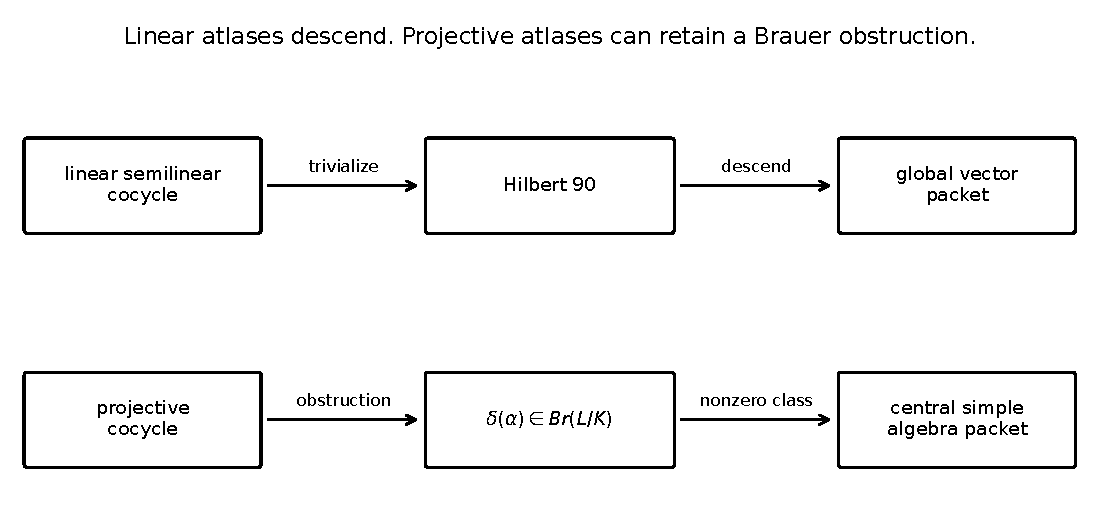
\includegraphics[width=.93\textwidth]{29_hilbert90_brauer.pdf}
\caption{Linear semilinear cocycles are removed by Hilbert 90. Projective cocycles can retain a degree two Brauer obstruction.}
\label{fig:hilbert90_brauer}
\end{figure}

\subsection{Etale Galois categories as permutation resolutions}

\begin{theorem}[Finite Galois category realization]\label{thm:galois_category_resolution}
Let \(X\) be a connected scheme with geometric point \(\bar x\). The fiber functor from finite etale covers of \(X\) to finite sets identifies that category with finite continuous \(\pi_1^{\mathrm{et}}(X,\bar x)\) sets \Rcite{R25}. For a finite fiber \(S\), the Hilbert space \(\ell^2(S)\) carries:
\begin{enumerate}
\item coordinate packet projectors indexed by points of \(S\)
\item orbit projectors indexed by transitive components
\item permutation transfer operators induced by covering morphisms
\item refinement maps induced by pullback of covers.
\end{enumerate}
Therefore finite etale Galois theory has a canonical permutation resolution realization, and the profinite fundamental group is the symmetry object of the fiber functor.
\end{theorem}

\begin{proof}
The categorical equivalence is the fundamental theorem of Galois categories. A finite set has its coordinate resolution in \(\ell^2(S)\). A continuous group action permutes those packets unitarily. Maps of finite covers induce equivariant maps of fibers, hence bounded packet transfers. Pullback refines the finite fiber product and its coordinate resolution.
\end{proof}

\subsection{Tannakian reconstruction and the monoidal boundary}

\begin{theorem}[Tannakian Galois reconstruction]\label{thm:tannakian_resolution}
Let \(\Ccal\) be a neutral Tannakian category over a field \(k\), and let
\[
 \omega:\Ccal\longrightarrow\operatorname{Vect}_k
\]
be a faithful exact tensor fiber functor. Then
\[
 \boxed{
 \mathcal G
 =
 \Aut^\otimes(\omega)
 }
\]
is an affine group scheme, and
\[
 \boxed{
 \Ccal\simeq\operatorname{Rep}_k(\mathcal G)
 }
\]
as tensor categories \Rcite{R26}. If \(\Ccal\) carries declared packet idempotents and refinement maps preserved by \(\omega\), they become concrete tensor compatible projector resolutions in every fiber.
\end{theorem}

\begin{proof}
The reconstruction statement is the neutral Tannakian theorem. Preservation of declared idempotents and refinements follows functorially from additivity and exact tensor compatibility.
\end{proof}

\begin{corollary}[The monoidal Galois boundary of Resolution Theory]\label{cor:monoidal_galois_boundary}
The monoidal enhancement problem in \cref{prop:monoidal_boundary} is exactly the point at which a Galois type symmetry object can be reconstructed. Ordinary faithful corner representation gives concrete packets and transfers. A faithful exact strong monoidal fiber functor additionally reconstructs the tensor automorphism group scheme.
\end{corollary}

\begin{proof}
Combine \cref{prop:monoidal_boundary,thm:tannakian_resolution}.
\end{proof}

\begin{figure}[t]
\centering
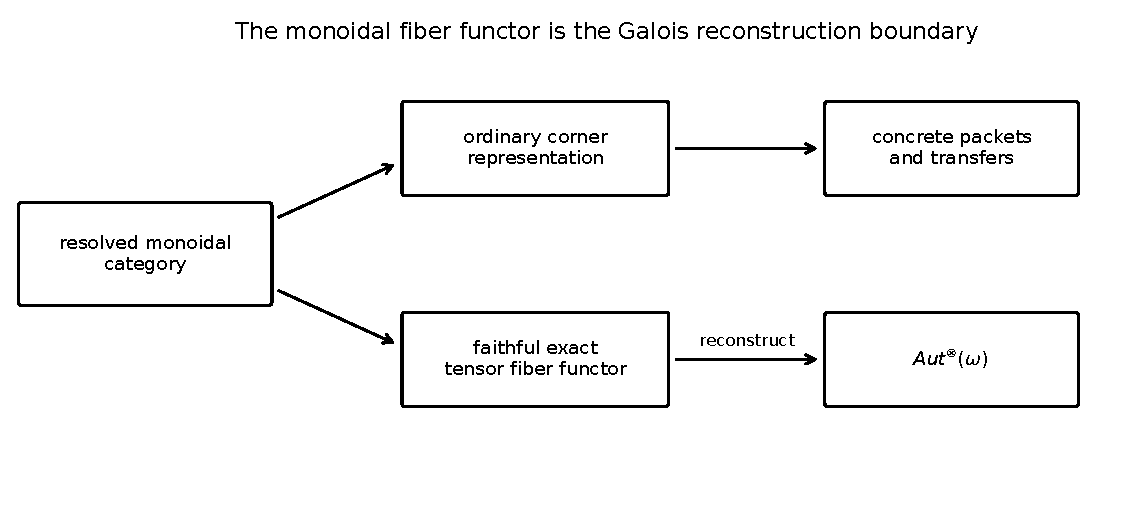
\includegraphics[width=.95\textwidth]{30_tannakian_boundary.pdf}
\caption{Ordinary corner representation realizes packets and transfers. A monoidal fiber functor crosses the Tannakian boundary and reconstructs a symmetry group scheme.}
\label{fig:tannakian_boundary}
\end{figure}

\begin{theorem}[Resolution Galois synthesis]\label{thm:resolution_galois_synthesis}
Under the declared semisimple hypotheses, finite Galois theory is a distinguished realization of Resolution Theory with the following correspondences:
\begin{enumerate}
\item subgroups correspond to fixed point projectors
\item intermediate fields correspond to fixed packet ranges
\item subgroup inclusion becomes reverse resolution order
\item normality becomes central compatibility and quotient compression
\item trace and norm become linear and nonlinear packet transfers
\item nonnormal extensions become conjugate projector atlases
\item double cosets become transition packets for induction and restriction
\item ramification groups become a nested resolution whose weighted unresolved ranks equal the Artin conductor
\item profinite Galois groups become inverse systems of finite quotient resolutions
\item Hilbert 90 gives effective linear atlas descent
\item Brauer classes measure projective descent failure
\item etale and Tannakian fiber functors reconstruct profinite and affine symmetry objects.
\end{enumerate}
\end{theorem}

\begin{proof}
The finite fixed point statements are \cref{thm:resolution_galois_correspondence,thm:normality_centrality,prop:galois_trace_norm,thm:galois_closure_atlas,thm:mackey_packet_decomposition}. Ramification is \cref{thm:ramification_details,thm:artin_conductor_resolution}. Profinite completion is \cref{thm:haar_projector,thm:shrinking_subgroup_reconstruction}. Cohomological descent is \cref{thm:hilbert90_resolution,thm:brauer_obstruction}. The categorical reconstruction statements are \cref{thm:galois_category_resolution,thm:tannakian_resolution}.
\end{proof}

\section{The closure theorem for Resolution Theory}\label{sec:closure}

The individual parts now combine into one dependency chain. The statement below records exactly what has been closed and which hypotheses are required.

\begin{theorem}[Expanded Resolution Theory closure theorem]\label{thm:closure}
Let \(\Acal\) be a unital resolved linking system with a finite named packet hierarchy. Under the additional hypotheses stated in the corresponding sections, the following conclusions hold.
\begin{enumerate}
\item \textbf{Concrete realization.} Every named object and packet idempotent has a faithful projector corner realization, and every abstract transfer corner is represented exactly.
\item \textbf{Recognition and refinement.} Forgetting Hilbert coordinates recovers the abstract resolved system, and every finite refinement equation survives representation.
\item \textbf{Finite transfer calculus.} Mixed corners reconstruct transfers, compose by packet paths, satisfy adjoint and Hilbert Schmidt identities, and admit optimal block compression with named residuals.
\item \textbf{Resolution geometry.} Finite resolutions carry a permutation invariant metric. Mixed block fields and transfer energy distributions are Lipschitz stable. Smooth resolution paths have canonical unitary transport and covariant transfer derivatives.
\item \textbf{Approximate reduction.} The commutant Laplacian measures total leakage. A positive commutant gap converts sufficiently small leakage into a nearby exact reducing packet.
\item \textbf{Weighted inversion.} Admissibly weighted block Schur classes form Banach star algebras. Neumann inversion and block diagonal dominance give inverse packet path expansions and quantitative off diagonal decay.
\item \textbf{Countable categorical completion.} Bounded maps reconstruct strongly, compact and Schatten maps in their natural norms, linking elements through norm windows, and multipliers through strict windows. Packet idempotents split as Karoubi objects and normal states converge in trace norm.
\item \textbf{Unbounded and measurable completion.} Reducing packets control graph norms, forms, resolvents, bounded transforms, strong resolvent limits, unitary dynamics, and measurable chart covariance. Commutators bound dynamical leakage.
\item \textbf{Nonlinear completion.} Smooth maps have exact packet jets and operadic composition. Weighted analytic classes support local inversion and Newton certificates. Countable multilinear maps, semilinear Duhamel trees, Hamiltonian packets, and stochastic Itô corrections have resolved forms.
\item \textbf{Logic.} Finite Resolution Logic is sound and complete on finite atomic fibers. Countable atomic Boolean and complete lattice certificate fibers admit exact pullback and quantifier adjunctions with sound packet error transport.
\item \textbf{Realizations.} Fourier, wavelet, polyphase, quantum, and arithmetic systems satisfy the resolved axioms. In the arithmetic realization, the sieve line and survivor residual are orthogonal, and the additive to multiplicative Gauss transform is a change of resolution.
\item \textbf{Galois realization.} Finite subgroup fixed objects are orthogonal projector ranges. Normality is central compatibility, quotient actions are compressed symmetries, trace and norm are packet transfers, Galois closures are projector atlases, ramification is a nested detail filtration, profinite groups admit Haar projectors, and cohomological or Tannakian descent records the remaining global symmetry data.
\end{enumerate}
\end{theorem}

\begin{proof}
The representation, recognition, and refinement claims are \cref{thm:universal_projector_representation,thm:recognition,prop:refinement_naturality}. The finite transfer and compression statements are \cref{thm:mixed_blocks,thm:packet_parseval,thm:selective_compression,thm:budget_tolerance}. The geometric and gap statements are \cref{thm:resolution_metric,thm:block_field_stability,thm:kato_transport,thm:commutant_gap_stability}. Weighted inversion is \cref{thm:weighted_schur_algebra,thm:resolved_neumann_inverse,thm:block_inverse_paths}. Countable categorical completion follows from \cref{thm:strong_reconstruction,thm:compact_truncation,thm:countable_linking,thm:strict_windows,thm:karoubi_packet_splitting,thm:expanded_categorical_completion}. The unbounded and measurable statements are \cref{thm:unbounded_direct_sum,thm:graph_norm,thm:form_packet_reconstruction,thm:strong_resolvent_windows,prop:dynamical_leakage,thm:decomposable_reconstruction,prop:measurable_covariance}. The nonlinear statements are \cref{thm:multilinear_reconstruction,thm:faa_di_bruno,thm:analytic_composition,thm:near_identity_inverse,thm:countable_multilinear,thm:resolved_newton,thm:duhamel_pruning,prop:hamiltonian_packets,thm:ito_packet_generator}. The logic statements are \cref{thm:indexed_semantics,thm:countable_boolean_doctrine,thm:quantitative_fiber_adjoints,thm:countable_error_transport}. The realization statements are \cref{thm:fourier_realization,thm:wavelet_realization,prop:quantum_realization,thm:arithmetic_polyphase,thm:arithmetic_sieve_line,thm:gauss_resolution_change}. The Galois realization is \cref{thm:resolution_galois_synthesis}.
\end{proof}

\begin{corollary}[Commuting representation and refinement diagram]\label{cor:commuting_diagram}
Let \(e=\sum_\alpha e_\alpha\) be a declared finite refinement and let \(T\) be any transfer. Under every faithful realization \(\pi\), the diagram
\[
 \begin{array}{ccc}
 e\Acal e&\xrightarrow{\ T\ }&f\Acal f\\
 \downarrow\pi&&\downarrow\pi\\
 \pi(e)\pi(\Acal)\pi(e)&\xrightarrow{\ \pi(T)\ }&\pi(f)\pi(\Acal)\pi(f)
 \end{array}
\]
commutes, while
\[
 \pi(e)=\sum_\alpha\pi(e_\alpha)
\]
preserves the refinement equation. The same naturality holds for every finite chain of refinements.
\end{corollary}

\begin{proof}
Multiplicativity of \(\pi\) gives commutativity of the transfer square. Refinement naturality is \cref{prop:refinement_naturality}. Iteration gives the final assertion.
\end{proof}

\begin{corollary}[Fourier analysis as a resolved specialization]\label{cor:fourier_specialization}
Finite Fourier analysis is a specialization of Resolution Theory obtained by choosing the character projectors of a finite abelian group. Fourier reconstruction, Parseval, and convolution diagonalization are consequences of the general packet reconstruction, packet energy, and invariant transfer principles.
\end{corollary}

\begin{proof}
Apply \cref{thm:fourier_realization} inside \cref{thm:closure}.
\end{proof}

\begin{figure}[t]
\centering
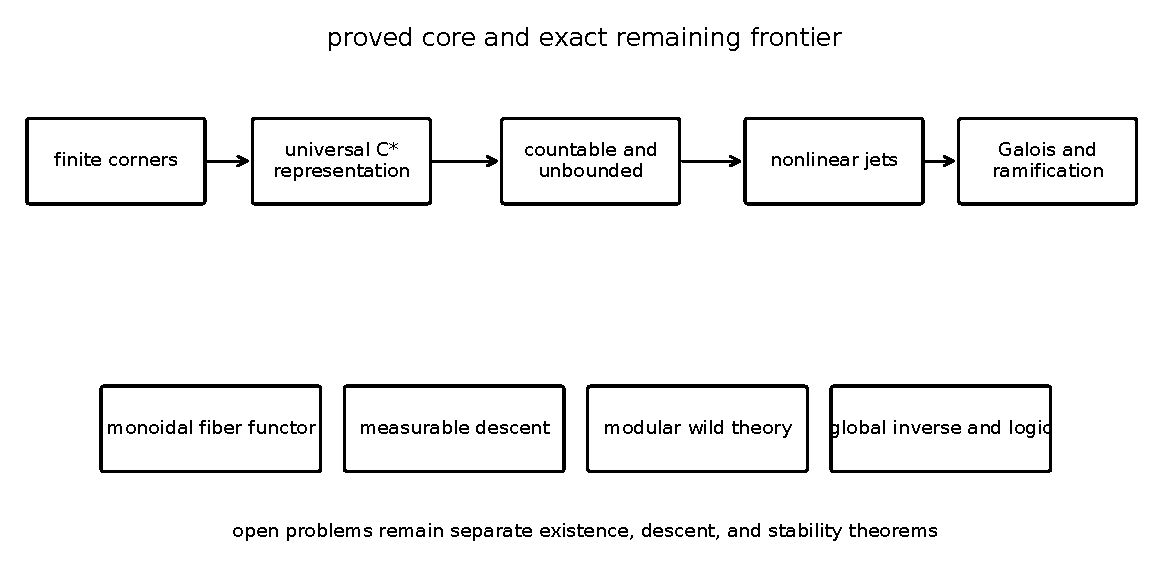
\includegraphics[width=.95\textwidth]{12_boundary_map.pdf}
\caption{The closed theorem chain and the boundaries that require additional hypotheses.}
\label{fig:boundary_map}
\end{figure}

\section{Exact boundaries and open problems}\label{sec:boundaries}

The expanded theory closes several boundaries left open in the earlier finite edition. It still does not imply that every representation is useful, computationally inexpensive, globally inverse closed, statistically stable, or compatible with every categorical enhancement.

\subsection{Monoidal realization}

\begin{problem}[Monoidal fiber problem]\label{prob:monoidal}
Characterize resolved monoidal \(C^*\) categories admitting a faithful unitary strong monoidal dagger functor into Hilbert spaces. Determine which packet refinements, weighted norms, and nonlinear tensor interactions are preserved by such a functor.
\end{problem}

Ordinary projector corner representability does not manufacture a monoidal fiber functor \Rcite{R12}.

\subsection{Measurable resolution and descent}

Direct integrals provide measurable packet reconstruction and unitary chart covariance. They do not by themselves supply descent for arbitrary local packet atlases.

\begin{problem}[Measurable resolution descent]\label{prob:measurable}
Develop a representation and descent theorem for measurable resolved fields with nontrivial overlap cocycles, measurable refinements, and higher compatibility data. Identify hypotheses under which local resolved models form a stack.
\end{problem}

\subsection{Modular and wild Galois resolution}

The semisimple projector embedding uses averaging by subgroup order. It does not survive unchanged when the coefficient characteristic divides that order.

\begin{problem}[Modular and wild Galois resolution]\label{prob:modular_galois}
Construct a derived or finite flat Resolution Theory for modular Galois actions in which fixed points need not be exact, Reynolds projectors may fail to exist, and wild ramification carries integral torsion. Relate the resulting packet complexes to group schemes, ramification filtrations, and deformation theory.
\end{problem}

\subsection{Hopf and quantum Galois resolution}

\begin{problem}[Hopf Galois resolution]\label{prob:hopf_galois}
Extend the subgroup projector, fixed algebra, quotient compression, and descent results from finite groups to Hopf algebra coactions, compact quantum groups, and Hopf Galois extensions. Determine which conditional expectations and monoidal fiber functors yield faithful resolved realizations.
\end{problem}

\subsection{Global weighted inverse closure}

The local resolved Wiener theorem is complete near the identity and under block diagonal dominance. Global spectral invariance remains separate.

\begin{problem}[Global resolved Wiener problem]\label{prob:wiener}
Find geometric and weight conditions under which every element of a weighted packet transfer algebra that is invertible in the ambient operator algebra has its inverse in the same weighted algebra. Determine sharp inverse decay without a small norm hypothesis.
\end{problem}

\subsection{Learning and perturbation stability}

The metric and commutant gap theorems control a declared projector family. Learned projectors require statistical analysis of how that family is obtained.

\begin{problem}[Learned resolution stability]\label{prob:learning}
Prove perturbation, generalization, and leakage bounds for projectors learned from finite data. Separate approximation error, estimation error, gap collapse, packet matching ambiguity, and downstream transfer error.
\end{problem}

\subsection{Measurable Resolution Logic}

Countable atomic predicate and certificate fibers are complete. General measurable predicates require additional semantics.

\begin{problem}[Measurable Resolution Logic]\label{prob:infinite_logic}
Construct an indexed semantics for measurable resolutions, almost everywhere predicates, conditional expectations, and analytic certificates. Prove soundness and an appropriate completeness theorem under declared measurability and integrability hypotheses.
\end{problem}

\subsection{Algorithmic resolution discovery}

\begin{problem}[Resolution discovery]\label{prob:discovery}
Given an operator family, a cost model, and an error tolerance, determine complexity bounds for finding a resolution that minimizes transfer density, leakage, inverse decay, or execution cost. Establish hardness results and approximation guarantees.
\end{problem}

\subsection{Arithmetic analytic estimates}

The arithmetic realization gives exact packet, sieve, and character identities. Analytic estimates remain number theoretic input rather than formal consequences of the universal calculus.

\begin{problem}[Arithmetic band estimates]\label{prob:arithmetic_estimates}
Obtain sharp individual and averaged estimates for the survivor character bands arising from prime packet refinement. Determine when the resolved coordinates yield stronger localization of exceptional arithmetic behavior than existing variance methods.
\end{problem}

\begin{remark}[No universal optimal chart]\label{rem:no_universal_chart}
Different tasks can prefer incompatible resolutions. Noncommuting projector families may have no exact common refinement. Resolution Theory therefore supports atlases, covariant transport, and task dependent planners rather than one universal basis.
\end{remark}

\section{Conclusion}\label{sec:conclusion}

Resolution Theory begins with the exact corner identity
\[
 T=\sum_{a,i}Q_aTP_i
\]
and keeps the projectors, packet blocks, refinement maps, residuals, and certificates inside the mathematical object. The expanded theory now adds a geometry of resolution space, quantitative stability of block fields, canonical transport of moving packet systems, and a commutant gap theorem turning small leakage into nearby exact structure.

Weighted packet algebras make inverse structure visible as path summation. Countable completion distinguishes norm, strict, strong, trace norm, graph norm, and measurable reconstruction. Nonlinear resolution treats derivatives as typed hyperedges and extends to Newton certificates, semilinear dynamics, Hamiltonian structure, and stochastic quadratic variation. Countable atomic Resolution Logic carries truth and quantitative evidence through infinite packet refinements.

Fourier, wavelet, polyphase, quantum, arithmetic, and Galois systems are not parallel analogies. They are concrete charts of the same resolved architecture. The arithmetic chart shows how deterministic sieve geometry and multiplicative character energy arise from successive changes of resolution. The Galois chart shows how symmetries, fixed objects, quotient actions, ramification, and descent become projector ranges, conditional expectations, nested detail packets, cocycles, and fiber functors.

The theory does not promise that every problem has a useful decomposition or that a universal representation is computationally optimal. It also does not replace modular Galois theory, etale homotopy, or Tannakian reconstruction by formal projector notation. Its contribution is to make representation choice, motion, approximation, inversion, information loss, fixed structure, and descent obstruction explicit, to prove which structures survive transport and refinement, and to isolate the exact hypotheses still required for monoidal, measurable, modular, global inverse, statistical, and arithmetic completion.

\end{document}